\documentclass[12pt,letterpaper]{article}
\newcommand\hmmax{0}
\newcommand\bmmax{0}
\usepackage[T1]{fontenc}
\usepackage{lmodern}
\usepackage[utf8]{inputenc}
\usepackage{geometry}
\usepackage{ragged2e}
\usepackage{nicefrac}
\usepackage{booktabs}
\usepackage{amsfonts}
\usepackage{dsfont}
\usepackage{cancel}
\usepackage{mathtools}
\usepackage{datetime}
\usepackage{bm}
\usepackage{paralist}
\usepackage{changepage}
\usepackage{amsthm}
\usepackage{verbatim}
\usepackage{amsmath,amssymb}
\usepackage{graphicx}
\usepackage{emptypage}
\usepackage{mathabx}
\usepackage{newlfont}
\usepackage{tikz-cd}
\usepackage{tikz}
\usepackage[all,cmtip]{xy}
\usepackage[bottom]{footmisc}
\usepackage[titletoc,title]{appendix}
\usepackage{chngcntr}
\usepackage{apptools}
\usepackage{listings}
\usepackage{color}
\usepackage{sgame, tikz}
\let\widering\relax
\usepackage{kpfonts}
\usepackage{natbib}
\AtAppendix{\counterwithin{lem}{section}}
\usepackage{caption}
\usepackage{subcaption}
\usepackage{float}
\usepackage{thmtools,thm-restate}
\usepackage{epigraph}
\usepackage{xr-hyper}
\usepackage[colorlinks=true,allcolors=blue]{hyperref}
\usepackage{ctex}

\graphicspath{{f:/3.笔记、导图与Pre/1.论文阅读与笔记/ambiguity/Yang_Stochastic_Optimization_Coupling/}}

\newenvironment{original}{\color{black}}{}
\newenvironment{translation}{\color{blue}}{}

\newcommand\bref[1]{{\hypersetup{linkcolor=blue}\autoref{#1}}}
\makeatletter
\renewcommand\@makefnmark{\hbox{\@textsuperscript{\normalfont\color{black}\@thefnmark}}}
\makeatother
\DeclareMathOperator*{\argmax}{\arg\!\max}
\DeclareMathOperator*{\argmin}{\arg\!\min}
\newcommand*\supp{\mathrm{supp}}
\usepackage{wasysym}
\hypersetup{colorlinks,linkcolor=blue,allcolors=blue}
\usepackage{sgamevar}
\hypersetup{urlcolor=blue}
\newcommand{\numberset}{\mathbb}
\newcommand\myfunc[5]{
  \begingroup
  \setlength\arraycolsep{0pt}
  #1\colon\begin{array}[t]{c >{{}}c<{{}} c}
             #2 & \longrightarrow & #3 \\ #4 & \longmapsto & #5
          \end{array}
  \endgroup}
\theoremstyle{plain}
\newtheorem{cor}{Corollary}
\newtheorem{prop}{Proposition}
\newtheorem{claim}{Claim}
\newtheorem{theorem}{Theorem}
\newtheorem{lemma}{Lemma}
\theoremstyle{definition}
\newtheorem{ex}{Example}
\newtheorem{observation}{Observation}
\newtheorem{fact}{Fact}
\newtheorem{property}{Property}
\newtheorem{thm}{Theorem}
\newtheorem{asm}{Assumption}
\newtheorem{asmB}{Assumption}
\renewcommand\theasm{A\arabic{asm}}
\renewcommand\theasmB{B\arabic{asmB}}
\newtheorem{manualasminner}{Assumption}
\newenvironment{manualasm}[1]{
  \renewcommand\themanualasminner{#1}
  \manualasminner
}{\endmanualasminner}
\newtheorem{defn}{Definition}
\newtheorem{lem}{Lemma}
\newtheorem{taggedlemmax}{Lemma}

\newenvironment{taggedlemma}[1]
 {\renewcommand\thetaggedlemmax{#1}\taggedlemmax}
 {\endtaggedlemmax}
 \newtheorem{taggedpropositionx}{Proposition}
\newenvironment{taggedproposition}[1]
{\renewcommand\thetaggedpropositionx{#1}\taggedpropositionx}
 {\endtaggedpropositionx}
 \newtheorem{taggedtheoremx}{Theorem}
\newenvironment{taggedtheorem}[1]
{\renewcommand\thetaggedtheoremx{#1}\taggedtheoremx}
 {\endtaggedtheoremx}
\newtheorem{taggedcorollaryx}{Corollary}
 \newenvironment{taggedcorollary}[1]
{\renewcommand\thetaggedcorollaryx{#1}\taggedcorollaryx}
 {\endtaggedcorollaryx}
\allowdisplaybreaks
\makeatletter
\renewenvironment{proof}[1][\proofname]{
  \par\pushQED{\qed}\normalfont
  \topsep6\p@\@plus6\p@\relax
  \trivlist\item[\hskip\labelsep\bfseries#1\@addpunct{.}]
  \ignorespaces
}{
  \popQED\endtrivlist\@endpefalse
}
\makeatother
\theoremstyle{remark}
\newtheorem{rmk}{Remark}
\newtheorem{alg}{Algorithm}
\newtheorem*{nota}{Notation}
\let\emptyset\varnothing
\DeclareMathOperator{\lcm}{lcm}
\DeclareMathOperator{\E}{\mathds{E}}
\renewcommand{\P}{\mathds{P}}
\newcommand{\Pc}{\mathcal{P}}
\newcommand{\F}{\mathcal{F}}
\newcommand{\C}{\mathcal{C}}
\newcommand{\B}{\mathcal{B}}
\newcommand{\R}{\mathds{R}}
\newcommand{\Q}{\mathds{Q}}
\newcommand{\cQ}{\mathcal{Q}}
\newcommand{\N}{\mathds{N}}
\newcommand{\Z}{\mathds{Z}}
\renewcommand{\H}{\mathcal{H}}
\newcommand{\A}{\mathcal{A}}
\renewcommand{\S}{\mathcal{S}}
\newcommand{\M}{\mathcal{M}}
\newcommand{\K}{\mathcal{K}}
\newcommand{\Y}{\mathcal{Y}}
\newcommand{\IC}{\text{IC}}
\newcommand{\IR}{\text{IR}}
\newcommand{\MR}{\text{MR}}
\newcommand{\V}{\text{Var}}
\newcommand{\Cov}{\text{Cov}}
\newcommand{\Rev}{\text{Rev}}
\newcommand{\Exp}{\mathrm{exp}}
\newcommand{\lb}{\underline}
\newcommand{\ub}{\overline}
\DeclareMathOperator{\sign}{sign}
\newcommand{\ind}{\mathds{1}}
\newcommand\eqas{\stackrel{a.s.}{=}}
\newcommand\eqid{\stackrel{d}{=}}
\newcommand\as{\xrightarrow{a.s.}}
\newcommand{\tv}{\xrightarrow{t.v.}}
\newcommand{\wk}{\xRightarrow{w}}
\newcommand\id{\xrightarrow{D}}
\newcommand\ip{\xrightarrow{p}}
\newcommand{\Ext}{\mathrm{ext}}
\newcommand{\io}{\text{ i.o. }}
\newcommand{\ev}{\text{  ev. }}
\renewcommand{\r}{\rightarrow}
\renewcommand{\l}{\leftarrow}
\newcommand{\lr}{\leftrightarrow}
\renewcommand{\epsilon}{\varepsilon}
\renewcommand*\d{\mathop{}\!\mathrm{d}}
\newcommand*\circled[1]{\tikz[baseline=(char.base)]{
            \node[shape=circle,draw,inner sep=2pt] (char) {#1};}}
\newcommand{\join}{\vee}
\newcommand{\meet}{\wedge}
\newcommand{\X}{\mathcal{X}}
\newcommand{\vsmall}{\vskip 5}
\newcommand{\vmedium}{\vskip 10}
\newcommand{\vbig}{\vskip 20}
\DeclareMathOperator*{\cart}{\bigtimes}
\setlength{\epigraphrule}{0pt}
\usepackage{setspace}
\def\blank{\medskip\hrule\medskip}
\newcommand\defeq{\mathrel{\overset{\makebox[0pt]{\mbox{\normalfont\scriptsize\sffamily def}}}{=}}}
\linespread{1.25}
\geometry{left=1.0in,right=1.0in,top=1.0in,bottom=1.0in, heightrounded}
\theoremstyle{definition}
\newtheorem{definition}{Definition}
\reversemarginpar


\newdate{draftdate}{02}{10}{2023}
\usdate

\usepackage[nameinlink]{cleveref}
\crefname{manualasm}{assumption}{assumptions}
\crefname{taggedtheoremx}{theorem}{theorems}
\crefname{taggedcorollaryx}{corollary}{corollaries}
\crefname{cor}{corollary}{corollaries}
\crefalias{prop}{proposition}
\crefname{claim}{claim}{claims}
\crefname{ex}{example}{examples}
\crefname{defn}{definition}{definitions}
\crefname{rmk}{remark}{remarks}
\crefname{alg}{algorithm}{algorithms}
\crefname{lem}{lemma}{lemma}
\usepackage{xparse}
\makeatletter
\newlength{\eqtaghshift}
\setlength{\eqtaghshift}{-1.5em}
\newlength{\eqtagvshift}
\setlength{\eqtagvshift}{0.65\baselineskip}
\NewDocumentCommand{\eqtag}{ O{\eqtaghshift} O{\eqtagvshift} m m }{
  \hypertarget{#4}{}
  \vadjust{
    \nobreak
    \smash{
      \raisebox{#2}{
        \hbox to 0pt{
          \hspace*{#1}
          \hbox to \textwidth{\hfill \textnormal{(#3)}}
          \hss
        }
      }
    }
  }
}

\makeatother

\DeclareRobustCommand{\weqref}[2]{
  \leavevmode\nobreak\hbox{\hyperlink{#2}{\textup{(#1)}}}
}



\begin{document}
\title{\textbf{Stochastic Optimization and Coupling}\thanks{We thank Ryota Iijima, Ravi Jagadeesan, Jesse Shapiro, Ludvig Sinander, Andrzej Skrzypacz, and Tomasz Strzalecki for helpful comments and suggestions.}
}
\author{Frank Yang\thanks{Department of Economics, Harvard University. Email: fyang@fas.harvard.edu.} \and Kai Hao Yang\thanks{School of Management, Yale University. Email: kaihao.yang@yale.edu.}}
\date{\today
}
\maketitle

\begin{original}
\begin{abstract}
We study optimization problems in which a linear functional is maximized over probability measures that are dominated by a given measure according to an integral stochastic order in an arbitrary dimension. We show that the following four properties are equivalent for any such order: (i) the test function cone is closed under pointwise minimum, (ii) the value function is affine, (iii) the solution correspondence has a convex graph with decomposable extreme points, and (iv) every ordered pair of measures admits an order-preserving coupling. As corollaries, we derive the extreme and exposed point properties involving integral stochastic orders such as multidimensional mean-preserving spreads and stochastic dominance. Applying these results, we generalize Blackwell's theorem by completely characterizing the comparisons of experiments that admit two equivalent descriptions---through instrumental values and through information technologies. We also show that these results immediately yield new insights into information design, mechanism design, and decision theory.
\\


\noindent\textbf{Keywords:} Stochastic orders, extreme points, Blackwell order, Strassen's theorem, comparisons of experiments, Bayes' rule, information design, mechanism design.


\end{abstract}
\end{original}
\begin{translation}
\begin{abstract}
我们研究一类优化问题，其中线性泛函在概率测度上被最大化，这些测度在任意维度上按照积分随机序被给定测度所支配。我们证明了对任何此类序，以下四个性质是等价的：(i) 检验函数锥在逐点最小值下封闭，(ii) 值函数是仿射的，(iii) 解对应具有凸图且极端点可分解，以及(iv) 每一对有序测度都存在保序耦合。作为推论，我们推导了涉及积分随机序（如多维均值保留展形和随机占优）的极端点和暴露点性质。应用这些结果，我们推广了Blackwell定理，完全刻画了那些允许两种等价描述——通过工具价值和通过信息技术——的实验比较。我们还表明，这些结果立即为信息设计、机制设计和决策理论提供了新的洞见。
\\


\noindent\textbf{关键词：} 随机序，极端点，Blackwell序，Strassen定理，实验比较，贝叶斯法则，信息设计，机制设计。

\end{abstract}
\end{translation}

\setcounter{page}{1}
\newpage

\addtocontents{toc}{\protect\setcounter{tocdepth}{2}}
\newpage

\section{Introduction}

\begin{original}
Many economic problems involve comparing or choosing probability measures. A celebrated example is the Blackwell order, which compares the distributions of posterior beliefs to understand which posterior distributions result from a more informative experiment that uniformly improves the payoff of a decision maker for all decision problems. The Blackwell order is an example of \textit{\textbf{integral stochastic orders}} where the comparisons are defined with respect to a set of test functions, which in Blackwell's case is the set of convex functions representing the indirect utility functions from decision problems.
\end{original}
\begin{translation}
许多经济问题涉及概率测度的比较或选择。一个著名的例子是Blackwell序，它比较后验信念的分布，以理解哪些后验分布源于一个在所有决策问题中都能一致提高决策者收益的更具信息量的实验。Blackwell序是\textit{\textbf{积分随机序}}的一个例子，其中比较是相对于一组检验函数定义的，在Blackwell的情形中，这组检验函数是代表决策问题的间接效用函数的凸函数集。
\end{translation}

\begin{original}
We study abstract optimization problems involving probability measures that are dominated by a given measure according to an integral stochastic order. Formally, we aim to understand the properties of
\[\max_{\nu \preceq_\C \mu} \int f(x) \nu(\d x)\,,\]
where $\mu$ is a given measure on some abstract set $X$, $\C$ is a cone of test functions that defines an integral stochastic order, and $\nu$ is the endogenous measure being chosen. We obtain new structural properties of this optimization problem. As corollaries, we derive the extreme and exposed point properties involving integral stochastic orders such as multidimensional mean-preserving spreads and stochastic dominance. Applying these results, we generalize Blackwell's theorem by completely characterizing the comparisons of experiments that admit two equivalent descriptions---through instrumental values and through information technologies. We also show that these results immediately yield new insights into information design, mechanism design, and decision theory.
\end{original}
\begin{translation}
我们研究抽象的优化问题，其中概率测度按照积分随机序被给定测度所支配。形式上，我们旨在理解以下问题的性质：
\[\max_{\nu \preceq_\C \mu} \int f(x) \nu(\d x)\,,\]
其中$\mu$是某个抽象集合$X$上的给定测度，$\C$是定义积分随机序的检验函数锥，$\nu$是被选择的内生测度。我们获得了该优化问题的新的结构性质。作为推论，我们推导了涉及积分随机序（如多维均值保留展形和随机占优）的极端点和暴露点性质。应用这些结果，我们推广了Blackwell定理，完全刻画了那些允许两种等价描述——通过工具价值和通过信息技术——的实验比较。我们还表明，这些结果立即为信息设计、机制设计和决策理论提供了新的洞见。
\end{translation}

\paragraph{Abstract Results.}\hspace{-2mm}

\begin{original}
Before discussing the economic applications, we start by describing our abstract results. Let $V^\star_f(\mu)$ denote the \textit{\textbf{value function}} of the optimization problem and $X^\star_f(\mu)$ denote its \textit{\textbf{solution correspondence}}. It is easy to see that $V^\star_f(\mu)$ is a concave functional and $X^\star_f(\mu)$ is convex-valued, but in general both objects can be very complex. Our results pertain to necessary and sufficient conditions on the stochastic order under which the optimization problem drastically simplifies and the stochastic comparison itself yields a tractable structure.
\end{original}
\begin{translation}
在讨论经济应用之前，我们首先描述我们的抽象结果。令$V^\star_f(\mu)$表示优化问题的\textit{\textbf{值函数}}，$X^\star_f(\mu)$表示其\textit{\textbf{解对应}}。容易看出$V^\star_f(\mu)$是一个凹泛函，$X^\star_f(\mu)$是凸值的，但一般而言这两个对象都可能非常复杂。我们的结果涉及随机序的充分必要条件，在这些条件下优化问题大幅简化，且随机比较本身产生了可处理的结构。
\end{translation}

\begin{original}
We say that the cone of test functions $\C$ is \textit{\textbf{min-closed}} if it is closed under pointwise minimum, i.e., $\min\{g_1, g_2\} \in \C$ for $g_1, g_2 \in \C$. We say that the stochastic order $\preceq_\C$ admits \textit{\textbf{order-preserving couplings}} if for any $\nu \preceq_\C \mu$ there exists a Markov kernel $P$ such that $\nu = P * \mu$ and $P * \delta_x \preceq_\C \delta_x$ for all $x$, i.e., there exists a Strassen-type coupling.\footnote{As we explicitly define later, we use the notation $P*\mu$ to denote the measure obtained by applying the transition kernel $P$ to $\mu$. That is, $P*\mu(\d y):=\int P(\d y \mid x)\mu(\d x)$.}
\end{original}
\begin{translation}
我们称检验函数锥$\C$是\textit{\textbf{最小-封闭}}的，如果它在逐点最小值下封闭，即对任意$g_1, g_2 \in \C$有$\min\{g_1, g_2\} \in \C$。我们称随机序$\preceq_\C$存在\textit{\textbf{保序耦合}}，如果对任意$\nu \preceq_\C \mu$存在Markov核$P$使得$\nu = P * \mu$且对所有$x$有$P * \delta_x \preceq_\C \delta_x$，即存在Strassen型耦合。\footnote{如我们后文明确定义的，我们用记号$P*\mu$表示将转移核$P$应用于$\mu$所得到的测度，即$P*\mu(\d y):=\int P(\d y \mid x)\mu(\d x)$。}
\end{translation}

\begin{original}
Our key structural result is an equivalence theorem (\Cref{thm:main}) that establishes the following four-way equivalence:
\begin{itemize}
    \item[(a)] $\C$ is min-closed.
    \item[(b)] $V^\star_f(\mu)$ is affine for all $f$.
    \item[(c)] $\preceq_\C$ admits order-preserving couplings.
    \item[(d)] $X^\star_f(\mu)$ has a convex graph whose extreme points are ``decomposable'' for all $f$.
\end{itemize}
By ``decomposable'' extreme points, we mean that every extreme point $(\mu, \nu)$ of the graph of $X^\star_f$ is one where $\mu$ is an extreme point of its convex domain, and $\nu$ is an extreme point of $X^\star_f(\mu)$ given $\mu$---we refer to such a graph as a \textit{\textbf{trapezoid graph}}, as illustrated by \Cref{fig:trapezoid}.
\end{original}
\begin{translation}
我们的关键结构结果是一个等价定理（\Cref{thm:main}），建立了以下四向等价：
\begin{itemize}
    \item[(a)] $\C$是最小-封闭的。
    \item[(b)] 对所有$f$，$V^\star_f(\mu)$是仿射的。
    \item[(c)] $\preceq_\C$存在保序耦合。
    \item[(d)] 对所有$f$，$X^\star_f(\mu)$具有凸图且其极端点可分解。
\end{itemize}
所谓``可分解''极端点，是指$X^\star_f$的图的每个极端点$(\mu, \nu)$满足：$\mu$是其凸定义域的极端点，$\nu$是给定$\mu$下$X^\star_f(\mu)$的极端点——我们将这种图称为\textit{\textbf{梯形图}}，如\Cref{fig:trapezoid}所示。
\end{translation}

\begin{figure}
\centering
\tikzset{
solid node/.style={circle,draw,inner sep=1.25,fill=black},
hollow node/.style={circle,draw,inner sep=1.25}
}
\begin{tikzpicture}[scale=8]
\fill [blue!30!white] (0,0.2)--(0.5,0.1)--(0.5,0.4)--(0,0.3);
\draw [<->, ultra thick] (0,0.6) node (yaxis) [above] {\footnotesize$X^\star_f(\mu)$}
        |- (0.6,0) node (xaxis) [right] {\footnotesize$\mu$};
\draw [very thick] (0,0.2)--(0.5,0.1);
\draw [very thick] (0,0.3)--(0.5,0.4);
\draw (0,0) node [below=2pt] {\footnotesize $0$};
\draw (0.5,0) node [below=2pt] {\footnotesize $1$};
\draw (0,0.3) node [solid node] {};
\draw (0,0.2) node [solid node] {};
\draw (0.5,0.1) node [solid node] {};
\draw (0.5,0.4) node [solid node] {};
\draw [very thick] (0.5,0.1)--(0.5,0.4);
\end{tikzpicture}
\begin{original}
\caption{Trapezoid Graph. $X=\{0,1\}$.}
\end{original}
\begin{translation}
\caption{梯形图。$X=\{0,1\}$。}
\end{translation}
\medskip
    \small
    \justifying
    \noindent
\begin{original}
    The colored area represents the graph of a solution correspondence $X^\star_f$. The extreme points of this set are pairs $(\mu,\nu)$, where $\mu$ is an extreme point of $\Delta(X)$ and $\nu$ is an extreme point of $X^\star_f(\mu)$.
\end{original}
\begin{translation}
    着色区域表示解对应$X^\star_f$的图。该集合的极端点是成对$(\mu,\nu)$，其中$\mu$是$\Delta(X)$的极端点，$\nu$是$X^\star_f(\mu)$的极端点。
\end{translation}
\label{fig:trapezoid}
\end{figure}

\begin{original}
The equivalence theorem immediately yields two sets of applications. The first set of applications derives properties of stochastic orders defined by min-closed test functions, and then derives consequences about the value function and the solution correspondence---in particular, the result shows that (i) we can solve such problems in a pointwise fashion using an appropriate $\C$-envelope of $f$ (\Cref{cor:pointwise}), (ii) the extreme points of a chain of ordered measures decompose (\Cref{cor:chain}), (iii) every nested optimization problem where the second mover chooses a dominated measure according to the order admits a decomposable extreme-point characterization, and when the first mover's objective is linear, it reduces to a linear optimization problem (\Cref{cor:nested-optimization}), and (iv) every extreme and exposed point of the set of measures dominated by a given measure (``orbits'') can be characterized in a pointwise fashion by a unique order-preserving coupling (\Cref{prop:exposed}).
\end{original}
\begin{translation}
该等价定理立即产生两组应用。第一组应用推导由最小-封闭检验函数定义的随机序的性质，然后推导关于值函数和解对应的结论——特别地，结果表明：(i) 我们可以用适当的$f$的$\C$-包络以逐点方式求解此类问题（\Cref{cor:pointwise}），(ii) 有序测度链的极端点可以分解（\Cref{cor:chain}），(iii) 每一个嵌套优化问题（其中第二行动者按照序选择被支配的测度）都允许可分解的极端点刻画，且当第一行动者的目标是线性的时，它简化为线性优化问题（\Cref{cor:nested-optimization}），以及(iv) 被给定测度支配的测度集合（``轨道''）的每个极端点和暴露点都可以通过唯一的保序耦合以逐点方式刻画（\Cref{prop:exposed}）。
\end{translation}

\begin{original}
To illustrate these results, as examples, we consider stochastic orders defined by multidimensional mean-preserving spreads and stochastic dominance. In particular, since concave functions are closed under pointwise minimum, we immediately derive the exposed point structure of the $\mathrm{MPS}(\mu)$ orbit given a fixed measure $\mu$ (\Cref{prop:mps}), which nests the one-dimensional case studied in \citet*{kleiner2021extreme} as a special case. Moreover, since convex functions are \textit{not} closed under pointwise minimum, by \Cref{thm:main}, we also show that the $\mathrm{MPC}(\mu)$ orbit (mean-preserving contraction) cannot admit a structurally similar characterization, which provides a precise explanation about the difference between these two orbits observed by \citet*{kleiner2021extreme}. In contrast, the stochastic orbit defined by stochastic dominance upper bound $\mathrm{LSD}(\mu)$ and that defined by stochastic dominance lower bound $\mathrm{HSD}(\mu)$ behave completely symmetrically because both nondecreasing functions and nonincreasing functions are cones that satisfy the min-closure property---in particular, just like $\mathrm{MPS}(\mu)$, our structural results immediately yield a characterization of the exposed points for these two orbits (\Cref{prop:fosd}), which nests the one-dimensional case studied in \citet{yang2024monotone}.
\end{original}
\begin{translation}
为说明这些结果，我们以多维均值保留展形和随机占优定义的随机序为例。特别地，由于凹函数在逐点最小值下封闭，我们立即推导出给定测度$\mu$下$\mathrm{MPS}(\mu)$轨道的暴露点结构（\Cref{prop:mps}），这包含了\citet*{kleiner2021extreme}研究的一维情形作为特例。此外，由于凸函数在逐点最小值下\textit{不}封闭，由\Cref{thm:main}，我们也表明$\mathrm{MPC}(\mu)$轨道（均值保留收缩）不能有结构上类似的刻画，这为\citet*{kleiner2021extreme}观察到的这两个轨道之间的差异提供了精确解释。相比之下，由随机占优上界定义的$\mathrm{LSD}(\mu)$轨道和由随机占优下界定义的$\mathrm{HSD}(\mu)$轨道表现出完全对称的行为，因为非递减函数和非递增函数都是满足最小-封闭性质的锥——特别地，正如$\mathrm{MPS}(\mu)$一样，我们的结构结果立即给出了这两个轨道的暴露点刻画（\Cref{prop:fosd}），这包含了\citet{yang2024monotone}研究的一维情形。
\end{translation}

\begin{original}
Since \Cref{thm:main} is an equivalence theorem, besides applying it for optimization problems, powerful applications of the result are axiomatic in nature---our second set of applications takes a structural property of stochastic orders as given and characterizes the set of stochastic orders satisfying the structural property. In particular, the $(a) \implies (c)$ direction of \Cref{thm:main} is an immediate consequence of the well-known Strassen's theorem (\citealt{Strassen1965}).  \Cref{thm:main} shows that Strassen's theorem has a converse---the only way to admit order-preserving couplings in the Strassen sense is to have the min-closure property for the test functions, which is also equivalent to the value function being affine in the stochastic optimization problem. Given the wide application of Strassen's theorem in various settings, these equivalence results are extremely helpful for delineating the limits of possible stochastic comparisons that satisfy desirable properties such as the Blackwell order. To further illustrate, we now discuss in detail how we apply the structural result to fully characterize comparisons of experiments that generalize Blackwell's theorem by admitting two equivalent descriptions in the Blackwell sense.
\end{original}
\begin{translation}
由于\Cref{thm:main}是一个等价定理，除了将其应用于优化问题外，该结果的重要应用是公理化的——我们的第二组应用将随机序的结构性质作为给定条件，刻画了满足该结构性质的随机序集合。特别地，\Cref{thm:main}的$(a) \implies (c)$方向是著名的Strassen定理(\citealt{Strassen1965})的直接推论。\Cref{thm:main}表明Strassen定理有逆命题——存在Strassen意义上的保序耦合的唯一方式是检验函数具有最小-封闭性质，这也等价于随机优化问题中值函数是仿射的。鉴于Strassen定理在各种情境中的广泛应用，这些等价结果对于界定满足理想性质（如Blackwell序）的可能随机比较的界限非常有帮助。为进一步说明，我们现在详细讨论如何应用该结构结果来完全刻画通过允许Blackwell意义上的两种等价描述来推广Blackwell定理的实验比较。
\end{translation}

\paragraph{Consistent Comparisons of Experiments.}\hspace{-2mm}
\begin{original}
We study the comparisons of posterior belief distributions. Let $X=\Delta(\Omega)$ denote the simplex of beliefs where $\Omega$ is some state space. The Blackwell order $\preceq_B$ is an order over the distributions of posterior beliefs $\mu \in \Delta(X)$. The celebrated Blackwell theorem (\citealt{Blackwell1951Comparison}) shows that the Blackwell order has two equivalent descriptions:
\begin{itemize}
    \item[(i)] A posterior distribution higher in the Blackwell order leads to a higher expected value for any convex indirect utility function. \qquad \qquad  \qquad   \quad     \textbf{(Value Description)}
    \item[(ii)] A posterior distribution higher in the Blackwell order can be obtained from the other distribution by a martingale transition kernel. \quad        \textbf{(Information Description)}
\end{itemize}
Thus, the Blackwell order $\preceq_B$ on $\Delta(X)$ can be thought of as either comparing belief distributions according to the instrumental value they generate for solving a class of problems, or comparing belief distributions according to whether one can be obtained from the other via additional information.
\end{original}
\begin{translation}
我们研究后验信念分布的比较。令$X=\Delta(\Omega)$表示信念单纯形，其中$\Omega$是某个状态空间。Blackwell序$\preceq_B$是后验信念分布$\mu \in \Delta(X)$上的一个序。著名的Blackwell定理(\citealt{Blackwell1951Comparison})表明，Blackwell序有两种等价描述：
\begin{itemize}
    \item[(i)] Blackwello序中更高的后验分布对任何凸间接效用函数产生更高的期望价值。\qquad \qquad \qquad \quad \textbf{(价值描述)}
    \item[(ii)] Blackwello序中更高的后验分布可以通过鞅转移核从另一个分布获得。\quad \textbf{(信息描述)}
\end{itemize}
因此，$\Delta(X)$上的Blackwell序$\preceq_B$可以被理解为：要么根据信念分布为解决一类问题所产生的工具价值来比较它们，要么根据一个分布是否可以通过额外信息从另一个分布获得来比较它们。
\end{translation}

\begin{original}
We characterize the set of all orders $\preceq$ on $\Delta(X)$ that admit such a dual representation in the Blackwell sense. Consider any cone of indirect utility functions $\C$, which may or may not be a subset of convex functions, representing the payoffs obtained given posterior beliefs.\footnote{For example, a subset of convex functions can be interpreted as a subset of decision problems, and a superset of convex functions can be interpreted as including additional \textit{persuasion} problems.} Any such $\C$ via the (\textbf{Value Description}) defines a comparison $\preceq_\C$ on the belief distributions. Now, consider any set of belief transition kernels $\mathcal{P}$, which may or may not be a subset of martingales, representing the feasible belief transitions upon observing new information. Any such $\Pc$ via the (\textbf{Information Description}) defines a comparison $\preceq^{\Pc}$ on the belief distributions as well.
\end{original}
\begin{translation}
我们刻画了$\Delta(X)$上所有允许Blackwell意义上这种双重表示的序$\preceq$的集合。考虑任何间接效用函数锥$\C$（它可以是凸函数的子集也可以不是），它表示给定后验信念下获得的收益。\footnote{例如，凸函数子集可以被解释为决策问题的子集，凸函数超集可以被解释为包含了额外的\textit{说服}问题。}任何这样的$\C$通过(\textbf{价值描述})定义了信念分布上的比较$\preceq_\C$。现在，考虑任何信念转移核集合$\mathcal{P}$（它可以是鞅的子集也可以不是），它表示在观察到新信息时可行的信念转移。任何这样的$\Pc$通过(\textbf{信息描述})也定义了信念分布上的比较$\preceq^{\Pc}$。
\end{translation}

\begin{original}
We say that an order $\preceq$ comparing distributions of beliefs is \textit{\textbf{Blackwell-consistent}} if there exist some $\C$ and some $\Pc$ such that $\preceq = \preceq_\C = \preceq^{\Pc}$, in which case we call the dual representation $(\C, \Pc)$ a \textit{\textbf{consistent pair}}. A Blackwell-consistent order has the desirable property that any description of information (through $\Pc$) has a dual representation in terms of its instrumental values (through $\C$). Applying \Cref{thm:main}, our second main result (\Cref{thm:main2} and \Cref{thm:main-compare}) characterizes all Blackwell-consistent orders---it turns out that the following are equivalent:
\begin{itemize}
    \item[(a)] $\preceq$ is Blackwell-consistent.
    \item[(b)] $\preceq = \preceq_\C$ for some $\C$ that is closed under pointwise maximum.
    \item[(c)] $\preceq = \preceq^\Pc$ for some $\Pc$ that is closed under kernel composition.
\end{itemize}
Moreover, we also characterize the set of consistent pairs $(\C, \Pc)$. We say that a pair $(\C, \Pc)$ is \textit{\textbf{Blackwell-invariant}} if (i) $\C$ is the set of indirect utility functions for which the payoff weakly increases under any transition kernel from $\Pc$ starting from any prior, and (ii) $\Pc$ is the set of transition kernels under which the payoff weakly increases for any indirect utility function from $\C$ under any prior. \Cref{thm:main-compare} shows that $(\C, \Pc)$ is a consistent pair if and only if $(\C, \Pc)$ is Blackwell-invariant, i.e., they form a \textit{\textbf{fixed point}} when iterating on the \textbf{(Value Description)} and \textbf{(Information Description)}. As a consequence, we show that every Blackwell-consistent order admits a \textit{\textbf{unique}} pair of descriptions $(\C, \Pc)$, exactly pinned down by Blackwell invariance.
\end{original}
\begin{translation}
我们称比较信念分布的序$\preceq$是\textit{\textbf{Blackwell-一致的}}，如果存在某些$\C$和$\Pc$使得$\preceq = \preceq_\C = \preceq^{\Pc}$，此时我们称双重表示$(\C, \Pc)$为\textit{\textbf{一致对}}。Blackwell-一致序具有理想性质：任何信息描述（通过$\Pc$）都有关于其工具价值的双重表示（通过$\C$）。应用\Cref{thm:main}，我们的第二个主要结果（\Cref{thm:main2}和\Cref{thm:main-compare}）刻画了所有Blackwell-一致序——结果表明以下命题等价：
\begin{itemize}
    \item[(a)] $\preceq$是Blackwell-一致的。
    \item[(b)] 对某个在逐点最大值下封闭的$\C$，$\preceq = \preceq_\C$。
    \item[(c)] 对某个在核复合下封闭的$\Pc$，$\preceq = \preceq^\Pc$。
\end{itemize}
此外，我们也刻画了一致对$(\C, \Pc)$的集合。我们称一对$(\C, \Pc)$是\textit{\textbf{Blackwell-不变的}}，如果(i) $\C$是这样的间接效用函数集合，其收益在任何从任何先验出发的$\Pc$中的转移核下都弱增加；且(ii) $\Pc$是这样的转移核集合，在任何先验下对$\C$中的任何间接效用函数收益都弱增加。\Cref{thm:main-compare}表明$(\C, \Pc)$是一致对当且仅当$(\C, \Pc)$是Blackwell-不变的，即它们在迭代\textbf{(价值描述)}和\textbf{(信息描述)}时形成\textit{\textbf{不动点}}。因此，我们证明每个Blackwell-一致序都有\textit{\textbf{唯一的}}描述对$(\C, \Pc)$，正好由Blackwell不变性精确确定。
\end{translation}

\begin{original}
If the agent updates according to Bayes' rule, then the test functions must at least include all the affine functions (action-independent payoffs). Then, for a consistent comparison in our sense, the closure under pointwise maximum implies that the test functions must include all convex functions, and hence the order can only be a \textit{\textbf{strengthening}} of the Blackwell order---the Blackwell order is the weakest Bayes-plausible Blackwell-consistent order. Any strict weakening of the Blackwell order such as the Lehmann order (\citealt{Lehmann}) cannot be Blackwell-consistent while maintaining Bayes plausibility. This shows that the Blackwell order is, in fact,  necessary for consistent comparisons under Bayes' rule. A natural question is whether Bayes' rule itself is necessary to admit a consistent order if one wants to compare all experiments that are comparable in the Blackwell-garbling sense. We formulate this question among all prior-dependent systematic distortion updating rules and show that an updating rule can yield a consistent comparison in the Blackwell sense if and only if it is a \textit{\textbf{divisible updating rule}} (\citealt{cripps2018divisible}) which is exactly Bayes' rule under a homeomorphic transformation. Together, these results show that both Bayes' rule and the Blackwell order itself are almost necessary to admit two equivalent descriptions if we want to compare all Blackwell-comparable experiments.
\end{original}
\begin{translation}
如果代理人按照贝叶斯法则更新，那么检验函数必须至少包含所有仿射函数（与行动无关的收益）。那么，对于在我们意义上的一致比较，逐点最大值封闭性意味着检验函数必须包括所有凸函数，因此该序只能是Blackwell序的\textit{\textbf{加强}}——Blackwell序是最弱的贝叶斯-可信的Blackwell-一致序。对Blackwell序的任何严格弱化，如Lehmann序(\citealt{Lehmann})，在保持贝叶斯可信性的同时不能是Blackwell-一致的。这表明，Blackwell序实际上是贝叶斯法则下一致比较所\textit{必需}的。一个自然问题是，如果一个人想比较所有在Blackwell-garbling意义上可比较的实验，贝叶斯法则本身是否是允许一致序所必需的。我们在所有依赖于先验的系统性扭曲更新规则中形式化了这个问题，并证明一个更新规则能产生Blackwell意义上的一致比较当且仅当它是\textit{\textbf{可除更新规则}}(\citealt{cripps2018divisible})，这正是同胚变换下的贝叶斯法则。综合起来，这些结果表明，如果我们想比较所有Blackwell-可比的实验，贝叶斯法则和Blackwell序本身几乎都是允许两种等价描述所必需的。
\end{translation}

\begin{original}
Whenever an order is consistent, by \Cref{thm:main}, it also implies the stochastic optimization problem yields a tractable structure. Exploiting this implication, we also show how our characterizations also deliver insights into constrained and non-Bayesian information design problems. Indeed, under Bayes' rule, a \textit{\textbf{constrained information design}} problem defines a subset of martingales $\mathcal{P}$ achievable with the constrained technology---if the subset $\mathcal{P}$ is composition-closed, then by \Cref{thm:main} and \Cref{thm:main2}, we immediately obtain an envelope characterization. The constrained envelope is defined by the set of test functions $\C$ that is consistent with $\Pc$ and is weakly below the concave envelope in the unconstrained case. Using the envelope characterization, we show that if constrained information design is beneficial whenever unconstrained information design is beneficial (i.e., the constraints are not too limiting), then the optimal constrained signal \textit{cannot} be less informative (in the Blackwell sense) than the optimal unconstrained signal, and is always \textit{more} informative (in the Blackwell sense) with two states. An example of a composition-closed technology is privacy-preserving signals (\citealt{strack2024privacy}), for which we immediately obtain a new optimality characterization.  In the case of \textit{\textbf{non-Bayesian information design}}, we show that for any prior-dependent systematic distortion updating rule (\citealt{de2022non}), dynamic information design in multiple stages, unlike the Bayesian case, always yields a strictly higher payoff under \textit{some} objective of the designer, unless the updating rule is a divisible updating rule in which case a one-shot signal is sufficient.
\end{original}
\begin{translation}
每当一个序是一致的，由\Cref{thm:main}，这也意味着随机优化问题产生可处理的结构。利用这一含义，我们也展示了我们的刻画如何为受约束和非贝叶斯信息设计问题提供洞见。事实上，在贝叶斯法则下，\textit{\textbf{受约束的信息设计}}问题定义了受约束技术下可达的鞅子集$\mathcal{P}$——如果子集$\mathcal{P}$是复合-封闭的，那么由\Cref{thm:main}和\Cref{thm:main2}，我们立即得到包络刻画。受约束包络由与$\Pc$一致的检验函数集$\C$定义，且弱低于无约束情形下的凹包络。利用包络刻画，我们证明如果受约束信息设计在无约束信息设计有益的任意情形下也有益（即约束不太大），那么最优受约束信号\textit{不能}（在Blackwell意义上）比最优无约束信号信息更少，且在两个状态下总是（在Blackwell意义上）信息\textit{更多}。一个复合-封闭技术的例子是隐私保护信号(\citealt{strack2024privacy})，我们为此立即得到了新的最优性刻画。在\textit{\textbf{非贝叶斯信息设计}}的情形中，我们证明对于任何依赖于先验的系统性扭曲更新规则(\citealt{de2022non})，多阶段动态信息设计与贝叶斯情形不同，在设计师的\textit{某种}目标下总是产生严格更高的收益，除非更新规则是可除更新规则，此时一次性信号就足够了。
\end{translation}

\paragraph{Nested Optimization and Stackelberg Principals.}\hspace{-2mm}
\begin{original}
For any order $\preceq_\C$ where $\C$ satisfies our min-closure property, as a consequence of \Cref{thm:main}, even \textit{\textbf{nested optimization}} problems admit a simple structure due to the trapezoid graph property. In our final set of applications (\Cref{sec:stackelberg}), we consider a class of problems that we call \textit{\textbf{Stackelberg-principal}} problems where (i) the leading principal first selects a measure $\mu$ from a compact convex set $M$, and (ii) the second principal then selects a measure $\nu$ dominated by $\mu$ according to some order $\preceq_\C$. Whenever $\preceq_\C$ satisfies min-closure, every leader-optimal equilibrium of this game can be succinctly characterized, and there always exists one where $\mu^\star$ is an extreme point of $M$ and $\nu^\star$ is an extreme point of the orbit given $\mu^\star$.
\end{original}
\begin{translation}
对任何满足我们最小-封闭性质的序$\preceq_\C$，作为\Cref{thm:main}的推论，即使\textit{\textbf{嵌套优化}}问题也由于梯形图性质而具有简单结构。在我们的最后一组应用中（\Cref{sec:stackelberg}），我们考虑一类称为\textit{\textbf{Stackelberg-委托人}}的问题，其中(i) 领导委托人首先从紧凸集$M$中选择测度$\mu$，(ii) 然后第二委托人选择一个按照某种序$\preceq_\C$被$\mu$支配的测度$\nu$。每当$\preceq_\C$满足最小-封闭性时，该博弈的每个领导者最优均衡都可以被简洁地刻画，且总是存在一个均衡，其中$\mu^\star$是$M$的极端点，$\nu^\star$是给定$\mu^\star$下轨道的极端点。
\end{translation}

\begin{original}
We then illustrate the consequences of this general characterization via a series of examples arising from information design, decision theory, and mechanism design. First, we consider the \textit{\textbf{sequential persuasion}} problem (\citealt{LiNorman2021SequentialPersuasion}) and show that there always exists a sequential extreme equilibrium where every sender chooses a belief distribution that is an extreme point of the mean-preserving spread of the belief distribution chosen by the previous sender. In such an equilibrium, unlike the silent equilibria in \citet{LiNorman2021SequentialPersuasion} and \citet{wu2023sequential}, every sender sends a signal, and along any history, the signals sent have the same structure \textit{as if} there were no following senders. Second, we consider the \textit{\textbf{robust persuasion}} problem (\citealt{DworczakPavan2022RobustPersuasion})---there the first principal is the sender and the second principal is the adversarial nature. We illustrate how to apply our results there and show connections to their separation theorem which characterizes the robust solutions that are best-case optimal among worst-case optimal ones. Third, we consider the model of \textit{\textbf{objective ambiguity aversion}} (\citealt{olszewski2007preferences,Ahn2008AmbiguityWithoutStateSpace}) where ambiguity aversion is modeled via preferences over menus/ambiguity sets of lotteries. We ask when an outside observer by observing choices over lotteries $\mu$ can distinguish between (i) an objectively ambiguity-averse DM who has some ambiguity set $A(\mu)$ and (ii) an expected utility DM who faces no ambiguity. We show that in the case where $A(\mu)$ is described by a stochastic orbit (i.e., $\{\nu: \nu \preceq_\C \mu\}$), the outside observer can distinguish between these two models essentially if and only if $\C$ is not min-closed. In particular, for ambiguity sets of the form where the actual lottery could be a mean-preserving contraction of the reference lottery $\mu$, we can distinguish these two models; however, for ambiguity sets taking the form of  mean-preserving spreads or stochastic dominance shifts, we cannot distinguish between these two models. Lastly, we consider the model of \textit{\textbf{optimal property right}} design (\citealt{DworczakMuir2024}). Here, the leading principal is a designer who posts a menu of lotteries over a good and associated prices, which become a buyer's outside options. The second principal is a seller who contracts with the buyer as in a standard mechanism design framework but must satisfy the type-dependent IR constraints resulting from the designer's initial menu. The designer and the seller have different preferences over the final allocations. However, the main result of \citet{DworczakMuir2024} shows that the optimal property design by the designer is a simple option-to-own menu that consists of one posted price, just like in standard monopoly pricing. \citet{DworczakMuir2024} show this by developing a generalized ironing procedure and observing that the ironing procedure is actually a linear operator of the outside option function, which then leads to a surprising extreme point structure. We show that this argument can be more broadly viewed as the trapezoid property of the nested optimization problem where the designer first chooses a distribution of posted prices, and then the seller chooses another distribution of posted prices subject to giving every type a weakly higher payoff, which defines an integral stochastic order.
\end{original}
\begin{translation}
然后我们通过信息设计、决策理论和机制设计中产生的一系列例子说明这一一般性刻画的结果。首先，我们考虑\textit{\textbf{序贯说服}}问题(\citealt{LiNorman2021SequentialPersuasion})，并证明总是存在一个序贯极端均衡，其中每个发送者选择一个信念分布，该分布是前一个发送者选择的信念分布的均值保留展形的极端点。在这样的均衡中，与\citet{LiNorman2021SequentialPersuasion}和\citet{wu2023sequential}中的沉默均衡不同，每个发送者都发送信号，且沿着任何历史，发送的信号具有相同的结构，\textit{仿佛}没有后续的发送者。其次，我们考虑\textit{\textbf{稳健说服}}问题(\citealt{DworczakPavan2022RobustPersuasion})——其中第一委托人是发送者，第二委托人是对抗性自然。我们说明了如何应用我们的结果，并展示了与其分离定理的联系，该分离定理刻画了在最坏情形最优中最好情形最优的稳健解。第三，我们考虑\textit{\textbf{客观模糊厌恶}}模型(\citealt{olszewski2007preferences,Ahn2008AmbiguityWithoutStateSpace})，其中模糊厌恶通过对彩票菜单/模糊集的偏好来建模。我们问，一个外部观察者通过观察对彩票$\mu$的选择，何时能区分(i) 有一个模糊集$A(\mu)$的客观模糊厌恶决策者和(ii) 面对无模糊的期望效用决策者。我们证明，在$A(\mu)$由随机轨道（即$\{\nu: \nu \preceq_\C \mu\}$）描述的情形中，外部观察者能够区分这两种模型本质上当且仅当$\C$不是最小-封闭的。特别地，对于实际彩票可能是参考彩票$\mu$的均值保留收缩形式的模糊集，我们可以区分这两种模型；然而，对于均值保留展形或随机占优漂移形式的模糊集，我们不能区分这两种模型。最后，我们考虑\textit{\textbf{最优产权}}设计模型(\citealt{DworczakMuir2024})。这里，领导委托人是一个设计者，他公布一个关于商品及其关联价格的彩票菜单，这成为买方的外部选择。第二委托人是一个卖方，他按照标准机制设计框架与买方程约，但必须满足由设计者初始菜单产生的类型依赖的参与约束。设计者和卖方对最终配置有不同的偏好。然而，\citet{DworczakMuir2024}的主要结果表明，设计者的最优产权设计是一个简单的包含一个标价的购买选择权菜单，就像标准垄断定价一样。\citet{DworczakMuir2024}通过发展一种广义熨平程序并观察到熨平程序实际上是外部选择函数的线性算子来证明这一点，这进而导致了一个令人惊讶的极端点结构。我们证明，这一论证可以更广泛地被视为嵌套优化问题的梯形性质，其中设计者首先选择标价的一个分布，然后卖方在赋予每种类型弱更高收益的条件下选择标价的另一个分布，这定义了一个积分随机序。
\end{translation}

\paragraph{Related Literature.}\hspace{-2mm}
\begin{original}
This paper is related to several streams of literature. Our main abstract result is closely related to Strassen's theorem and convex duality. Strassen's theorem (\citealt[][]{Strassen1965}) shows that the concave order admits an order-preserving coupling. It is known that the concave order of Strassen's theorem can be further generalized to integral stochastic orders defined by min-closed test functions (\citealt{meyer1966}). Our abstract result expands this to a four-way equivalence. In particular, we show that the existence of order-preserving couplings also implies that the stochastic order must be defined by min-closed test functions, which is the converse to Strassen's theorem. Moreover, we show that these are also equivalent to having affine value functions and trapezoid solution graphs. In that regard, our results are also related to optimization problems with mean-preserving spreads constraints, where the values are characterized by concave envelopes (e.g., \citealt[][]{Kemperman1968,Myerson1981,AumannMaschler1995,Kamenica2011,BeiglbockNutz2014}). Our four-way equivalence explains precisely why some stochastic optimization problems are more tractable than others, due to the equivalence relation between the affine value property/trapezoid graph property and the min-closure property.
\end{original}
\begin{translation}
本文与若干支文献相关。我们的主要抽象结果与Strassen定理和凸对偶密切相关。Strassen定理(\citealt[][]{Strassen1965})表明凹序存在保序耦合。已知Strassen定理的凹序可以进一步推广到由最小-封闭检验函数定义的积分随机序(\citealt{meyer1966})。我们的抽象结果将其扩展为四向等价。特别地，我们证明保序耦合的存在也意味着随机序必须由最小-封闭检验函数定义，这是Strassen定理的逆命题。此外，我们证明这些也等价于具有仿射值函数和梯形解图。在这方面，我们的结果也与带有均值保留展形约束的优化问题相关，其中值由凹包络刻画（例如\citealt[][]{Kemperman1968,Myerson1981,AumannMaschler1995,Kamenica2011,BeiglbockNutz2014}）。我们的四向等价精确解释了为什么一些随机优化问题比其他问题更易处理，这是由于仿射值性质/梯形图性质与最小-封闭性质之间的等价关系。
\end{translation}

\begin{original}
The main characterization leads to an immediate characterization of extreme points of chains of measures ordered by a single integral stochastic order, which generalizes the characterization of \citet{Ciosmak2023} for the convex order. Moreover, we characterize extreme points of multidimensional mean-preserving spread and first-order stochastic dominance orbits, which extends the characterization of \citet*{kleiner2021extreme} and \citet{yang2024monotone} respectively.\footnote{See also \citet{nikzad2023constrained} and \citet{candogan2021optimal} for extreme points of mean-preserving contraction orbits with linear constraints; and \citet{augias2025economicsconvexfunctionintervals} for extreme points of mean-preserving spread intervals.} Our multidimensional MPS orbits characterization also complements \citet{kleiner2024extreme}, who characterize the exposed points of MPC orbits. A one-dimensional probability measure can be equivalently viewed as a monotone function via its CDF; however, this equivalence breaks down for multidimensional probability measures.\footnote{Indeed, recall that a bivariate CDF $F$ must also satisfy $F(x'_1,x'_2) - F(x_1,x'_2) - F(x'_1,x_2) + F(x_1,x_2) \ge 0$ for all $x_1 < x'_1$ and $x_2 < x'_2$.} \citet{yang2025multidimensional} characterize the extreme points of multidimensional monotone functions and show applications to mechanism and information design problems.
\end{original}
\begin{translation}
主要刻画直接导出由单一积分随机序排序的测度链的极端点刻画，这推广了\citet{Ciosmak2023}对凸序的刻画。此外，我们刻画了多维均值保留展形和一阶随机占优轨道的极端点，分别扩展了\citet*{kleiner2021extreme}和\citet{yang2024monotone}的刻画。\footnote{另见\citet{nikzad2023constrained}和\citet{candogan2021optimal}关于带线性约束的均值保留收缩轨道极端点；以及\citet{augias2025economicsconvexfunctionintervals}关于均值保留展形区间的极端点。}我们的多维MPS轨道刻画也补充了\citet{kleiner2024extreme}对MPC轨道暴露点的刻画。一维概率测度可以通过其CDF等价地视为单调函数；然而，这种等价性对多维概率测度不成立。\footnote{事实上，回想二元CDF $F$还必须满足对所有$x_1 < x'_1$和$x_2 < x'_2$有$F(x'_1,x'_2) - F(x_1,x'_2) - F(x'_1,x_2) + F(x_1,x_2) \ge 0$。}\citet{yang2025multidimensional}刻画了多维单调函数的极端点，并展示了在机制和信息设计问题中的应用。
\end{translation}

\begin{original}
Our second main result contributes to the literature on comparisons of experiments pioneered by \citet{Blackwell1951Comparison}. We generalize Blackwell's theorem by completely characterizing all possible comparisons of experiments that admit two equivalent descriptions in the Blackwell sense. Our characterization establishes a five-way equivalence and identifies if-and-only-if conditions under which an integral stochastic order on the marginal distributions admits an equivalent coupling order. As we show, this simultaneously connects Strassen's theorem on the existence of order-preserving couplings, the Skorokhod-type embedding theorems of general Markov processes (\citealt{rost1971stopping}), and the characterizations of optimal values of stopping problems via excessive functions (\citealt{dynkin1963optimal}). Since we identify all orders of experiments that can be equivalently represented by the instrumental values of the experiments, our results are related to other orderings of experiments (e.g., \citealt[][]{Lehmann,chen2025experiments}), as well as attempts to compare experiments and persuasion problems with non-Bayesian updating rules and heterogeneous priors (e.g., \citealt[][]{alonso2016bayesian,de2022non,kobayashi2025dynamic,azrieli2025sequential}). We show that the only non-Bayesian updating rules consistent with Blackwell-style comparisons are exactly the divisible updating rules defined by \citet{cripps2018divisible}---which implies that dynamic information design yields a strict benefit under some objective of the designer if and only if the updating rule is not divisible.\footnote{Divisible updating rules are homeomorphic to Bayes' rule but they are \textit{not} Blackwell-monotone (\citealt{whitmeyerforthcomingBlackwell}). As we discuss, combining \citet{whitmeyerforthcomingBlackwell} and our result, it follows that the garbling-based comparison admits a dual representation if and only if the updating rule is divisible, and the class of dualizing functions is the class of decision problems if and only if it is Bayes' rule.} As we demonstrate, our characterization result also helps to identify constrained information design problems that are particularly tractable and admit a similar belief-based characterization as in the unconstrained problems. These problems include privacy-preserving persuasion (\citealt*{strack2024privacy,he2024private}), as well as sequential sampling and persuasion problems (e.g., \citealt*[][]{Wald,henry2019research,morris2019wald,ball2021experimental,ni2023sequential}).
\end{original}
\begin{translation}
我们的第二个主要结果为\citet{Blackwell1951Comparison}开创的实验比较文献做出了贡献。我们通过完全刻画所有可能在Blackwell意义上允许两种等价描述的试验比较来推广Blackwell定理。我们的刻画建立了一个五向等价，并确定了边缘分布上的积分随机序允许等价耦合序的充分必要条件。如我们所示，这同时连接了Strassen关于保序耦合存在性的定理、一般Markov过程的Skorokhod型嵌入定理(\citealt{rost1971stopping})，以及通过过分函数刻画最优停时问题值的特征(\citealt{dynkin1963optimal})。由于我们识别了所有可以通过实验的工具价值等价表示实验的序，我们的结果与其他实验排序（例如\citealt[][]{Lehmann,chen2025experiments}），以及尝试用非贝叶斯更新规则和异质先验比较实验和说服问题（例如\citealt[][]{alonso2016bayesian,de2022non,kobayashi2025dynamic,azrieli2025sequential}）相关。我们证明，与Blackwell式比较相一致的非贝叶斯更新规则恰好是\citet{cripps2018divisible}定义的可除更新规则——这意味着动态信息设计在设计师的某种目标下产生严格收益当且仅当更新规则不是可除的。\footnote{可除更新规则与贝叶斯法则同胚，但它们\textit{不是}Blackwell-单调的(\citealt{whitmeyerforthcomingBlackwell})。正如我们所讨论的，结合\citet{whitmeyerforthcomingBlackwell}和我们的结果，可以得出基于garbling的比较允许双重表示当且仅当更新规则是可除的，且对偶函数类是决策问题类当且仅当它是贝叶斯法则。}如我们所示，我们的刻画结果也有助于识别那些特别可处理且允许与无约束问题类似的基于信念的刻画的受约束信息设计问题。这些问题包括隐私保护说服(\citealt*{strack2024privacy,he2024private})，以及序贯抽样和说服问题（例如\citealt*[][]{Wald,henry2019research,morris2019wald,ball2021experimental,ni2023sequential}）。
\end{translation}

\begin{original}
In terms of other economic applications, as we demonstrate, many mechanism and information design problems have a nested structure---which we term Stackelberg-principal problems---in which the trapezoid-graph property delivers immediate insights. This includes sequential persuasion with multiple senders (\citealt{LiNorman2021SequentialPersuasion}); robust persuasion with a worst-case Nature who supplies additional information (\citealt{DworczakPavan2022RobustPersuasion}); a particular form of objective ambiguity aversion where the ambiguity sets are stochastic orbits (\citealt{olszewski2007preferences,Ahn2008AmbiguityWithoutStateSpace}); and optimal property right design (\citealt{DworczakMuir2024}).
\end{original}
\begin{translation}
在其他经济应用方面，如我们所示，许多机制和信息设计问题具有嵌套结构——我们称之为Stackelberg-委托人问题——其中梯形图性质能直接提供洞见。这包括多个发送者的序贯说服(\citealt{LiNorman2021SequentialPersuasion})；带有提供额外信息的最坏情形自然的稳健说服(\citealt{DworczakPavan2022RobustPersuasion})；模糊集为随机轨道的特定形式的客观模糊厌恶(\citealt{olszewski2007preferences,Ahn2008AmbiguityWithoutStateSpace})；以及最优产权设计(\citealt{DworczakMuir2024})。
\end{translation}

\begin{original}
The remainder of the paper proceeds as follows. \Cref{sec:model} introduces the notation and the primitives.  \Cref{sec:abstract} presents our main abstract result. \Cref{sec:compare} presents our main application to the comparisons of experiments and its implications for constrained and non-Bayesian information design. \Cref{sec:stackelberg} presents our additional economic applications with nested optimization. \Cref{sec:conclusion} concludes.
\end{original}
\begin{translation}
本文余下部分安排如下。\Cref{sec:model}介绍符号和基本要素。\Cref{sec:abstract}展示我们的主要抽象结果。\Cref{sec:compare}展示我们对实验比较的主要应用及其对受约束和非贝叶斯信息设计的含义。\Cref{sec:stackelberg}展示我们关于嵌套优化的额外经济应用。\Cref{sec:conclusion}作结。
\end{translation}

\section{Primitives}\label{sec:model}

\paragraph{Notation.}\hspace{-2mm}
\begin{original}
Let $X$ be a compact Polish space endowed with the Borel $\sigma$-algebra $\mathcal{B}(X)$. Let $C(X)$ denote the set of continuous functions on $X$, endowed with the sup-norm. Let $\Delta(X)$ be the set of probability measures on $X$, endowed with the weak-* topology.
\end{original}
\begin{translation}
令$X$为紧Polish空间，配备Borel $\sigma$-代数$\mathcal{B}(X)$。令$C(X)$表示$X$上赋予上确界范数的连续函数集合。令$\Delta(X)$为$X$上赋予弱-*拓扑的概率测度集合。
\end{translation}

\begin{original}
For any $\mu \in \Delta(X)$ and any measurable Markov kernel $P: X \rightarrow \Delta(X)$, denote by $P*\mu$ the induced measure on $X$. That is,
\[
[P * \mu] (A):=\int_X P(A\mid y) \mu(\d y) \eqtag[-2.5em]{\textbf{Transition Kernel}}{eq:transition-kernel}
\]
for all $A \in \mathcal{B}(X)$. For any measurable function $g:X \to \R$, denote by $g*P$ the expected value of $g$ under $P$. That is,
\[
[g*P](x):=\int_X g(y) P(\d y\mid x)\,, \eqtag[-2.5em]{\textbf{Conditional Expectation}}{eq:conditional-expectation}
\]
for all $x \in X$. For any two transition kernels $P_1,P_2$, denote by $P_1 \circ P_2$ the composition of $P_1$ and $P_2$. That is,
\[
[P_1\circ P_2] (A\mid x):=\int_X P_1(A\mid y)P_2(\d y\mid x)\,, \eqtag[-2.5em]{\textbf{Composition}}{eq:composition}
\]
for all measurable $A \subseteq X$ and for all $x \in X$. For any $x \in X$, let $\delta_x$ be the Dirac measure on $x$. For any convex and compact subset $M$ of $\Delta(X)$, $\Ext(M)$ denotes the set of \textit{\textbf{extreme points}} of $M$, and $\Exp(M)$ denotes the set of \textit{\textbf{exposed points}} of $M$.
\end{original}
\begin{translation}
对任意$\mu \in \Delta(X)$和任意可测Markov核$P: X \rightarrow \Delta(X)$，用$P*\mu$表示$X$上的诱导测度。即对所有$A \in \mathcal{B}(X)$，
\[
[P * \mu] (A):=\int_X P(A\mid y) \mu(\d y) \eqtag[-2.5em]{\textbf{转移核}}{eq:transition-kernel}
\]
对任意可测函数$g:X \to \R$，用$g*P$表示$g$在$P$下的期望值。即对所有$x \in X$，
\[
[g*P](x):=\int_X g(y) P(\d y\mid x)\,, \eqtag[-2.5em]{\textbf{条件期望}}{eq:conditional-expectation}
\]
对任意两个转移核$P_1,P_2$，用$P_1 \circ P_2$表示$P_1$和$P_2$的复合。即对所有可测$A \subseteq X$和所有$x \in X$，
\[
[P_1\circ P_2] (A\mid x):=\int_X P_1(A\mid y)P_2(\d y\mid x)\,, \eqtag[-2.5em]{\textbf{复合}}{eq:composition}
\]
对任意$x \in X$，令$\delta_x$为$x$上的Dirac测度。对$\Delta(X)$的任意凸紧子集$M$，$\Ext(M)$表示$M$的\textit{\textbf{极端点}}集合，$\Exp(M)$表示$M$的\textit{\textbf{暴露点}}集合。
\end{translation}

\paragraph{Integral Stochastic Orders.}\hspace{-2mm}
\begin{original}
Let $\C$ be a convex cone of bounded upper semicontinuous functions such that (i) $\C \cap C(X)$ is sup-norm closed, (ii) $\C$ contains all constants, (iii) $\C$ admits a subset of continuous functions that can approximate any function in $\C$ from above,\footnote{That is, for all $g \in \C$, there exists a decreasing sequence $\{g_n\} \subseteq \C \cap C(X)$ such that $\{g_n\}\downarrow g$ pointwise.} and (iv) $\C$ is closed under bounded decreasing pointwise limits.\footnote{That is, if $\{g_n\}\downarrow g$ pointwise and $\{g_n\} \subseteq \C$, then $g \in \C$.}
\end{original}
\begin{translation}
令$\C$为有界上半连续函数的凸锥，满足：(i) $\C \cap C(X)$是上确界范数封闭的，(ii) $\C$包含所有常数，(iii) $\C$有一子集连续函数可以从上方逼近$\C$中的任何函数，\footnote{即对所有$g \in \C$，存在递减序列$\{g_n\} \subseteq \C \cap C(X)$使得$\{g_n\}\downarrow g$逐点成立。}且(iv) $\C$在有界递减逐点极限下封闭。\footnote{即如果$\{g_n\}\downarrow g$逐点成立且$\{g_n\} \subseteq \C$，那么$g \in \C$。}
\end{translation}

\begin{original}
We say that $\C$ is \textit{\textbf{min-closed}} if the functions in $\C$ are closed under pointwise minimum:
\begin{equation*}\label{eq:min-closure}
\min\{g_1,g_2\} \in \C\, \, \,\, \text{ for all } g_1,g_2 \in \C\,. \eqtag[-2.5em][0.1\baselineskip]{\textbf{Min-Closure}}{eq:min-closure}
\end{equation*}
Examples of min-closed $\C$ include nondecreasing, nonincreasing, concave, nondecreasing concave, nonincreasing concave functions (when $X$ carries the relevant order/convex structure). Non-examples include convex functions (they are max-closed).
\end{original}
\begin{translation}
我们称$\C$是\textit{\textbf{最小-封闭}}的，如果$\C$中的函数在逐点最小值下封闭：
\begin{equation*}
\min\{g_1,g_2\} \in \C\, \, \,\, \text{ 对所有 } g_1,g_2 \in \C\,. \eqtag[-2.5em][0.1\baselineskip]{\textbf{最小-封闭}}{eq:min-closure}
\end{equation*}
最小-封闭的$\C$的例子包括非递减、非递增、凹、非递减凹、非递增凹函数（当$X$具有相关的序/凸结构时）。反例包括凸函数（它们是最大-封闭的）。
\end{translation}

\begin{original}
For any bounded upper semicontinuous function $f$, define the $\C$-\textbf{\emph{envelope}} of $f$ as
\[
\overline{f}(x):=\inf\Big\{g(x): g \in \C\,, g \geq f\Big\}\, \tag{\textbf{$\mathcal{C}$-Envelope}}
\]
for all $x \in X$.  It can be readily shown that $\overline{f} \in \C$ if $\C$ is min-closed (see \Cref{lem:envelope} in the appendix).
\end{original}
\begin{translation}
对任意有界上半连续函数$f$，定义$f$的$\C$-\textbf{\emph{包络}}为对所有$x \in X$，
\[
\overline{f}(x):=\inf\Big\{g(x): g \in \C\,, g \geq f\Big\}\, \tag{\textbf{$\mathcal{C}$-包络}}
\]
容易证明，如果$\C$是最小-封闭的，则$\overline{f} \in \C$（见附录中的\Cref{lem:envelope}）。
\end{translation}

\begin{original}
For any $\mu,\nu \in \Delta(X)$, we say that $\mu$ $\C$-\textbf{\emph{dominates}} $\nu$, denoted by
\[
\nu \preceq_\C \mu\,,
\]
if for any $g \in \C$,
\[
\int_X g(x) \nu(\d x) \leq \int_X g(x)\mu( \d x)\,.
\]
Note that any integral stochastic order $\preceq_\C$ is reflexive and transitive, but need not be antisymmetric. Thus, formally, $\preceq_\C$ is a preorder. Throughout the paper, we use the term order to mean a preorder.\footnote{One can also impose antisymmetry without affecting any of our results, in which case the term order means a partial order.} We say that $\preceq_{\C}$ admits \textit{\textbf{order-preserving couplings}} if for every $\nu \preceq_{\C} \mu$, there exists some $P$ such that $\nu = P * \mu$ and $P* \delta_x \preceq_\C \delta_x$ for all $x$.
\end{original}
\begin{translation}
对任意$\mu,\nu \in \Delta(X)$，我们称$\mu$ $\C$-\textbf{\emph{支配}}$\nu$，记为
\[
\nu \preceq_\C \mu\,,
\]
如果对任意$g \in \C$，
\[
\int_X g(x) \nu(\d x) \leq \int_X g(x)\mu( \d x)\,.
\]
注意任何积分随机序$\preceq_\C$是自反和传递的，但不一定是反对称的。因此，形式上，$\preceq_\C$是一个预序。在本文中，我们使用术语``序''来表示预序。\footnote{也可以在不影响我们任何结果的情况下施加反对称性，此时术语``序''指偏序。}我们称$\preceq_{\C}$存在\textit{\textbf{保序耦合}}，如果对每个$\nu \preceq_{\C} \mu$，存在某个$P$使得$\nu = P * \mu$且对所有$x$有$P* \delta_x \preceq_\C \delta_x$。
\end{translation}

\paragraph{Stochastic Optimization.}\hspace{-2mm}
\begin{original}
Fix any bounded upper semicontinuous function $f: X \to \R$. Our main results study the solutions to the following stochastic optimization problem
\begin{equation*}
\sup_{\nu \in \Delta(X):\, \nu \preceq_\C \mu} \int_X f \d \nu\,.
\eqtag[-2.5em]{\textbf{Optimization}}{eq:stochastic-optimization}
\end{equation*}
Since $\Delta(X)$ is compact and the orbit set $\{\nu: \nu \preceq_\C \mu\}$ is closed and hence compact (see \Cref{lem:compactK} in the appendix), \weqref{\textbf{Optimization}}{eq:stochastic-optimization} has a solution.
\end{original}
\begin{translation}
固定任意有界上半连续函数$f: X \to \R$。我们的主要结果研究以下随机优化问题的解：
\begin{equation*}
\sup_{\nu \in \Delta(X):\, \nu \preceq_\C \mu} \int_X f \d \nu\,.
\eqtag[-2.5em]{\textbf{优化}}{eq:stochastic-optimization}
\end{equation*}
由于$\Delta(X)$是紧的，轨道集$\{\nu: \nu \preceq_\C \mu\}$是闭的因而是紧的（见附录中\Cref{lem:compactK}），\weqref{\textbf{Optimization}}{eq:stochastic-optimization}有解。
\end{translation}

\begin{original}
For any $\mu \in \Delta(X)$, let
\[
V^\star_f(\mu):=\max_{\nu \in \Delta(X):\, \nu \preceq_\C \mu} \int_X f \d \nu \eqtag[-2.5em]{\textbf{Value Function}}{eq:value}
\]
be the \textit{\textbf{value function}} of \weqref{\textbf{Optimization}}{eq:stochastic-optimization} and let
\[
X^\star_f(\mu):=\argmax_{\nu \in \Delta(X):\, \nu \preceq_\C \mu} \int_X f \d \nu \eqtag[-2.5em]{\textbf{Solution Correspondence}}{eq:sol}
\]
be the \textit{\textbf{solution correspondence}} of \weqref{\textbf{Optimization}}{eq:stochastic-optimization}. By standard arguments and Berge's maximum theorem, it is clear that $V^\star_f$ is concave and upper semicontinuous on $\Delta(X)$, and $X^\star_f$ is compact-valued and upper-hemicontinuous on $\Delta(X)$.
\end{original}
\begin{translation}
对任意$\mu \in \Delta(X)$，令
\[
V^\star_f(\mu):=\max_{\nu \in \Delta(X):\, \nu \preceq_\C \mu} \int_X f \d \nu \eqtag[-2.5em]{\textbf{值函数}}{eq:value}
\]
为\weqref{\textbf{Optimization}}{eq:stochastic-optimization}的\textit{\textbf{值函数}}，并令
\[
X^\star_f(\mu):=\argmax_{\nu \in \Delta(X):\, \nu \preceq_\C \mu} \int_X f \d \nu \eqtag[-2.5em]{\textbf{解对应}}{eq:sol}
\]
为\weqref{\textbf{Optimization}}{eq:stochastic-optimization}的\textit{\textbf{解对应}}。由标准论证和Berge最大值定理，显然$V^\star_f$在$\Delta(X)$上是凹的且上半连续，$X^\star_f$在$\Delta(X)$上是紧值的且上半-半连续的。
\end{translation}

\begin{original}
For any closed and convex subset $M$ of $\Delta(X)$, let
\[
G^M_f:=\big\{(\mu,\nu): \mu \in M\,, \nu \in X^\star_f(\mu)\big\} \subseteq \Delta(X) \times \Delta(X) \eqtag[-2.5em][0.4\baselineskip]{\textbf{Solution Graph}}{eq:solgraph}
\]
be the \textit{\textbf{graph}} of the solution correspondence $X^\star_f$ given domain $M$. Note that since $X^\star_f$ is upper-hemicontinuous, $G_f^M$ is compact.
\end{original}
\begin{translation}
对$\Delta(X)$的任意闭凸子集$M$，令
\[
G^M_f:=\big\{(\mu,\nu): \mu \in M\,, \nu \in X^\star_f(\mu)\big\} \subseteq \Delta(X) \times \Delta(X) \eqtag[-2.5em][0.4\baselineskip]{\textbf{解图}}{eq:solgraph}
\]
为给定定义域$M$下解对应$X^\star_f$的\textit{\textbf{图}}。注意由于$X^\star_f$是上半-半连续的，$G_f^M$是紧的。
\end{translation}

\begin{original}
We say that $X^\star_f$ has the
\textit{\textbf{trapezoid graph}} property if for any closed convex $M$, (i) its graph $G^M_f$ is convex, and (ii) the extreme points of the graph are decomposable:
\[\Ext\big(G^M_f\big)=\Big\{(\mu,\nu): \mu \in \Ext(M)\,, \nu \in \Ext(X^\star_f(\mu))\Big\} \,.\eqtag[-2.5em]{\textbf{Decomposability}}{eq:decomp}\]
\end{original}
\begin{translation}
我们称$X^\star_f$具有\textit{\textbf{梯形图}}性质，如果对任意闭凸$M$，(i) 其图$G^M_f$是凸的，且(ii) 图的极端点是可分解的：
\[\Ext\big(G^M_f\big)=\Big\{(\mu,\nu): \mu \in \Ext(M)\,, \nu \in \Ext(X^\star_f(\mu))\Big\} \,.\eqtag[-2.5em]{\textbf{可分解性}}{eq:decomp}\]
\end{translation}

\paragraph{Nested Stochastic Optimization.}\hspace{-2mm}
\begin{original}
In the above problem, we take the reference measure $\mu$ as given, but our results also pertain to a nested optimization problem where $\mu$ is chosen by a first mover. In particular, for any continuous quasi-convex functional $W: G^M_f  \to \R$, consider the problem of selecting a pair of measures from the graph $G^M_f$ to maximize $W$,
\begin{equation*}
\text{ } \qquad \max_{(\mu,\nu) \in G^M_f} W(\mu,\nu)\,. \eqtag[-2.5em][0.9\baselineskip]{\textbf{Nested Optimization}}{eq:nested-optimization}
\end{equation*}
That is, the first mover has preferences over $(\mu, \nu)$ given by $W$; the second mover has a linear objective given by $f$, with indifferences broken in favor of the first mover.
\end{original}
\begin{translation}
在上述问题中，我们将参考测度$\mu$视为给定的，但我们的结果也涉及一个嵌套优化问题，其中$\mu$由第一行动者选择。特别地，对任意连续拟凸泛函$W: G^M_f  \to \R$，考虑从图$G^M_f$中选择一对测度以最大化$W$的问题：
\begin{equation*}
\text{ } \qquad \max_{(\mu,\nu) \in G^M_f} W(\mu,\nu)\,. \eqtag[-2.5em][0.9\baselineskip]{\textbf{嵌套优化}}{eq:nested-optimization}
\end{equation*}
即第一行动者对$(\mu, \nu)$有由$W$给出的偏好；第二行动者有由$f$给出的线性目标，且无差异时偏向第一行动者。
\end{translation}

\section{Abstract Results}\label{sec:abstract}

\begin{theorem}[Equivalence Theorem]\label{thm:main}
\begin{original}
The following are equivalent:
\begin{itemize}
    \item[(a)] $\C$ is min-closed.
    \item[(b)] $V^\star_f$ is affine for all $f$.
    \item[(c)] $\preceq_{\C}$ admits order-preserving couplings.
    \item[(d)] $X^\star_f$ has the trapezoid graph property for all $f$.
\end{itemize}
\end{original}
\begin{translation}
以下命题等价：
\begin{itemize}
    \item[(a)] $\C$是最小-封闭的。
    \item[(b)] 对所有$f$，$V^\star_f$是仿射的。
    \item[(c)] $\preceq_{\C}$存在保序耦合。
    \item[(d)] 对所有$f$，$X^\star_f$具有梯形图性质。
\end{itemize}
\end{translation}
\end{theorem}

\begin{original}
The proof of \Cref{thm:main} can be found in the appendix. Below, we briefly sketch the main steps of the proof.  We prove the equivalence through the order:

\[(a) \implies (b) \implies (c) \implies (d) \implies (a) \,.\]

To prove $(a) \implies (b)$, we use standard arguments in convex duality. In particular, we apply the Fenchel-Rockafellar duality theorem. However, if we were to assume that $f$ is continuous, that every $g \in \C$ is continuous, and that $\C$ is closed under the sup norm, then there is a more direct proof in the form of the minimax theorem. To see this, note that the dual cone of $\C$ is given by
\[\C^* = \Big\{\eta \in M(X): \int g(x) \eta(\d x) \geq 0 \text{ for all $g \in \C$} \Big\}\,,\]
where $M(X)$ is the space of finite signed Borel measures (equipped with the weak-* topology). The primal problem \weqref{\textbf{Optimization}}{eq:stochastic-optimization} can then be written as:
\[\sup_{\nu \in \Delta(X)} \int f(x) \nu (\d x) \text{ subject to }  \mu - \nu \in \C^*\,. \eqtag[-2.5em][0.8\baselineskip]{\textbf{Primal}}{eq:primal}\]
By the bipolar theorem, the dual cone of $\C^*$ is $\C$ itself, and hence we can identify the ``multiplier'' of the above constraint as $g \in \C$. Thus, the Lagrangian is
\[\int f(x) \nu(\d x) + \int g(x) (\mu - \nu)(\d x)\,.\]
In particular, the value of the problem is equal to
\[V^\star_f(\mu)=\sup_{\nu \in \Delta(X)} \inf_{g \in \C} \int f(x) \nu(\d x) + \int g(x) (\mu - \nu)(\d x)\,,\]
which, by Sion's minimax theorem, is equal to
\[\inf_{g \in \C} \sup_{\nu \in \Delta(X)} \int f(x) \nu(\d x) + \int g(x) (\mu - \nu)(\d x)\,,\]
which is equivalent to
\[\inf_{g \in \C} \Big\{\int g(x) \mu(\d x) +   \max_{x \in X} [f(x) - g(x)]\Big\}\,.\]
Now, note that since $\C$ includes all constants, and the above value is invariant to shifting $g$ by a constant, the above problem can be written as
\[\inf_{g \in \C} \int g(x) \mu(\d x) \text{ subject to } g(x)- f(x) \geq 0 \text{ for all $x$}\,. \eqtag[-2.5em][0.8\baselineskip]{\textbf{Dual}}{eq:dual}\]
This proves that there is no duality gap. Now, importantly, note that \weqref{\textbf{Min-Closure}}{eq:min-closure} of $\C$ implies that an optimal solution to the above dual problem is simply $g = \overline{f} \in \C$: Indeed, for any $g \in \C$ and $g \geq f$, by the definition of $\overline{f}$, we have that for every $x \in X$,
\[\overline{f}(x) \leq g(x)\,,\]
and hence $\int \overline{f}(x) \mu(\d x) \leq \int g(x) \mu(\d x)$. This proves dual attainment, and hence strong duality. Importantly, the dual solution $\overline{f}$ is independent of $\mu$. It follows immediately that
\[V^\star_f = \int \overline{f}(x) \mu(\d x)\,,\]
which is affine in $\mu$.

The proof of $(b) \implies (c)$ relies on the Krein-Milman theorem. Specifically, we first show that the orbit
\[
\mathcal{K}_\mu:=\{\nu: \nu \preceq_\C \mu\}
\]
is convex and compact. Then, we show that $(b)$ implies that every exposed point $\nu$ of $\mathcal{K}_\mu$ must be such that
\[
\nu=P*\mu
\]
for a transition kernel $P$ with $P*\delta_x \preceq_\C \delta_x$ for all $x$. Indeed, fix an exposed point $\nu$ of $\mathcal{K}_\mu$ and a continuous function $f$ for which $\nu$ is the unique solution to \weqref{\textbf{Optimization}}{eq:stochastic-optimization}. Since $V^\star_f$ is affine, we have
\[
\int f \d \nu=V^\star_f(\mu)=\int V^\star_f(\delta_x) \mu(\d x)=\int \left(\max_{\eta: \eta \preceq_\C \delta_x} \int f\d\eta\right)\mu(\d x)\,.
\]
That is, the value of the problem \weqref{\textbf{Optimization}}{eq:stochastic-optimization} is the same as the average value of a family of pointwise optimization problems
\begin{equation*}
\max_{\eta: \eta \preceq_\C \delta_x} \int f \d \eta \eqtag[-2.5em]{\textbf{Pointwise Optimization}}{eq:pointwise}\,.
\end{equation*}
Using standard measurable selection arguments, we select a transition kernel $P$ where $P(\,\cdot\,\mid x)$ is a solution of the pointwise optimization problem for all $x \in X$. Then, $P*\mu$ must also solve \weqref{\textbf{Optimization}}{eq:stochastic-optimization}. But since $\nu$ is the unique solution by construction, we have $\nu=P*\mu$. With $(c)$ established for exposed points, we can then apply the Krein-Milman theorem for exposed points (\citealt{Kleejr1958}) to represent every element $\nu \in \mathcal{K}_\mu$ as the limit of a sequence $\{\nu_n\}$ of convex combinations of exposed points. For each element $\nu_n$ along the sequence, by linearity, there also exists a transition kernel $P_n$ with $P_n*\delta_x \preceq_\C \delta_x$ for all $x$ such that $\nu_n=P_n*\mu$. By appropriate approximation arguments, $(c)$ then follows after taking limits.

The proof of $(c) \implies (d)$ is based on first principles. It is clear that $(c)$ implies that $V_f^\star$ is affine, which in turn implies that $G_f^M$ has a convex graph. To see that $G_f^M$ has decomposable extreme points, note that for any extreme point $(\mu,\nu)$ of $G^M_f$, clearly $\nu$ is an extreme point of $X^\star_f(\mu)$. To see that $\mu$ must be an extreme point of $M$, suppose the contrary. Then, there exist distinct $\mu_1,\mu_2 \in M$ such that $\frac{1}{2}\mu_1+\frac{1}{2}\mu_2=\mu$. Since $\nu$ is in $X^\star_f(\mu)$, $(c)$ implies that there exists a transition kernel $P$ such that $\nu=P*\mu$, and that $P$ solves \weqref{\textbf{Pointwise Optimization}}{eq:pointwise} for $\mu$-almost every $x \in X$. Now, let $\nu_i:=P*\mu_i$ for $i\in \{1,2\}$. It follows that $\nu_i \preceq_\C \mu_i$ for all $i \in \{1,2\}$, and that---since $P(\,\cdot\,\mid x)$ is a solution of the pointwise maximization problem $\mu$-almost surely and hence $\mu_i$-almost surely as $\mu_i \ll \mu$---we have
\[
\int f \d \nu_i=V_f^\star(\mu_i)
\]
for $i \in \{1,2\}$. This implies that $(\mu_i,\nu_i) \in G_f^M$. However,  $(\mu,\nu) = \frac{1}{2}(\mu_1,\nu_1)+\frac{1}{2}(\mu_2,\nu_2)$ is a mixture of two distinct elements in $G_f^M$, contradicting the extremality of $(\mu,\nu)$.

Lastly, the proof of $(d) \implies (a)$ uses a separating hyperplane argument. First, we show that $(d)$ immediately implies that $V^\star_f$ is affine for all upper semicontinuous $f$. Then, suppose that $\C$ is not min-closed. Then there exist $g_1,g_2 \in \C$ such that $k:=\min\{g_1,g_2\}$ is not in $\C$. Therefore, there exists a separating hyperplane that separates $k$ and $\C$. Together with the properties of $\C$, we then show that this separating hyperplane corresponds to two probability measures $\mu,\nu \in \Delta(X)$ such that $\nu \preceq_\C \mu$, and
\[
\int k \d \nu>\int k \d \mu\,.
\]
Then, for any $x \in X$ and for any $\eta \preceq_\C \delta_x$, since $g_1,g_2 \in \C$,
\[
\int k \d \eta \leq \min\left\{\int g_1 \d \eta, \int g_2 \d \eta\right\} \leq \min\{g_1(x),g_2(x)\}=k(x)\,.
\]
Therefore, $V^\star_k(\delta_x)=k(x)$. But then, since $\nu \preceq_\C \mu$ and $V^\star_k$ is affine, we have
\[
\int k \d \nu \leq V^\star_k(\mu) =\int V_k^\star(\delta_x) \mu(\d x)=\int k \d \mu< \int k \d \nu\,,
\]
a contradiction.
\end{original}
\begin{translation}
\Cref{thm:main}的证明见附录。下面简要概述证明的主要步骤。我们按$(a) \implies (b) \implies (c) \implies (d) \implies (a)$的顺序证明。

为证$(a) \implies (b)$，使用凸对偶理论的标准论证。特别地，应用Fenchel-Rockafellar对偶定理。$\C$的对偶锥为$\C^* = \{\eta \in M(X): \int g(x) \eta(\d x) \geq 0,\ \forall g \in \C\}$，其中$M(X)$是有限符号Borel测度空间。原问题可写为$\sup_{\nu} \int f \d \nu$ s.t. $\mu - \nu \in \C^*$。由双极定理，$\C^*$的对偶锥是$\C$本身。Lagrange函数为$\int f \d \nu + \int g \d(\mu - \nu)$。由Sion极小极大定理，值等于$\inf_{g \in \C} \sup_{\nu} [\int f \d \nu + \int g \d(\mu - \nu)] = \inf_{g \in \C} \{\int g \d \mu + \max_{x} [f(x) - g(x)]\}$。由于$\C$包含所有常数，这等价于对偶问题$\inf_{g \in \C} \int g \d \mu$ s.t. $g \geq f$。\weqref{\textbf{Min-Closure}}{eq:min-closure}性质意味着最优解是$g = \overline{f} \in \C$：对任意$g \geq f$有$\overline{f} \leq g$，因此$\int \overline{f} \d \mu \leq \int g \d \mu$。由此得到强对偶且$V^\star_f(\mu) = \int \overline{f} \d \mu$是仿射的。

$(b) \implies (c)$的证明依赖Krein-Milman定理。首先证明轨道$\mathcal{K}_\mu:=\{\nu: \nu \preceq_\C \mu\}$是凸且紧的。然后$(b)$意味着$\mathcal{K}_\mu$的每个暴露点$\nu$满足$\nu = P*\mu$，其中$P$是转移核且$P*\delta_x \preceq_\C \delta_x$对所有$x$成立。事实上，固定暴露点$\nu$及使$\nu$为唯一解的连续函数$f$。由于$V^\star_f$是仿射的，$\int f \d \nu = V^\star_f(\mu) = \int V^\star_f(\delta_x) \mu(\d x) = \int (\max_{\eta \preceq_\C \delta_x} \int f \d \eta) \mu(\d x)$。即原问题的值等于一族逐点优化问题$\max_{\eta \preceq_\C \delta_x} \int f \d \eta$的平均值。利用可测选择定理选取$P$使得$P(\cdot \mid x)$是逐点优化问题的解，则$P*\mu$也解原问题。由于$\nu$是唯一解，故$\nu = P*\mu$。对暴露点建立$(c)$后，利用暴露点的Krein-Milman定理(\citealt{Kleejr1958})，每个$\nu \in \mathcal{K}_\mu$可表示为暴露点凸组合的极限，由线性性存在$P_n$使得$\nu_n = P_n*\mu$，取极限后得证。

$(c) \implies (d)$的证明：$(c)$意味着$V_f^\star$是仿射的，从而$G_f^M$是凸图。对任意极端点$(\mu, \nu)$，显然$\nu \in \Ext(X^\star_f(\mu))$。假设$\mu \notin \Ext(M)$，则存在$\mu_1,\mu_2 \in M$使得$\mu$为其均值。令$\nu_i = P*\mu_i$，则$\nu_i \preceq_\C \mu_i$且$\int f \d \nu_i = V_f^\star(\mu_i)$。于是$(\mu_i, \nu_i) \in G_f^M$，而$(\mu, \nu)$是它们的凸组合，矛盾。

$(d) \implies (a)$的证明使用分离超平面论证。首先$(d)$意味着$V^\star_f$对任意$f$是仿射的。假设$\C$不是最小-封闭的，则存在$g_1, g_2 \in \C$使得$k := \min\{g_1, g_2\} \notin \C$。由严格Hahn-Banach分离定理，存在$\mu, \nu \in \Delta(X)$使得$\nu \preceq_\C \mu$且$\int k \d \nu > \int k \d \mu$。但对任意$x$和$\eta \preceq_\C \delta_x$，有$\int k \d \eta \leq \min\{g_1(x), g_2(x)\} = k(x)$，故$V^\star_k(\delta_x) = k(x)$。又因$V^\star_k$是仿射的且$\nu \preceq_\C \mu$，得$\int k \d \nu \leq V^\star_k(\mu) = \int k \d \mu < \int k \d \nu$，矛盾。
\end{translation}

\begin{rmk}
\begin{original}
It is noteworthy that throughout the proof, we do not use any existing results besides the duality theorem, the Krein-Milman theorem, and the separating hyperplane theorem. In particular, $(a) \implies (c)$ is in fact the celebrated Strassen theorem (\citealt{Strassen1965,meyer1966}). Our approach leads to an alternative proof using duality and the Krein-Milman theorem. More importantly, we also prove that Strassen's theorem has a converse---the existence of order-preserving couplings implies that the stochastic order must be defined by a min-closed test function cone.
\end{original}
\begin{translation}
值得注意的是，在整个证明中，除了对偶定理、Krein-Milman定理和分离超平面定理外，我们没有使用任何现有结果。特别地，$(a) \implies (c)$实际上是著名的Strassen定理(\citealt{Strassen1965,meyer1966})。我们的方法利用对偶性和Krein-Milman定理给出了一个替代证明。更重要的是，我们还证明了Strassen定理有逆命题——保序耦合的存在性意味着随机序必须由最小-封闭的检验函数锥定义。
\end{translation}
\end{rmk}
\begin{rmk}
\begin{original}
 We state \Cref{thm:main} for the optimization problem where the constraint set is $\{\nu: \nu \preceq_\C \mu\}$. Of course, we can also flip the order by considering $\{\nu: \mu \preceq_\C \nu\}$, in which case all results in \Cref{thm:main} continue to hold with the corresponding directional changes: (i) min-closure replaced by max-closure, (ii) the definition of order-preserving coupling replaced by the opposite direction, and (iii) the $\C$-envelope of $f$ that characterizes the value function $V^\star_f$ replaced by the $[-\C]$-envelope of $f$.
\end{original}
\begin{translation}
我们将\Cref{thm:main}陈述为约束集为$\{\nu: \nu \preceq_\C \mu\}$的优化问题。当然，我们也可以通过考虑$\{\nu: \mu \preceq_\C \nu\}$来翻转序，此时\Cref{thm:main}中的所有结果在相应的方向改变下仍然成立：(i) 最小-封闭替换为最大-封闭，(ii) 保序耦合的定义替换为相反方向，(iii) 刻画值函数$V^\star_f$的$f$的$\C$-包络替换为$f$的$[-\C]$-包络。
\end{translation}
\end{rmk}

\subsection{Consequences under Min-Closure}
\begin{original}
\Cref{thm:main} immediately implies a series of structural properties about optimization involving integral stochastic orders satisfying the min-closure property.
\end{original}
\begin{translation}
\Cref{thm:main}立即蕴含了涉及满足最小-封闭性质的积分随机序的优化的一系列结构性质。
\end{translation}

\begin{cor}[Pointwise Optimization and Envelope]\label{cor:pointwise}
\begin{original}
For any $\preceq_\C$ where $\C$ is min-closed, \[
V^\star_f(\mu)=\int_X V^\star_f(\delta_x)\mu(\d x) = \int_X \overline{f}(x) \mu(\d x)\,.
\]
\end{original}
\begin{translation}
对任意$\C$是最小-封闭的$\preceq_\C$，\[
V^\star_f(\mu)=\int_X V^\star_f(\delta_x)\mu(\d x) = \int_X \overline{f}(x) \mu(\d x)\,.
\]
\end{translation}
\end{cor}

\begin{original}
\Cref{cor:pointwise} identifies the affine value function by the $\C$-envelope of $f$ and observes that the original optimization admits a pointwise solution where the solution can be obtained by treating each $x$ separately and maximizing over distributions $\eta_x \preceq_\C \delta_x$.
\end{original}
\begin{translation}
\Cref{cor:pointwise}通过$f$的$\C$-包络识别了仿射值函数，并指出原优化允许逐点解，其中解可以通过分别处理每个$x$并在$\eta_x \preceq_\C \delta_x$上最大化来获得。
\end{translation}

\begin{cor}[Extreme Points of Chains]\label{cor:chain}
\begin{original}
Consider any $\preceq_\C$ where $\C$ is min-closed and any compact convex subset $M$ of $\Delta(X)$ that is closed under $\preceq_\mathcal{C}$. The following are equivalent:
\begin{itemize}
    \item[(a)] $(\mu_i)_{i=1}^n$ is an extreme point of the set $\{(\tilde{\mu}_i)_{i=1}^n \in M^n: \tilde{\mu}_{i+1} \preceq_\C \tilde{\mu}_i\}$.
    \item[(b)] $\mu_1$ is an extreme point of $M$ and $\mu_{i}$ is an extreme point of the set $\{\tilde{\mu} \in M: \tilde{\mu} \preceq_\C \mu_{i-1}\}$ for all $i \in \{2,\ldots,n\}$.
\end{itemize}
\end{original}
\begin{translation}
对任意$\C$是最小-封闭的$\preceq_\C$和任意在$\preceq_\mathcal{C}$下封闭的紧凸子集$M \subseteq \Delta(X)$，以下命题等价：
\begin{itemize}
    \item[(a)] $(\mu_i)_{i=1}^n$是集合$\{(\tilde{\mu}_i)_{i=1}^n \in M^n: \tilde{\mu}_{i+1} \preceq_\C \tilde{\mu}_i\}$的极端点。
    \item[(b)] $\mu_1$是$M$的极端点，且对所有$i \in \{2,\ldots,n\}$，$\mu_i$是集合$\{\tilde{\mu} \in M: \tilde{\mu} \preceq_\C \mu_{i-1}\}$的极端点。
\end{itemize}
\end{translation}
\end{cor}

\begin{original}
\Cref{cor:chain} shows that the extreme points of a chain of ordered measures $(\mu_i)_{i=1,\dots,n}$ admit a simple decomposable structure whenever the order $\preceq_\C$ satisfies the min-closure property. An example of \Cref{cor:chain} is when $\C$ consists of the set of concave functions on $\R^m$, and $M = \Delta(X)$, in which case we recover the extreme point structure of a pair of measures ordered by the convex order as characterized in  \citet{Ciosmak2023}.
\end{original}
\begin{translation}
\Cref{cor:chain}表明，每当序$\preceq_\C$满足最小-封闭性质时，有序测度链$(\mu_i)_{i=1,\dots,n}$的极端点具有简单的可分解结构。\Cref{cor:chain}的一个例子是当$\C$由$\R^m$上的凹函数组成且$M = \Delta(X)$时，此时我们恢复了\citet{Ciosmak2023}刻画的由凸序排序的一对测度的极端点结构。
\end{translation}

\begin{cor}[Reduction of Nested Optimization]\label{cor:nested-optimization}
\begin{original}
For any $\preceq_\C$ where $\C$ is min-closed and any  \weqref{\textbf{Nested Optimization}}{eq:nested-optimization}, there exists $(\mu,\nu)$ solving \weqref{\textbf{Nested Optimization}}{eq:nested-optimization} such that $\mu \in \Ext(M)$ and $\nu \in \Ext(X^\star_f(\mu))$.
\end{original}
\begin{translation}
对任意$\C$是最小-封闭的$\preceq_\C$和任意\weqref{\textbf{Nested Optimization}}{eq:nested-optimization}，存在$(\mu,\nu)$解\weqref{\textbf{Nested Optimization}}{eq:nested-optimization}，使得$\mu \in \Ext(M)$且$\nu \in \Ext(X^\star_f(\mu))$。
\end{translation}
\end{cor}

\begin{original}
\Cref{cor:nested-optimization} shows that \weqref{\textbf{Nested Optimization}}{eq:nested-optimization} admits simple solutions where the first mover simply chooses an extreme point from the feasible space $M$ even after taking into account the response by the second mover. In fact, as \Cref{thm:main} reveals, when the first mover's objective $W(\mu, \nu)$ is a linear functional and hence can be written as $\int w_A(x) \mu(\d x) + \int w_B(x) \nu(\d x)$, there exists a modified linear objective $\widetilde{W}$ where $w_B$ is modified to be $\widetilde{w}_B:=w_B*P^\star_f$ and  $P^\star_f(\,\cdot\,\mid x)$ is the pointwise solution for the second mover, such that the first mover can simply optimize the modified linear objective \textit{as if} the second mover did not exist. We describe our results and applications of nested optimization in detail in \Cref{sec:stackelberg}.
\end{original}
\begin{translation}
\Cref{cor:nested-optimization}表明\weqref{\textbf{Nested Optimization}}{eq:nested-optimization}允许简单解，其中第一行动者即使在考虑第二行动者的反应后，也只需从可行空间$M$中选择一个极端点。实际上，如\Cref{thm:main}所揭示的，当第一行动者的目标$W(\mu, \nu)$是线性泛函因而可写为$\int w_A(x) \mu(\d x) + \int w_B(x) \nu(\d x)$时，存在一个修正的线性目标$\widetilde{W}$，其中$w_B$被修正为$\widetilde{w}_B:=w_B*P^\star_f$，$P^\star_f(\,\cdot\,\mid x)$是第二行动者的逐点解，使得第一行动者可以简单地优化修正后的线性目标，\textit{仿佛}第二行动者不存在。我们在\Cref{sec:stackelberg}中详细描述了我们的嵌套优化结果和应用。
\end{translation}

\begin{original}
For any $(\mu, \nu)$ with $\nu \preceq_\C \mu$, we say that they are \textit{\textbf{uniquely rationalized}} if they admit a unique order-preserving kernel $P$, i.e., there exists a $\mu$-a.e. unique $P$ such that $\nu = P* \mu$ and $P *\delta_x \preceq_\C \delta_x$ for $\mu$-a.e. $x$.  The following result characterizes structural properties of extreme and exposed points of stochastic orbits for any integral stochastic order satisfying the min-closure property:
\end{original}
\begin{translation}
对任意满足$\nu \preceq_\C \mu$的$(\mu, \nu)$，我们称它们是\textit{\textbf{唯一有理化}}的，如果它们允许唯一的保序核$P$，即存在在$\mu$-a.e.意义上唯一的$P$使得$\nu = P* \mu$且对$\mu$-a.e. $x$有$P *\delta_x \preceq_\C \delta_x$。以下结果刻画了对任何满足最小-封闭性质的积分随机序，随机轨道的极端点和暴露点的结构性质：
\end{translation}

\begin{prop}[Extreme and Exposed Points of Stochastic Orbits]\label{prop:exposed}
\begin{original}
For any $\preceq_{\C}$ and any $\mu \in \Delta(X)$, let
\[\mathcal{K}_\mu:= \Big\{\nu: \nu \preceq_\C \mu \Big\}\,.\]
If $\C$ is min-closed, then:
\begin{enumerate}
    \item [(i)] $\nu\in \Ext(\mathcal{K}_\mu)$ if and only if $(\mu, \nu)$ is uniquely rationalized by an order-preserving kernel $P$ where $P*\delta_x$ is an extreme point of $\mathcal{K}_{\delta_x}$ $\mu$-a.e.
    \item [(ii)] $\nu\in \Exp(\mathcal{K}_\mu)$ if and only if $(\mu, \nu)$ is uniquely rationalized by an order-preserving kernel $P$ where $P*\delta_x$ is an exposed point of $\mathcal{K}_{\delta_x}$ $\mu$-a.e. by the same continuous function $f$.
\end{enumerate}
\end{original}
\begin{translation}
对任意$\preceq_{\C}$和任意$\mu \in \Delta(X)$，令$\mathcal{K}_\mu:= \{\nu: \nu \preceq_\C \mu\}$。如果$\C$是最小-封闭的，则：
\begin{enumerate}
    \item [(i)] $\nu\in \Ext(\mathcal{K}_\mu)$当且仅当$(\mu, \nu)$被保序核$P$唯一有理化，其中$P*\delta_x$在$\mu$-a.e.意义下是$\mathcal{K}_{\delta_x}$的极端点。
    \item [(ii)] $\nu\in \Exp(\mathcal{K}_\mu)$当且仅当$(\mu, \nu)$被保序核$P$唯一有理化，其中$P*\delta_x$在$\mu$-a.e.意义下由同一连续函数$f$暴露为$\mathcal{K}_{\delta_x}$的暴露点。
\end{enumerate}
\end{translation}
\end{prop}

\begin{original}
\Cref{prop:exposed} shows that for any convex orbit set $\mathcal{K}_\mu$ where $\preceq_\C$ satisfies the min-closure property, the extreme and exposed points admit a simple structure: (i) $\nu$ is an extreme point if and only if it can be uniquely constructed via an order-preserving kernel from $\mu$ that is pointwise extremal; (ii) $\nu$ is an exposed point if and only if it can be uniquely constructed via an order-preserving kernel from $\mu$ that is pointwise exposed by the same function $f$. \Cref{prop:exposed} nests the extreme-point characterization of \citet{roy1976extremal} for the convex order as a special case. As we will demonstrate, these properties are extremely helpful for explicitly identifying the extreme and exposed points of the orbits defined by multidimensional mean-preserving spreads and multidimensional stochastic dominance.
\end{original}
\begin{translation}
\Cref{prop:exposed}表明，对任何满足最小-封闭性质的凸轨道集$\mathcal{K}_\mu$，极端点和暴露点具有简单结构：(i) $\nu$是极端点当且仅当它可以通过从$\mu$出发的逐点极端的保序核唯一构造；(ii) $\nu$是暴露点当且仅当它可以通过从$\mu$出发的由同一函数$f$逐点暴露的保序核唯一构造。\Cref{prop:exposed}包含了\citet{roy1976extremal}对凸序的极端点刻画作为特例。如我们将展示的，这些性质对于显式识别由多维均值保留展形和多维随机占优定义的轨道的极端点和暴露点非常有用。
\end{translation}

\subsection{Exposed Points of Multidimensional MPS and FOSD}
\begin{original}
In what follows, we demonstrate the application of \Cref{prop:exposed} by characterizing exposed points of multidimensional MPS and FOSD orbits.\footnote{For simplicity, we focus on the characterization of exposed points, as they are already dense in the set of extreme points by Straszewicz's theorem (\citealt{Kleejr1958}). Alternatively, we could directly apply part (i) of \Cref{prop:exposed} to characterize the extreme points. Unlike in the one-dimensional case, not all extreme points are exposed, but the characterizations are largely similar.}
\end{original}
\begin{translation}
接下来，我们通过刻画多维MPS和FOSD轨道的暴露点来展示\Cref{prop:exposed}的应用。\footnote{为简单起见，我们专注于暴露点的刻画，因为根据Straszewicz定理(\citealt{Kleejr1958})，它们已经在极端点集中稠密。或者，我们可以直接应用\Cref{prop:exposed}的第(i)部分来刻画极端点。与一维情形不同，并非所有极端点都是暴露点，但刻画大体相似。}
\end{translation}

\paragraph{Multidimensional MPS.}\hspace{-2mm}
\begin{original}
Let
\[\text{MPS}(\mu) := \big\{\nu: \nu \preceq_{\text{concave}} \mu\big\}\,,\]
where $\preceq_{\text{concave}}$ is the concave order, i.e., $\C$ is the set of concave functions on $\R^n$. Since concave functions are closed under pointwise minimum, by \Cref{thm:main}, optimization problems involving $\text{MPS}(\mu)$ admit simple structures---in particular, \Cref{cor:pointwise,cor:chain,cor:nested-optimization} and \Cref{prop:exposed} immediately apply. Now, to illustrate, we apply \Cref{prop:exposed} to further characterize the exposed points of $\text{MPS}(\mu)$.
\end{original}
\begin{translation}
令$\text{MPS}(\mu) := \{\nu: \nu \preceq_{\text{concave}} \mu\}$，其中$\preceq_{\text{concave}}$是凹序，即$\C$是$\R^n$上凹函数的集合。由于凹函数在逐点最小值下封闭，由\Cref{thm:main}，涉及$\text{MPS}(\mu)$的优化问题具有简单结构——特别地，\Cref{cor:pointwise,cor:chain,cor:nested-optimization}和\Cref{prop:exposed}立即适用。现在，为作说明，我们应用\Cref{prop:exposed}来进一步刻画$\text{MPS}(\mu)$的暴露点。
\end{translation}

\begin{original}
For any $f$, the $\C$-envelope $\overline{f}$ is simply the concavification of $f$, which is a.e. differentiable. Let $\mathcal{A}$ be the set of differentiability points of $\overline{f}$. For any $x \in \mathcal{A}$, let $h^x$ be the unique supporting hyperplane of $\overline{f}$. Let $\mathcal{H}:=\{h^x\}_{x \in \mathcal{A}}$. Define
\[S := \Big\{x: \overline{f}(x) = f(x)\Big\}\,.\]
For any $h \in \mathcal{H}$, let
\[R_h := \Big\{x: \overline{f}(x) = h(x) \Big\}\,,\]
and let $S^c_h := R_h \cap S^c$. Then, note that $\big\{S^c_h\big\}_{h \in \mathcal{H}}$ is a partition of $S^c \cap \mathcal{A}$. We refer to $\big\{S^c_h\big\}_{h \in \mathcal{H}}$
as the \textit{\textbf{affine envelope regions}}.
For any $h \in \mathcal{H}$, let
\[T_h := \Big\{x: f(x) = h(x)\Big\}\,.\]
We say that $f$ has a \textit{\textbf{strict contact}} if $x \not \in \text{conv}(T_{h^x} \backslash \{x\})$ for a.e. $x \in S \cap \mathcal{A}$.
We say an affine envelope region $S^c_h$ is \textit{\textbf{simplicial-touching}} if
\[R_h \text{ is a simplex} \text{ and } \Ext(R_h) = T_h \,.\]
If $S^c_h$ is simplicial-touching, then for any $x \in S^c_h$, there exists a unique mixture of extreme points of $R_h$ that represents $x$---call it the unique \textit{\textbf{barycentric splitting}} of $x$.
\end{original}
\begin{translation}
对任意$f$，$\C$-包络$\overline{f}$就是$f$的凹化，它是几乎处处可微的。令$\mathcal{A}$为$\overline{f}$的可微点集合。对任意$x \in \mathcal{A}$，令$h^x$为$\overline{f}$在$x$处的唯一支撑超平面。定义$S := \{x: \overline{f}(x) = f(x)\}$。对任意$h \in \mathcal{H}$，令$R_h := \{x: \overline{f}(x) = h(x)\}$，$S^c_h := R_h \cap S^c$。则$\{S^c_h\}_{h \in \mathcal{H}}$构成$S^c \cap \mathcal{A}$的一个划分，我们称其为\textit{\textbf{仿射包络区域}}。对任意$h \in \mathcal{H}$，令$T_h := \{x: f(x) = h(x)\}$。我们称$f$具有\textit{\textbf{严格接触}}，如果对几乎每个$x \in S \cap \mathcal{A}$有$x \notin \text{conv}(T_{h^x} \setminus \{x\})$。我们称仿射包络区域$S^c_h$是\textit{\textbf{单形-接触}}的，如果$R_h$是单纯形且$\Ext(R_h) = T_h$。如果$S^c_h$是单形-接触的，则对任意$x \in S^c_h$，存在表示$x$的$R_h$的极端点的唯一混合——称为$x$的唯一\textit{\textbf{重心分裂}}。
\end{translation}

\begin{figure}[t]
  \begin{subfigure}[b]{0.45\textwidth}
    \centering
    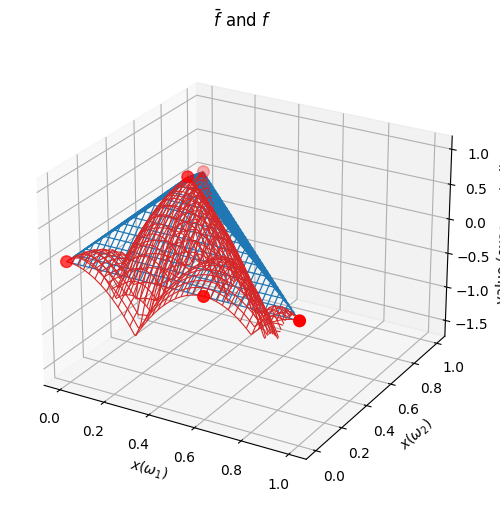
\includegraphics[scale=0.4]{mps-both.png}
\begin{original}
    \caption{$f$ and $\overline{f}$\label{fig:mps-both}}
\end{original}
\begin{translation}
    \caption{$f$与$\overline{f}$}
\end{translation}
  \end{subfigure}
  \qquad \qquad
  \begin{subfigure}[b]{0.35\textwidth}
    \centering
    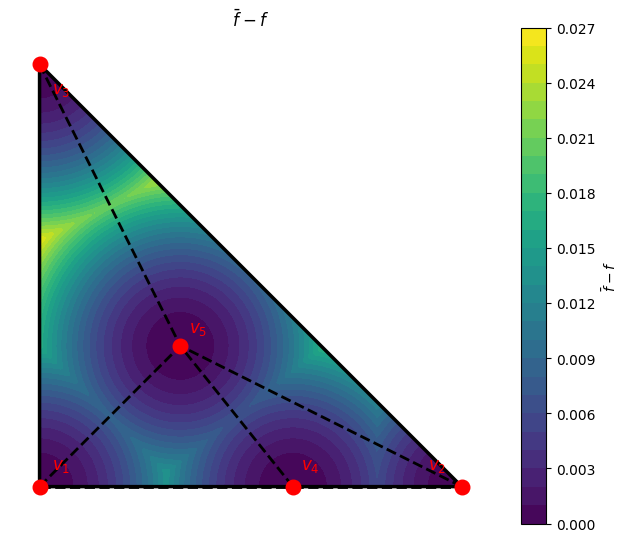
\includegraphics[scale=0.35]{mps-heat.png}
\begin{original}
    \caption{$\mathrm{supp}(\nu)$\label{fig:mps-heat}}
\end{original}
\begin{translation}
    \caption{$\mathrm{supp}(\nu)$}
\end{translation}
  \end{subfigure}
\begin{original}
  \caption{An exposed point $\nu$ of $\mathrm{MPS}(\mu)$}
\end{original}
\begin{translation}
  \caption{$\mathrm{MPS}(\mu)$的一个暴露点$\nu$}
\end{translation}
  \label{fig:mps-exposed}
\end{figure}

\begin{prop}[Exposed Points of Multidimensional MPS]\label{prop:mps}
\begin{original}
For any full-dimensional compact convex $X \subseteq \R^n$ and any $\mu \in \Delta(X)$ that is mutually absolutely continuous with respect to the Lebesgue measure, the following statements are equivalent:
\begin{itemize}
    \item[(a)] $\nu$ is an exposed point of $\emph{MPS}(\mu)$.
    \item[(b)] There exists a continuous $f$ with a strict contact and simplicial-touching affine envelope regions $S^{c}_{h^x}$ for a full-measure set of $x \in S^c$, and $\nu = P^f * \mu$, where $P^f(\,\cdot\,\mid x) = \delta_x$ for $x \in S$ and $P^f(\,\cdot\,\mid x)$ is the unique barycentric splitting for the full-measure set of $x \in S^c$.
\end{itemize}
\end{original}
\begin{translation}
对任意全维紧凸$X \subseteq \R^n$和任意与Lebesgue测度相互绝对连续的$\mu \in \Delta(X)$，以下陈述等价：
\begin{itemize}
    \item[(a)] $\nu$是$\emph{MPS}(\mu)$的暴露点。
    \item[(b)] 存在连续函数$f$具有严格接触和单形-接触的仿射包络区域$S^{c}_{h^x}$（对$S^c$的全测度子集$x$成立），且$\nu = P^f * \mu$，其中对$x \in S$有$P^f(\,\cdot\,\mid x) = \delta_x$，对$S^c$的全测度子集$x$有$P^f(\,\cdot\,\mid x)$是唯一重心分裂。
\end{itemize}
\end{translation}
\end{prop}

\begin{original}
\Cref{fig:mps-exposed} illustrates an exposed point $\nu$ of the set $\text{MPS}(\mu)$. \Cref{fig:mps-both} plots the associated exposing function $f$ (in red) and its concave envelope $\overline{f}$ (in blue), and marks the points where $\overline{f}=f$. It can be readily seen from \Cref{fig:mps-both} that $f$ has a strict contact and simplicial-touching affine envelope regions. \Cref{fig:mps-heat} plots the heat map of $\overline{f}-f$, and the dots correspond to the points where $\overline{f}=f$, which indicate the support of $\nu$.
\end{original}
\begin{translation}
\Cref{fig:mps-exposed}展示了$\text{MPS}(\mu)$的暴露点$\nu$。\Cref{fig:mps-both}绘制了相关的暴露函数$f$（红色）及其凹包络$\overline{f}$（蓝色），并标记了$\overline{f}=f$的点。从\Cref{fig:mps-both}可以清楚看出$f$具有严格接触和单形-接触的仿射包络区域。\Cref{fig:mps-heat}绘制了$\overline{f}-f$的热力图，圆点对应$\overline{f}=f$的点，表示$\nu$的支撑集。
\end{translation}

\begin{original}
An immediate consequence of \Cref{prop:mps} is that any exposed point of $\text{MPS}(\mu)$ takes the form of $P*\mu$, where the kernel $P$ has the property that either (i) it does not move the mass; or (ii) on a collection of non-overlapping simplices (e.g., triangles in $\R^2$), it splits each point in a simplex into the vertices of the simplex. This immediately generalizes the exposed point characterization of \citet*{kleiner2021extreme} in the one-dimensional case, where the convex regions are simply intervals.
\end{original}
\begin{translation}
\Cref{prop:mps}的一个直接推论是，$\text{MPS}(\mu)$的任何暴露点都具有$P*\mu$的形式，其中核$P$具有性质：要么(i)不移动质量；要么(ii)在一组不重叠的单纯形（例如$\R^2$中的三角形）上，它将单纯形中的每个点分裂为单纯形的顶点。这直接推广了\citet*{kleiner2021extreme}在一维情形中对暴露点的刻画，其中凸区域仅仅是区间。
\end{translation}

\paragraph{Multidimensional MPC.}\hspace{-2mm}
\begin{original}
Now, consider the orbit
\[\text{MPC}(\mu) := \big\{\nu: \mu \preceq_{\text{concave}} \nu\big\} = \big\{\nu: \nu \preceq_{\text{convex}} \mu \big\}\,.\]
Since the set of convex functions is not closed under pointwise minimum---it is closed under pointwise maximum---it follows that optimization involving $\text{MPC}(\mu)$ generally admits complex structures. For example, by \Cref{thm:main}, the value function $V^\star_f$ must be strictly concave on $\Delta(X)$ for some $f$. See \citet{kleiner2024extreme} for the characterization of the structure of Lipschitz exposed points of $\text{MPC}(\mu)$ for finitely-supported $\mu$.
\end{original}
\begin{translation}
现在考虑轨道$\text{MPC}(\mu) := \{\nu: \mu \preceq_{\text{concave}} \nu\} = \{\nu: \nu \preceq_{\text{convex}} \mu\}$。由于凸函数集在逐点最小值下不封闭——它在逐点最大值下封闭——由此，涉及$\text{MPC}(\mu)$的优化通常具有复杂的结构。例如，由\Cref{thm:main}，对某些$f$，值函数$V^\star_f$必须在$\Delta(X)$上严格凹。参见\citet{kleiner2024extreme}关于有限支撑$\mu$下$\text{MPC}(\mu)$的Lipschitz暴露点结构的刻画。
\end{translation}

\paragraph{Multidimensional Stochastic Dominance.}\hspace{-2mm}
\begin{original}
Let
\[\text{LSD}(\mu) := \big\{\nu: \nu \preceq_{\text{nondecreasing}} \mu\big\}\,,\]
where $\preceq_{\text{nondecreasing}}$ is the stochastic dominance order, i.e., $\C$ is the set of nondecreasing functions on $\R^n$. Similarly, let
\[\text{HSD}(\mu) := \big\{\nu:   \mu \preceq_{\text{nondecreasing}} \nu\big\} = \big\{\nu:   \nu \preceq_{\text{nonincreasing}} \mu\big\}\,.\]
Since both nondecreasing functions and nonincreasing functions are closed under pointwise minimum, by \Cref{thm:main}, optimization problems involving $\text{LSD}(\mu)$ and $\text{HSD}(\mu)$ admit simple structures---in particular, \Cref{cor:pointwise,cor:chain,cor:nested-optimization}  and \Cref{prop:exposed} immediately apply. Now, to illustrate, we apply \Cref{prop:exposed} to further characterize the exposed points of $\text{LSD}(\mu)$ and $\text{HSD}(\mu)$.
\end{original}
\begin{translation}
令$\text{LSD}(\mu) := \{\nu: \nu \preceq_{\text{nondecreasing}} \mu\}$，其中$\preceq_{\text{nondecreasing}}$是随机占优序，即$\C$是$\R^n$上非递减函数的集合。类似地，令$\text{HSD}(\mu) := \{\nu: \mu \preceq_{\text{nondecreasing}} \nu\} = \{\nu: \nu \preceq_{\text{nonincreasing}} \mu\}$。由于非递减函数和非递增函数在逐点最小值下都是封闭的，由\Cref{thm:main}，涉及$\text{LSD}(\mu)$和$\text{HSD}(\mu)$的优化问题具有简单结构——特别地，\Cref{cor:pointwise,cor:chain,cor:nested-optimization}和\Cref{prop:exposed}立即适用。现在，为作说明，我们应用\Cref{prop:exposed}来进一步刻画$\text{LSD}(\mu)$和$\text{HSD}(\mu)$的暴露点。
\end{translation}

\begin{original}
We start with $\text{LSD}(\mu)$. For any $f$, the $\C$-envelope $\overline{f}$ is simply the monotone envelope of $f$, i.e. $\overline{f}(x) = \max_{y \leq x} f(y)$. Define
\[S := \Big\{x: \overline{f}(x) = f(x)\Big\}\,.\]
For any $z \in \text{Ran}(\overline{f})$, let
\[R_z := \Big\{x: \overline{f}(x) = z\Big\}\,, \]
and
\[T_z := S \cap R_z = \Big\{x: \overline{f}(x) = f(x) = z\Big\}\,.\]
We say that $f$ has a \textit{\textbf{strict monotone contact}} if for a.e. $x \in S$, we have $f(x) > f(y)$ for all $y \leq x$ and $y \neq x$ (in the coordinatewise order). For any $z \in \text{Ran}(\overline{f})$, let
\[S^c_z:= R_z \cap S^c\,.\]
Clearly, $\{S^c_z\}_{z \in \text{Ran}(\overline{f})}$ is a partition of $S^c$. We write $z^x = \overline{f}(x)$. We refer to $\{S^c_z\}$ as \textit{\textbf{monotone envelope regions}}. We say a monotone envelope region $S^c_z$ is \textit{\textbf{downward staircase-like}} if there exists some upward-closed set $A_z \subset [0, 1]^n$ such that
\[R_z \backslash A_z = \biguplus_{\underline{x} \in T_z}\Big(\big\{\,x: x \geq \underline{x} \,\big\}\, \backslash \,A_z\Big) \,.\]
If $S^c_z$ is downward staircase-like, then for any $x \in R_z \backslash A_z$, there exists a unique \textit{\textbf{downward transport}} that deterministically transports $x$ to $\underline{x}$ for some $\underline{x} \in T_z$.
\end{original}
\begin{translation}
我们从$\text{LSD}(\mu)$开始。对任意$f$，$\C$-包络$\overline{f}$就是$f$的单调包络，即$\overline{f}(x) = \max_{y \leq x} f(y)$。定义$S := \{x: \overline{f}(x) = f(x)\}$。对任意$z \in \text{Ran}(\overline{f})$，令$R_z := \{x: \overline{f}(x) = z\}$，$T_z := S \cap R_z = \{x: \overline{f}(x) = f(x) = z\}$。我们称$f$具有\textit{\textbf{严格单调接触}}，如果对几乎每个$x \in S$，对所有$y \leq x$且$y \neq x$（按坐标序）有$f(x) > f(y)$。对任意$z \in \text{Ran}(\overline{f})$，令$S^c_z:= R_z \cap S^c$。显然$\{S^c_z\}_{z \in \text{Ran}(\overline{f})}$是$S^c$的一个划分。我们记$z^x = \overline{f}(x)$。我们称$\{S^c_z\}$为\textit{\textbf{单调包络区域}}。我们称单调包络区域$S^c_z$是\textit{\textbf{向下阶梯状}}的，如果存在某个向上封闭集$A_z \subset [0, 1]^n$使得$R_z \setminus A_z$是互不相交的集合$\{x: x \geq \underline{x}\} \setminus A_z$（$\underline{x} \in T_z$）的并。如果$S^c_z$是向下阶梯状的，则对任意$x \in R_z \setminus A_z$，存在唯一的\textit{\textbf{向下运输}}确定性地将$x$运输到某个$\underline{x} \in T_z$。
\end{translation}

\begin{prop}[Exposed Points of Multidimensional FOSD]\label{prop:fosd}
\begin{original}
For any $\mu \in \Delta([0, 1]^n)$ that is mutually absolutely continuous with respect to the Lebesgue measure, the following statements are equivalent:
\begin{itemize}
    \item[(a)] $\nu$ is an exposed point of $\emph{LSD}(\mu)$.
    \item[(b)] There exists a continuous $f$ with a strict monotone contact and downward staircase-like monotone envelope regions $S^{c}_{z^x}$ for a full-measure set of $x \in S^c$ with $x \in R_{z^x}\backslash A_{z^x}$, and $\nu = P^f * \mu$, where $P^f(\,\cdot\,\mid x) = \delta_x$ for $x \in S$ and $P^f(\,\cdot\,\mid x)$ is the unique downward transport for the full-measure set of $x \in S^c$.
\end{itemize}
\end{original}
\begin{translation}
对任意与Lebesgue测度相互绝对连续的$\mu \in \Delta([0, 1]^n)$，以下陈述等价：
\begin{itemize}
    \item[(a)] $\nu$是$\emph{LSD}(\mu)$的暴露点。
    \item[(b)] 存在连续函数$f$具有严格单调接触和向下阶梯状的单调包络区域$S^{c}_{z^x}$（对$S^c$中满足$x \in R_{z^x}\setminus A_{z^x}$的全测度子集$x$成立），且$\nu = P^f * \mu$，其中对$x \in S$有$P^f(\,\cdot\,\mid x) = \delta_x$，对$S^c$的全测度子集$x$有$P^f(\,\cdot\,\mid x)$是唯一向下运输。
\end{itemize}
\end{translation}
\end{prop}

\begin{figure}[t]
  \begin{subfigure}[b]{0.45\textwidth}
    \centering
    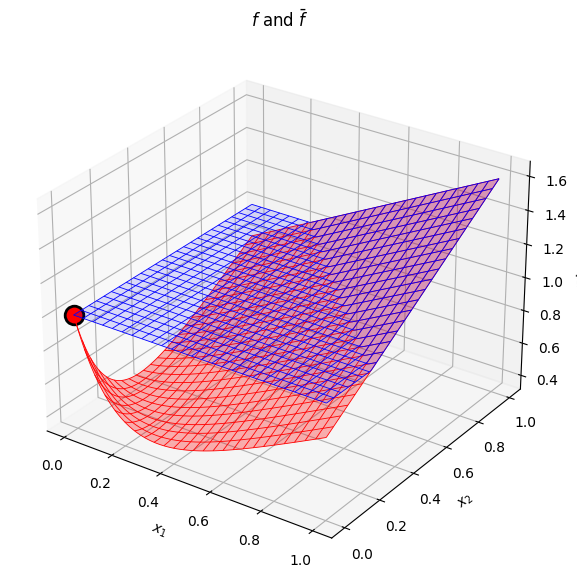
\includegraphics[scale=0.3]{fosd-both.png}
\begin{original}
    \caption{$f$ and $\overline{f}$\label{fig:fosd-both}}
\end{original}
\begin{translation}
    \caption{$f$与$\overline{f}$}
\end{translation}
  \end{subfigure}
  \quad
  \begin{subfigure}[b]{0.45\textwidth}
    \centering
    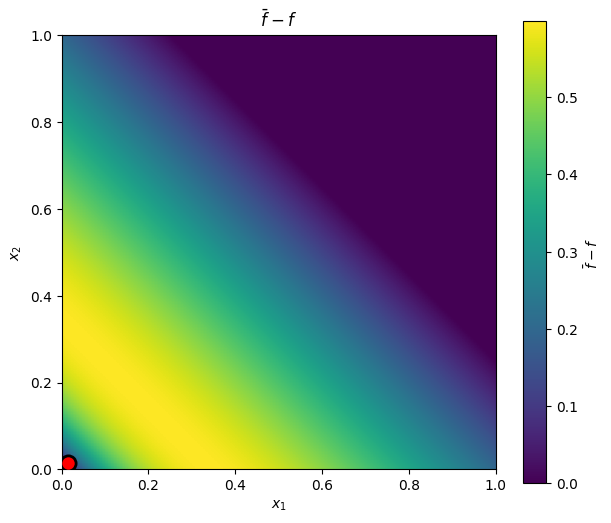
\includegraphics[scale=0.3]{fosd-heat.png}
\begin{original}
    \caption{$\mathrm{supp}(\nu)$\label{fig:fosd-heat}}
\end{original}
\begin{translation}
    \caption{$\mathrm{supp}(\nu)$}
\end{translation}
  \end{subfigure}
\begin{original}
  \caption{An exposed point $\nu$ of $\mathrm{LSD}(\mu)$}
\end{original}
\begin{translation}
  \caption{$\mathrm{LSD}(\mu)$的一个暴露点$\nu$}
\end{translation}
  \label{fig:fosd-exposed}
\end{figure}

\begin{original}
\Cref{fig:fosd-exposed} illustrates an exposed point $\nu$ of $\text{LSD}(\mu)$. \Cref{fig:fosd-both} plots the associated exposing function $f$ and its monotone envelope $\overline{f}$. It can be seen from \Cref{fig:fosd-both} that $f$ has a strict monotone contact. \Cref{fig:fosd-heat} plots the heat map of $\overline{f}-f$. The region where $\overline{f}=f$ consists of the point $(0,0)$ and the top-right corner. Every point not in this region has a unique downward transport to $(0,0)$.

An immediate consequence of \Cref{prop:fosd} is that any exposed point of $\text{LSD}(\mu)$ takes the form of $P*\mu$, where the kernel $P$ has the property that either (i) it does not move the mass; or (ii) on a collection of non-overlapping differences of two nested upsets that are downward staircase-like, it transports each point in any such region down to a corresponding unique minimal element. This immediately generalizes the exposed point characterization of \citet{yang2024monotone} in the one-dimensional case, where the differences of two nested upsets are simply intervals.

The case of $\text{HSD}(\mu)$ is exactly symmetric to $\text{LSD}(\mu)$, in contrast to the asymmetry that arises between $\text{MPS}(\mu)$ and $\text{MPC}(\mu)$. In particular, it can be characterized symmetrically by using \textit{\textbf{decreasing envelope regions}}, the differences of nested downward-closed sets that form \textit{\textbf{upward staircase-like}} shapes, and the \textit{\textbf{upward transport}} maps. We omit the details here.
\end{original}
\begin{translation}
\Cref{fig:fosd-exposed}展示了$\text{LSD}(\mu)$的暴露点$\nu$。\Cref{fig:fosd-both}绘制了相关的暴露函数$f$及其单调包络$\overline{f}$。从\Cref{fig:fosd-both}可以看出$f$具有严格单调接触。\Cref{fig:fosd-heat}绘制了$\overline{f}-f$的热力图。$\overline{f}=f$的区域由点$(0,0)$和右上角组成。不在该区域的每个点都有唯一的向下运输到$(0,0)$。

\Cref{prop:fosd}的一个直接推论是，$\text{LSD}(\mu)$的任何暴露点都具有$P*\mu$的形式，其中核$P$具有性质：要么(i)不移动质量；要么(ii)在一组不重叠的两个嵌套上集的差（呈向下阶梯状）上，它将每个点运输到对应的唯一极小元素。这直接推广了\citet{yang2024monotone}在一维情形中对暴露点的刻画，其中两个嵌套上集的差仅仅是区间。

$\text{HSD}(\mu)$的情形与$\text{LSD}(\mu)$完全对称，这与$\text{MPS}(\mu)$和$\text{MPC}(\mu)$之间出现的不对称形成对比。特别地，它可以通过使用\textit{\textbf{递减包络区域}}、形成\textit{\textbf{向上阶梯状}}形状的嵌套向下闭集的差以及\textit{\textbf{向上运输}}映射来对称地刻画。我们在此省略细节。
\end{translation}

\section{Consistent Comparisons of Experiments}\label{sec:compare}
\begin{original}
In this section, we apply our main characterization to generalize Blackwell's theorem. In a pioneering paper, \citet{Blackwell1951Comparison} identifies an order on experiments that has a dual representation. On the one hand, the Blackwell order has an instrumental-value-based representation: an experiment Blackwell dominates another if and only if one yields a higher value under \emph{all} statistical decision problems than the other. On the other hand, the Blackwell order has an information-technology-based interpretation: an experiment Blackwell dominates another if and only if one can be obtained by adding noise to (i.e., garbling) the other. In the space of distributions of posterior beliefs induced by an experiment under a given prior, this dual representation essentially identifies an order $\preceq$ over $\Delta(X)$, a convex cone of test functions (i.e., a class of problems) $\C$, and a set of information technologies $\Pc$, such that the order $\preceq$ can be simultaneously represented by comparing values of problems $g \in \C$, as well as being coupled by some information technologies $P \in \Pc$. In this regard, Blackwell's theorem identifies such an order where $\C$ is the set of convex functions and $\Pc$ is the set of martingales.
\end{original}
\begin{translation}
在本节中，我们将主要刻画应用于推广Blackwell定理。在一篇开创性论文中，\citet{Blackwell1951Comparison}识别了实验上的一个具有双重表示的序。一方面，Blackwell序具有基于工具价值的表示：一个实验Blackwell支配另一个实验，当且仅当前者在所有统计决策问题下比后者产生更高的价值。另一方面，Blackwell序具有基于信息技术的解释：一个实验Blackwell支配另一个实验，当且仅当前者可以通过向后者添加噪声（即garbling）获得。在给定先验下实验诱导的后验信念分布空间中，这种双重表示本质上识别了$\Delta(X)$上的一个序$\preceq$、一个检验函数凸锥（即一类问题）$\C$和一组信息技术$\Pc$，使得序$\preceq$可以同时通过比较问题$g \in \C$的值来表示，以及通过某些信息技术$P \in \Pc$耦合来表示。就此而言，Blackwell定理识别了这样一个序，其中$\C$是凸函数集，$\Pc$是鞅的集合。
\end{translation}

\begin{original}
Given Blackwell's theorem, one natural question is: in general, which orders $\preceq$ over $\Delta(X)$ admit such dual representations? When is it the case that an abstract order $\preceq$ over $\Delta(X)$ can be simultaneously interpreted as an order that reflects instrumental values, as well as an order that reflects the information content of distributions over posterior beliefs? In this section, we characterize all such orders. To begin with, we first introduce some notation and terminology.
\end{original}
\begin{translation}
给定Blackwell定理，一个自然的问题是：一般来说，$\Delta(X)$上的哪些序$\preceq$允许这样的双重表示？何时一个抽象的序$\preceq$可以同时被解释为反映工具价值的序，以及反映后验信念分布信息内容的序？在本节中，我们刻画了所有此类序。首先，我们引入一些符号和术语。
\end{translation}

\begin{original}
Throughout this section, fix a compact Polish state space $\Omega$, and let $X := \Delta(\Omega)$ be the space of beliefs over $\Omega$. Let $\C_0$ be the set of bounded lower semicontinuous functions on $X$ and $\Pc_0$ be the set of measurable Markov kernels. For any $\Pc \subseteq \Pc_0$ and for any $x \in X$, let
\[
\Pc_x:=\Big\{P(\,\cdot\,\mid x): P \in \Pc \Big\}\,.
\]
We say that $\Pc \subseteq \Pc_0$ is \textit{\textbf{rectangular}} if $P \in \Pc$ whenever $P(\,\cdot\,\mid x) \in \Pc_x$ for all $x \in X$. We say that a pair $(\C,\Pc)$ is \textit{\textbf{regular}} if $\C \subseteq \C_0$ is a convex cone such that $\C \cap C(X)$ is sup-norm closed, contains all constant functions, admits continuous approximations from below, and is closed under bounded increasing pointwise limits; while $\Pc \subseteq \Pc_0$ has a closed graph,\footnote{That is, the graph $\{(x,\eta): x\in X\,,\, \eta \in \mathcal{P}_x\}$ is closed in $X \times \Delta(X)$.} contains the identity kernel, and is convex and rectangular. We impose regularity on $(\C,\Pc)$ throughout this section unless stated otherwise.
\end{original}
\begin{translation}
在本节中，固定一个紧Polish状态空间$\Omega$，令$X := \Delta(\Omega)$为$\Omega$上的信念空间。令$\C_0$为$X$上有界下半连续函数的集合，$\Pc_0$为可测Markov核的集合。对任意$\Pc \subseteq \Pc_0$和任意$x \in X$，令$\Pc_x:=\{P(\,\cdot\,\mid x): P \in \Pc\}$。我们称$\Pc \subseteq \Pc_0$是\textit{\textbf{矩形}}的，如果当对所有$x \in X$有$P(\,\cdot\,\mid x) \in \Pc_x$时就有$P \in \Pc$。我们称一对$(\C,\Pc)$是\textit{\textbf{正则}}的，如果$\C \subseteq \C_0$是一个凸锥，满足$\C \cap C(X)$在上确界范数下封闭、包含所有常数函数、允许从下方的连续逼近，且在有界递增逐点极限下封闭；而$\Pc \subseteq \Pc_0$具有闭图、\footnote{即图$\{(x,\eta): x\in X, \eta \in \mathcal{P}_x\}$在$X \times \Delta(X)$中是闭的。}包含恒等核，且是凸和矩形的。除非另有说明，在整节中我们对$(\C,\Pc)$施加正则性条件。
\end{translation}

\begin{original}
For any $\C$, define the following comparison:
\[\mu \preceq_{\C} \nu \,\,\text{ if }\,\, \int g(x) \nu(\d x) \geq \int g(x) \mu( \d x)\,, \forall\, g \in \C\,. \eqtag[-2.5em][0.6\baselineskip]{\textbf{Value Description}}{eq:payoff}\]
For any $\Pc$, define the following comparison:
\[\mu \preceq^{\Pc} \nu \,\,\text{ if }\,\, \exists \, P \in \Pc \text{ s.t. } \nu = P * \mu\,. \eqtag[-2.5em][0.2\baselineskip]{\textbf{Information Description}}{eq:information} \]
For any order $\preceq$ on $\Delta(X)$, we say that $\preceq$ is \textit{\textbf{Blackwell-consistent}} if there exists some (regular) $(\C, \Pc)$ such that
\[\preceq_{\C} \,= \,\preceq \,= \, \preceq^\mathcal{P}\,, \eqtag[-2.5em][0.2\baselineskip]{\textbf{Blackwell Consistency}}{eq:blackwell-consistency}\]
in which case we call $(\C, \Pc)$ a \textit{\textbf{Blackwell-consistent pair}}.
\end{original}
\begin{translation}
对任意$\C$，定义以下比较：
\[\mu \preceq_{\C} \nu \,\,\text{ 如果 }\,\, \int g(x) \nu(\d x) \geq \int g(x) \mu( \d x)\,, \forall\, g \in \C\,. \eqtag[-2.5em][0.6\baselineskip]{\textbf{价值描述}}{eq:payoff}\]
对任意$\Pc$，定义以下比较：
\[\mu \preceq^{\Pc} \nu \,\,\text{ 如果 }\,\, \exists \, P \in \Pc \text{ s.t. } \nu = P * \mu\,. \eqtag[-2.5em][0.2\baselineskip]{\textbf{信息描述}}{eq:information} \]
对$\Delta(X)$上的任意序$\preceq$，我们称$\preceq$是\textit{\textbf{Blackwell-一致的}}，如果存在某个（正则的）$(\C, \Pc)$使得
\[\preceq_{\C} \,= \,\preceq \,= \, \preceq^\mathcal{P}\,, \eqtag[-2.5em][0.2\baselineskip]{\textbf{Blackwell一致性}}{eq:blackwell-consistency}\]
此时我们称$(\C, \Pc)$为\textit{\textbf{Blackwell-一致对}}。
\end{translation}

\begin{original}
We say that $\C$ is \textit{\textbf{max-closed}} if for any $g_1,g_2 \in \C$, $\max\{g_1,g_2\} \in \C$. As an immediate consequence of \Cref{thm:main}, our next result characterizes all Blackwell-consistent orders:
\end{original}
\begin{translation}
我们称$\C$是\textit{\textbf{最大-封闭}}的，如果对任意$g_1,g_2 \in \C$有$\max\{g_1,g_2\} \in \C$。作为\Cref{thm:main}的直接推论，我们的下一个结果刻画了所有Blackwell-一致序：
\end{translation}

\begin{theorem}\label{thm:main2}
\begin{original}
An order $\preceq$ is Blackwell-consistent if and only if $\preceq = \preceq_\C$ for a max-closed $\C$.
\end{original}
\begin{translation}
一个序$\preceq$是Blackwell-一致的当且仅当$\preceq = \preceq_\C$对某个最大-封闭的$\C$成立。
\end{translation}
\end{theorem}
\begin{proof}[Proof of \Cref{thm:main2}]
\begin{original}
\textbf{The ``if'' direction:} Suppose $\preceq = \preceq_\C$ for a max-closed $\C$. Let
\[\Pc := \Big\{P \in \Pc_0: \delta_x \preceq_\C  P *\delta_x \text{ for all $x$} \Big\}\,.\]
Note that $\mu\preceq \nu \iff \nu \preceq_{[-\C]} \mu$ where $[-\C]$ is a convex cone that is min-closed. Thus, for any $\mu\preceq \nu$, by \Cref{thm:main},\footnote{It can be verified that the technical assumptions required by \Cref{thm:main} hold for $[-\C]$ if $\C$ is regular.}  there exists some $P$ such that $\nu = P * \mu$ where $P * \delta_x  \preceq_{[-\C]} \delta_x$, i.e., $\delta_x \preceq_{\C} P * \delta_x$ for all $x$, and hence $P \in \Pc$.  Therefore, $\preceq_\C \implies \preceq^\Pc$. Moreover, for any $\nu = P * \mu$ for some $P \in \Pc$, since $\preceq_\C$ is an integral stochastic order and $\delta_x \preceq_\C P * \delta_x$ for all $x$, it follows immediately that $\mu \preceq_\C \nu$. Thus, $\preceq^\Pc \implies \preceq_\C$ and hence these two are equivalent. Thus, $\preceq$ is Blackwell-consistent.\footnote{It can be verified that the constructed $\Pc$ is regular; see \Cref{lem:basic} in the appendix.}

\textbf{The ``only if'' direction:} Suppose $\preceq$ is Blackwell-consistent. Then there exists some regular $(\C, \Pc)$ such that $\preceq_\C = \preceq = \preceq^\Pc$. We claim that $\preceq_{[-\C]}$ admits order-preserving couplings. Indeed, fix any $\nu \preceq_{[-\C]} \mu$. Then, $\mu \preceq_{\C} \nu$ and hence $\nu = P * \mu$ for some $P \in \Pc$. For any $x$, note that by definition $\delta_x \preceq^{\Pc} P * \delta_x$ and hence $\delta_x \preceq_\C P * \delta_x$ by Blackwell consistency. Thus, for all $x \in X$ and all $g \in \C$, we have
\[\int g(y) P(\d y\mid x) \geq g(x)\]
and hence
\[\int [-g](y) P(\d y\mid x) \leq [-g](x)\,.\]
Thus, $P * \delta_x \preceq_{[-\C]} \delta_x$ for all $x$. Therefore, $\preceq_{[-\C]}$ admits order-preserving couplings. By \Cref{thm:main}, $[-\C]$ is min-closed and hence $\C$ is max-closed, as desired.
\end{original}
\begin{translation}
\textbf{``如果''方向：}假设对最大-封闭的$\C$有$\preceq = \preceq_\C$。令$\Pc := \{P \in \Pc_0: \delta_x \preceq_\C P *\delta_x,\ \forall x\}$。注意$\mu\preceq \nu \iff \nu \preceq_{[-\C]} \mu$，其中$[-\C]$是最小-封闭的凸锥。因此，对任意$\mu\preceq \nu$，由\Cref{thm:main}存在$P$使得$\nu = P * \mu$，且$P * \delta_x \preceq_{[-\C]} \delta_x$即$\delta_x \preceq_{\C} P * \delta_x$，故$P \in \Pc$。由此$\preceq_\C \implies \preceq^\Pc$。反之，对任意$\nu = P * \mu$，$P \in \Pc$，由积分随机序定义有$\mu \preceq_\C \nu$，即$\preceq^\Pc \implies \preceq_\C$。二者等价，故$\preceq$是Blackwell-一致的。

\textbf{``仅当''方向：}假设$\preceq$是Blackwell-一致的。则存在正则$(\C, \Pc)$使得$\preceq_\C = \preceq = \preceq^\Pc$。我们断言$\preceq_{[-\C]}$存在保序耦合。固定任意$\nu \preceq_{[-\C]} \mu$，即$\mu \preceq_{\C} \nu$，故存在$P \in \Pc$使得$\nu = P * \mu$。对任意$x$，由定义有$\delta_x \preceq^{\Pc} P * \delta_x$，由Blackwell一致性有$\delta_x \preceq_\C P * \delta_x$。因此对所有$x$和$g \in \C$有$\int g(y) P(\d y\mid x) \geq g(x)$，从而$\int [-g](y) P(\d y\mid x) \leq [-g](x)$，即$P * \delta_x \preceq_{[-\C]} \delta_x$。故$\preceq_{[-\C]}$存在保序耦合。由\Cref{thm:main}，$[-\C]$是最小-封闭的，故$\C$是最大-封闭的。
\end{translation}
\end{proof}

\begin{original}
\Cref{thm:main2} asserts that $\preceq$ is Blackwell-consistent---admitting simultaneous value-based and information-based representations---if and only if the class of test functions $\C$ in its value description is closed under pointwise maximum. Intuitively, it means that whenever $g_1, g_2 \in \C$ are two problems, the problem whose value at each posterior belief $x$ is $\max\{g_1(x), g_2(x)\}$---corresponding to choosing the better of the two problems at each belief---must also belong to $\C$. This ``choose the better problem'' closure property turns out to be the \textit{exact} condition that bridges the value-based and information-based descriptions of an order.

Now, a few natural questions arise. What is the key structure of $\Pc$ in the dual space that mirrors the max-closure property of $\C$? Which pairs $(\C, \Pc)$ are consistent? Given a Blackwell-consistent order, are there multiple pairs $(\C, \Pc)$ that represent the same order? We now answer all of them in our next result.
\end{original}
\begin{translation}
\Cref{thm:main2}断言$\preceq$是Blackwell-一致的——允许同时具有基于价值和基于信息的表示——当且仅当其价值描述中的检验函数类$\C$在逐点最大值下封闭。直观上，这意味着每当$g_1, g_2 \in \C$是两个问题，则其值在每个后验信念$x$处为$\max\{g_1(x), g_2(x)\}$的问题——对应在每个信念处选择两个问题中较好的一个——也必须属于$\C$。这一``选择更好问题''的封闭性质恰好是连接一个序的基于价值和基于信息描述的\textit{精确}条件。

现在，出现了几个自然的问题。$\Pc$在对偶空间中的什么关键结构与$\C$的最大-封闭性质相对应？哪些对$(\C, \Pc)$是一致的？给定一个Blackwell-一致序，是否存在多个$(\C, \Pc)$表示同一个序？我们现于下一个结果中回答所有这些问题。
\end{translation}

\begin{original}
For any $P_1,P_2 \in \Pc_0$, recall from \weqref{\textbf{Composition}}{eq:composition} that $P_1 \circ P_2$ denotes the composition of the two kernels. We say that $\Pc \subseteq \Pc_0$ is \textit{\textbf{composition-closed}} if for any $P_1,P_2 \in \Pc$, $P_1\circ P_2 \in \Pc$. As we show, it turns out that composition-closure property of $\Pc$ is the \textit{exact} condition that mirrors the max-closure property of $\C$, each of which is equivalent to Blackwell consistency.

To characterize the consistent pairs, we build on the construction given in the proof of \Cref{thm:main2}. To start, recall the notation from \weqref{\textbf{Conditional Expectation}}{eq:conditional-expectation}, $[g*P](x) := \int g(y) P(\d y \mid x)$. Define two operators $\Phi$ and $\Psi$ as follows: For any $\C \subseteq \C_0$, let
\[
\Psi(\C):=\Big\{P \in \Pc_0: g*P \geq g\,, \, \, \forall\, g \in \C\Big\}\, \eqtag[-2.5em]{\textbf{Improving Kernels}}{eq:improving-kernels}
\]
denote the set of belief transitions that are uniformly improving across all test functions in $\C$. For any $\Pc \subseteq \Pc_0$, let
\[
\Phi(\Pc):=\Big\{g \in \C_0: g*P \geq g\,, \, \, \forall\, P \in \Pc\Big\}\, \eqtag[-2.5em]{\textbf{Improving Utilities}}{eq:improving-utilities}
\]
denote the set of test functions that are uniformly improving across all belief transitions in $\Pc$. We say that $(\C, \Pc)$ is \textit{\textbf{Blackwell-invariant}} if
\[ \Psi(\C)=\Pc  \text{ and } \Phi(\Pc)=\C \eqtag[-2.5em][0.2\baselineskip]{\textbf{Blackwell Invariance}}{eq:blackwell-invariance}\,.\]
A Blackwell-invariant pair $(\C,\Pc)$ has a straightforward interpretation. It means that the available information technologies $\Pc$ are exactly the ones that are valuable for problems in $\C$ (i.e., $\Pc=\Psi(\C)$). In the meantime, the problems $\C$ are exactly the ones for which the available information technologies $\Pc$ are valuable (i.e., $\C=\Phi(\Pc)$).

Finally, we say that $\mathcal{P}$ is \textit{\textbf{one-shot sufficient}} if for all $f$ and all $x$, we have
\[\sup_{P \in \mathcal{P}} \int f(y) P(\d y \mid x) = \sup_{P \in \mathcal{P} \otimes \mathcal{P}} \int f(y) P(\d y \mid x), \eqtag[-2.5em][0.6\baselineskip]{\textbf{One Shot}}{eq:one-shot-sufficient} \]
where
\[
\Pc \otimes \Pc:=\{P_1 \circ P_2: P_1,P_2 \in \Pc\}
\]
denotes the set of all (twice) compositions of elements in $\Pc$. It is clear that if $\mathcal{P}$ is composition-closed, then it is one-shot sufficient.

In the case of the Blackwell order, $\C$ is the cone of convex functions and $\Pc$ is the set of martingale transition kernels. Clearly, $\C$ is max-closed and $\Pc$ is composition-closed. Moreover, $\Psi(\mathcal{C}) = \Pc$ and  $\Phi(\Pc) = \mathcal{C}$. That is, the test functions $\C$ and transition kernels $\Pc$ associated with the Blackwell order are in fact Blackwell-invariant. This turns out not to be a coincidence. Our next result shows that (i) the composition-closure property of $\Pc$ mirrors the max-closure property of $\C$, each of which characterizes Blackwell consistency, and (ii) Blackwell consistency is equivalent to Blackwell invariance, which turns out to be also equivalent to the one-shot sufficiency property of the set of transition kernels for optimization problems.

In general, different convex cones $\C$ and $\C'$ or different sets of kernels $\Pc$ and $\Pc'$ might induce the same comparisons, i.e., $\preceq_\C=\preceq_{\C'}$ or $\preceq^{\Pc}=\preceq^{\Pc'}$. Since Blackwell consistency is only a property about the induced order, one might naturally expect that there might be multiplicity involved in determining the consistent pairs. However, perhaps surprisingly, every Blackwell-consistent order admits a \textit{\textbf{unique}} consistent pair that characterizes it.
\end{original}
\begin{translation}
对任意$P_1,P_2 \in \Pc_0$，回顾\weqref{\textbf{Composition}}{eq:composition}中$P_1 \circ P_2$表示两个核的复合。我们称$\Pc \subseteq \Pc_0$是\textit{\textbf{复合-封闭}}的，如果对任意$P_1,P_2 \in \Pc$有$P_1\circ P_2 \in \Pc$。如我们所示，$\Pc$的复合-封闭性质恰好是与$\C$的最大-封闭性质相对应的\textit{精确}条件，两者都等价于Blackwell一致性。

为刻画一致对，我们在\Cref{thm:main2}证明中的构造基础上展开。定义两个算子$\Phi$和$\Psi$：对任意$\C \subseteq \C_0$，令$\Psi(\C):=\{P \in \Pc_0: g*P \geq g, \forall g \in \C\}$为在$\C$中所有检验函数下一致改善的信念转移集合。对任意$\Pc \subseteq \Pc_0$，令$\Phi(\Pc):=\{g \in \C_0: g*P \geq g, \forall P \in \Pc\}$为在$\Pc$中所有信念转移下一致改善的检验函数集合。我们称$(\C, \Pc)$是\textit{\textbf{Blackwell-不变的}}，如果$\Psi(\C)=\Pc$且$\Phi(\Pc)=\C$。Blackwell-不变对$(\C,\Pc)$有直接的解释：可用信息技术$\Pc$恰好是对$\C$中的问题有价值的技术（即$\Pc=\Psi(\C)$）；同时，问题$\C$恰好是可用信息技术$\Pc$对其有价值的问题（即$\C=\Phi(\Pc)$）。

最后，我们称$\mathcal{P}$是\textit{\textbf{一次性充分的}}，如果对所有$f$和所有$x$有$\sup_{P \in \mathcal{P}} \int f(y) P(\d y \mid x) = \sup_{P \in \mathcal{P} \otimes \mathcal{P}} \int f(y) P(\d y \mid x)$，其中$\Pc \otimes \Pc:=\{P_1 \circ P_2: P_1,P_2 \in \Pc\}$表示$\Pc$中元素的所有（二次）复合的集合。显然，如果$\mathcal{P}$是复合-封闭的，则它是一次性充分的。

在Blackwell序的情形中，$\C$是凸函数的锥，$\Pc$是鞅转移核的集合。显然，$\C$是最大-封闭的，$\Pc$是复合-封闭的。而且，$\Psi(\mathcal{C}) = \Pc$和$\Phi(\Pc) = \mathcal{C}$。即与Blackwell序相关的检验函数$\C$和转移核$\Pc$实际上是Blackwell-不变的。这并非巧合。我们的下一个结果表明：(i) $\Pc$的复合-封闭性质与$\C$的最大-封闭性质相对应，两者各自刻画了Blackwell一致性；(ii) Blackwell一致性等价于Blackwell不变性，后者也等价于转移核集合对优化问题的一次性充分性质。

一般来说，不同的凸锥$\C$和$\C'$或不同的核集合$\Pc$和$\Pc'$可能诱导相同的比较，即$\preceq_\C=\preceq_{\C'}$或$\preceq^{\Pc}=\preceq^{\Pc'}$。由于Blackwell一致性只是关于诱导序的一个性质，人们可能自然预期在确定一致对时会涉及多重性。然而，也许令人惊讶的是，每个Blackwell-一致序有\textit{\textbf{唯一的}}一致对来刻画它。
\end{translation}

\begin{theorem}[Blackwell-Consistent Pairs]\label{thm:main-compare}
\begin{original}
The following are equivalent:
\begin{itemize}
    \item[(a)] $(\C, \Pc)$ is Blackwell-consistent.
    \item[(b)] $(\C, \Pc)$ is Blackwell-invariant.
    \item[(c)] $\Pc$ is one-shot sufficient, and $\C = \Phi(\Pc)$.
    \item[(d)] $\Pc$ is composition-closed, and $\C = \Phi(\Pc)$.
    \item[(e)] $\mathcal{C}$ is max-closed, and $\mathcal{P} = \Psi(\C)$.
    \end{itemize}
Moreover, every Blackwell-consistent order $\preceq$ admits a unique consistent pair $(\C, \Pc)$.
\end{original}
\begin{translation}
以下命题等价：
\begin{itemize}
    \item[(a)] $(\C, \Pc)$是Blackwell-一致的。
    \item[(b)] $(\C, \Pc)$是Blackwell-不变的。
    \item[(c)] $\Pc$是一次性充分的，且$\C = \Phi(\Pc)$。
    \item[(d)] $\Pc$是复合-封闭的，且$\C = \Phi(\Pc)$。
    \item[(e)] $\mathcal{C}$是最大-封闭的，且$\mathcal{P} = \Psi(\C)$。
    \end{itemize}
此外，每个Blackwell-一致序$\preceq$有唯一的一致对$(\C, \Pc)$。
\end{translation}
\end{theorem}


\subsection{Which Orders are Consistent under Bayesian Updating?}\label{sec:Bayes-plausible}
\begin{original}
With \Cref{thm:main2} and \Cref{thm:main-compare},  we now further specialize to Blackwell's environment, and characterize which orders of Blackwell experiments are Blackwell-consistent. Clearly, if beliefs are updated via Bayes' rule, then by Blackwell's theorem, the Blackwell order is Blackwell-consistent. We characterize all orders of Blackwell experiments that are Blackwell-consistent when beliefs are updated via Bayes' rule in this section, and characterize all updating rules that admit Blackwell-consistent orders in the next section.
\end{original}
\begin{translation}
有了\Cref{thm:main2}和\Cref{thm:main-compare}，我们现在进一步专门讨论Blackwell的环境，并刻画哪些Blackwell实验的序是Blackwell-一致的。显然，如果信念通过贝叶斯法则更新，那么由Blackwell定理，Blackwell序是Blackwell-一致的。我们在本节刻画当信念通过贝叶斯法则更新时所有Blackwell-一致的Blackwell实验序，并在下一节刻画所有允许Blackwell-一致序的更新规则。
\end{translation}

\subsubsection{Bayes-Plausible and Blackwell-Consistent Orders}
\begin{original}
To begin with, we say that an order $\preceq$ on $\Delta(X)$ is \textit{\textbf{Bayes-plausible}} if
\[\mu \preceq \nu \implies \int x \mu(\d x) = \int x \nu(\d x)\, \eqtag[-2.5em]{\textbf{Bayes Plausibility}}{eq:bayes-plausible}\,,\]
where the integral is in the sense of the Pettis integral, i.e., the two belief distributions must have the same barycenter.

An immediate consequence of \Cref{thm:main2} is the following:
\end{original}
\begin{translation}
首先，我们称$\Delta(X)$上的一个序$\preceq$是\textit{\textbf{贝叶斯-可信}}的，如果$\mu \preceq \nu \implies \int x \mu(\d x) = \int x \nu(\d x)$，其中积分是在Pettis积分的意义上，即两个信念分布必须有相同的重心。

\Cref{thm:main2}的一个直接推论如下：
\end{translation}

\begin{cor}\label{cor:blackwell-consistent-orders}
\begin{original}
For any pair $(\C, \Pc)$, the following are equivalent:
\begin{itemize}
    \item[(a)] $\preceq_\C = \preceq^\Pc$ is Bayes-plausible.
    \item[(b)] $\C$ is a max-closed superset of all
    convex functions, and $\Pc = \Psi(\C)$.
    \item[(c)] $\Pc$ is a composition-closed subset of
    all martingale kernels, and $\C = \Phi(\Pc)$.
\end{itemize}
In particular, any Bayes-plausible and Blackwell-consistent order strengthens the Blackwell order, and the Blackwell
order is the weakest such order.
\end{original}
\begin{translation}
对任意对$(\C, \Pc)$，以下命题等价：
\begin{itemize}
    \item[(a)] $\preceq_\C = \preceq^\Pc$是贝叶斯-可信的。
    \item[(b)] $\C$是所有凸函数的一个最大-封闭超集，且$\Pc = \Psi(\C)$。
    \item[(c)] $\Pc$是所有鞅核的一个复合-封闭子集，且$\C = \Phi(\Pc)$。
\end{itemize}
特别地，任何贝叶斯-可信且Blackwell-一致的序加强了Blackwell序，且Blackwell序是最弱的此类序。
\end{translation}
\end{cor}

\begin{original}
Indeed, \Cref{cor:blackwell-consistent-orders} follows because Bayes plausibility implies that all affine functions must be in the cone of test functions, which combined with \Cref{thm:main2} and \Cref{thm:main-compare} implies that all convex functions must be in the test cone since the test cone must be max-closed and any convex function is a pointwise supremum of a collection of affine functions. Therefore, any Bayes-plausible weakening of the Blackwell order through a subset of convex functions, such as the Lehmann order (\citealt{Lehmann}) or the linear convex order (\citealt{chen2025experiments}), cannot be consistent in our sense.\footnote{It is immediate to verify that neither of these orders is defined by a set of test functions that is max-closed.} \Cref{cor:blackwell-consistent-orders} shows that any Bayes-plausible and Blackwell-consistent order $\preceq$ must imply the Blackwell order---therefore, the Blackwell order is necessary for a consistent comparison, while maintaining Bayes plausibility.  In other words, any Bayes-plausible, Blackwell-consistent order $\preceq$ must rely on a set $\C$ of problems that includes all decision problems, and on a set $\Pc$ of information technologies that is a subset of martingales.
\end{original}
\begin{translation}
事实上，\Cref{cor:blackwell-consistent-orders}成立是因为贝叶斯可信性意味着所有仿射函数必须在检验函数锥中，结合\Cref{thm:main2}和\Cref{thm:main-compare}，这意味着所有凸函数必须在检验锥中，因为检验锥必须是最大-封闭的，且任何凸函数是一族仿射函数的逐点上确界。因此，通过凸函数子集对Blackwell序的任何贝叶斯-可信弱化，如Lehmann序(\citealt{Lehmann})或线性凸序(\citealt{chen2025experiments})，不能在我们意义上是一致的。\footnote{可以立即验证，这些序都不是由最大-封闭的检验函数集定义的。}\Cref{cor:blackwell-consistent-orders}表明，任何贝叶斯-可信且Blackwell-一致的序$\preceq$必须蕴含Blackwell序——因此，Blackwell序对于在保持贝叶斯可信性的同时进行一致比较是必要的。换句话说，任何贝叶斯-可信的Blackwell-一致序$\preceq$必须依赖于包含所有决策问题的问题集$\C$，以及作为鞅的子集的信息技术集$\Pc$。
\end{translation}

\subsubsection{Constrained Information Design}
\begin{original}
An alternative interpretation of \Cref{cor:blackwell-consistent-orders} is a characterization of what kinds of constrained information technologies admit a consistent representation based on the instrumental value of information. In particular, \Cref{cor:blackwell-consistent-orders} identifies a class of \textbf{\textit{constrained information design}} problems---where the feasible information technology is constrained to a subset $\Pc$ of martingales---that are particularly tractable and preserve many of the desirable properties of the unconstrained problem.

A rectangular set of transition kernels $\Pc$ equivalently defines a set of feasible experiments $\mathcal{P}_x$ at each $x$. Thus, $\Pc$ defines a constrained information design problem:
\[V^{\mathcal{P}}_f(\delta_{x}) := \max_{\delta_{x} \preceq^{\mathcal{P}} \nu} \int f(y)  \nu(\d y)\,,\]
where $\nu$ is the posterior distribution given the prior $x$ and an experiment chosen from $\mathcal{P}_x$. In persuasion problems, the function $f$ is the indirect utility function of the sender. In flexible learning problems with a uniformly posterior separable cost function, the function $f(x) = v(x) - h(x)$ where the convex function $v$ is the indirect utility function from a decision problem, and the convex function $h$ is the measure of uncertainty.

By \Cref{thm:main-compare}, if $\Pc$ is composition-closed, then $\preceq^{\mathcal{P}} = \preceq_{\mathcal{C}}$ for a max-closed $\mathcal{C}$, which by \Cref{thm:main} then implies the following envelope characterization:
\[V^{\mathcal{P}}_f(\mu) = \int \Big( \max_{\delta_{x} \preceq_{\mathcal{C}} \nu} \int f(y)  \nu(\d y)\Big) \mu(\d x) = \int \widehat{f}(x)  \mu(\d x) \,,\]
where $\widehat{f}$ is the $[-\mathcal{C}]$-envelope of $f$. Importantly, the envelope $\widehat{f}$ here is \textit{\textbf{prior-independent}}, just like in the unconstrained case. This contrasts with the case where the constraints are moment constraints on the posterior distributions $\nu$---such as the ones studied by \citet{doval2024constrained}, who show that the value of the constrained problem can be found by concavifying the Lagrangian given the optimal multipliers which depend on the prior. Indeed, such moment constraints on the posterior distributions are generally \textit{not} composition-closed in terms of the implied set $\mathcal{P}$, which as our results show are also necessary for the existence of prior-independent envelope characterization. An immediate consequence of this prior-independent envelope is the following characterization generalizing the unconstrained case:
\end{original}
\begin{translation}
\Cref{cor:blackwell-consistent-orders}的另一种解释是刻画了哪些受约束的信息技术允许基于信息工具价值的一致表示。特别地，\Cref{cor:blackwell-consistent-orders}识别了一类\textit{\textbf{受约束信息设计}}问题——其中可行信息技术被约束为鞅的一个子集$\Pc$——这些问题特别可处理并保留了无约束问题的许多理想性质。

一个矩形的转移核集$\Pc$等价地定义了每个$x$处的可行实验集$\mathcal{P}_x$。因此，$\Pc$定义了一个受约束信息设计问题：
\[V^{\mathcal{P}}_f(\delta_{x}) := \max_{\delta_{x} \preceq^{\mathcal{P}} \nu} \int f(y)  \nu(\d y)\,,\]
其中$\nu$是给定先验$x$和从$\mathcal{P}_x$中选择的实验下的后验分布。在说服问题中，函数$f$是发送者的间接效用函数。在具有一致后验可分离成本函数的灵活学习问题中，$f(x) = v(x) - h(x)$，其中凸函数$v$是决策问题的间接效用函数，凸函数$h$是信息量的度量。

由\Cref{thm:main-compare}，如果$\Pc$是复合-封闭的，则$\preceq^{\mathcal{P}} = \preceq_{\mathcal{C}}$对某个最大-封闭的$\mathcal{C}$成立，由\Cref{thm:main}这又蕴含以下包络刻画：
\[V^{\mathcal{P}}_f(\mu) = \int \Big( \max_{\delta_{x} \preceq_{\mathcal{C}} \nu} \int f(y)  \nu(\d y)\Big) \mu(\d x) = \int \widehat{f}(x)  \mu(\d x) \,,\]
其中$\widehat{f}$是$f$的$[-\mathcal{C}]$-包络。重要的是，这里的包络$\widehat{f}$是\textit{\textbf{先验无关}}的，与无约束情形一样。这与约束为后验分布$\nu$的矩约束的情形形成对比——如\citet{doval2024constrained}所研究的，他们表明受约束问题的值可以通过对给定最优乘子的Lagrange函数进行凹化来求得，而最优乘子依赖于先验。确实，这种对后验分布的矩约束在隐含的集合$\mathcal{P}$方面通常\textit{不}是复合-封闭的，正如我们的结果所示，复合-封闭性对于先验无关的包络刻画的存在也是必要的。这种先验无关包络的一个直接推论是以下推广无约束情形的刻画：
\end{translation}

\begin{cor}\label{cor:envelope}
\begin{original}
For any composition-closed $\mathcal{P}$, a feasible $\nu$ is constrained-optimal if and only if
\[\supp(\nu) \subseteq \Big\{y \in X: f(y) = \widehat{f}(y)\Big\}\]
and
\[\int f(y)\nu(\d y) = \widehat{f}(x)\,, \]
where $x$ is the prior and $\widehat{f}$ is the $[-\Phi(\mathcal{P})]$-envelope of $f$. The value of a constrained optimal signal is $\widehat{f}(x)$, and the designer benefits from constrained signals if and only if $\widehat{f}(x) > f(x)$.
\end{original}
\begin{translation}
对任意复合-封闭的$\mathcal{P}$，一个可行$\nu$是受约束最优的当且仅当
\[\supp(\nu) \subseteq \{y \in X: f(y) = \widehat{f}(y)\}\]
且
\[\int f(y)\nu(\d y) = \widehat{f}(x)\,, \]
其中$x$是先验，$\widehat{f}$是$f$的$[-\Phi(\mathcal{P})]$-包络。受约束最优信号的值是$\widehat{f}(x)$，设计者从受约束信号中获益当且仅当$\widehat{f}(x) > f(x)$。
\end{translation}
\end{cor}

\begin{original}
\Cref{cor:envelope} shows that many structural properties derived in  \citet{Kamenica2011} can be immediately generalized to the constrained case where signals need not be fully flexible as long as $\mathcal{P}$ is composition-closed. The key geometric structure can be obtained by replacing the concave envelope with the $[-\Phi(\mathcal{P})]$-envelope.

How does the constrained optimal signal compare to the KG signal?
We say that the constrained problem is  \textit{\textbf{value-eliminating}} if there exists some prior $x \in X$ under which the constrained designer cannot benefit from information design while the unconstrained designer strictly benefits. A consequence of \Cref{cor:envelope} is the following comparison:
\end{original}
\begin{translation}
\Cref{cor:envelope}表明，\citet{Kamenica2011}中推导的许多结构性质可以立即推广到受约束的情形，其中只要$\mathcal{P}$是复合-封闭的，信号就不需要完全灵活。关键的几何结构可以通过用$[-\Phi(\mathcal{P})]$-包络替换凹包络来获得。

受约束最优信号与KG信号相比如何？我们称受约束问题是\textit{\textbf{值消除}}的，如果存在某个先验$x \in X$，在该先验下受约束设计者不能从信息设计中获益而无约束设计者严格获益。\Cref{cor:envelope}的一个推论是以下比较：
\end{translation}

\begin{prop}[Constrained vs. KG Signals]\label{prop:comparison}
\begin{original}
For finite $\Omega$, composition-closed $\mathcal{P}$, and any $f$,
\begin{itemize}
    \item[(i)] either the constrained problem is value-eliminating\,;
    \item[(ii)] or at any prior $x$ where the unconstrained optimal signal is unique, any constrained optimal signal cannot be strictly Blackwell-dominated by the unconstrained optimal signal, and always weakly Blackwell-dominates the unconstrained optimum when $|\Omega| = 2$.
\end{itemize}
\end{original}
\begin{translation}
对有限$\Omega$、复合-封闭$\mathcal{P}$和任意$f$,
\begin{itemize}
    \item[(i)] 要么受约束问题是值消除的；
    \item[(ii)] 要么在无约束最优信号唯一的任何先验$x$处，任何受约束最优信号不能被无约束最优信号严格Blackwell支配，且当$|\Omega| = 2$时总是弱Blackwell支配无约束最优信号。
\end{itemize}
\end{translation}
\end{prop}

\begin{original}
Indeed, to see \Cref{prop:comparison}, note that if the constrained problem is not value-eliminating, then by \Cref{cor:envelope}
\[\widehat{f}^{\text{cav}}(x) > f(x) \implies \widehat{f}^{\C}(x) > f(x)\,,\]
where we use the superscripts to distinguish the concave envelope versus $\C$-envelope where $\C = -\Phi(\Pc)$. By  \Cref{cor:envelope} again, this implies that any constrained optimal $\nu^\star$ must satisfy
\[\nu^\star\Big(\text{conv}\big(\supp(\nu_{\text{KG}})\big) \backslash \supp(\nu_{\text{KG}})\Big) = 0\,,\]
since otherwise there exists some $y$ in the above set such that $\widehat{f}^{\text{cav}}(y) = \widehat{f}^\C(y) = f(y)$ which would then contradict that $\nu_{\text{KG}}$ is the unique unconstrained optimum. This then implies that $\nu^\star$ cannot be strictly Blackwell-dominated by $\nu_{\text{KG}}$ with any finite $\Omega$, and must weakly Blackwell-dominate $\nu_{\text{KG}}$ with two states.

Next, we show two examples of constrained signals where $\Pc$ is composition-closed.
\end{original}
\begin{translation}
确实，为理解\Cref{prop:comparison}，注意如果受约束问题不是值消除的，那么由\Cref{cor:envelope}有$\widehat{f}^{\text{cav}}(x) > f(x) \implies \widehat{f}^{\C}(x) > f(x)$，其中上标区分凹包络与$\C$-包络（$\C = -\Phi(\Pc)$）。再结合\Cref{cor:envelope}，这意味着任何受约束最优$\nu^\star$必须满足$\nu^\star(\text{conv}(\supp(\nu_{\text{KG}})) \setminus \supp(\nu_{\text{KG}})) = 0$，因为否则存在该集合中的某个$y$使得$\widehat{f}^{\text{cav}}(y) = \widehat{f}^\C(y) = f(y)$，这与$\nu_{\text{KG}}$是唯一无约束最优矛盾。这意味着对任何有限$\Omega$，$\nu^\star$不能被$\nu_{\text{KG}}$严格Blackwell支配，且当有两个状态时必须弱Blackwell支配$\nu_{\text{KG}}$。

接下来，我们展示$\Pc$是复合-封闭的两个受约束信号例子。
\end{translation}

\paragraph{Privacy-Preserving Signals.}\hspace{-2mm}
\begin{original}
Consider the setting adopted from \citet{strack2024privacy}. Let $\Omega$ be a compact Polish space and let $\mathcal{E}$ be a sub-$\sigma$-algebra on $\Omega$. An event $E \in \mathcal{E}$ describes a \emph{\textbf{privacy event}} that needs to be protected. Given a prior $x_0$, a signal is said to be \emph{\textbf{privacy-preserving}} if under any signal realization, the posterior belief about any event $E \in \mathcal{E}$ remains the same as the prior $x_0(E)$. For any $x \in X=\Delta(\Omega)$, let
\[
K(x):=\{y \in X: y(E)=x(E)\,, \, \, \forall E \in \mathcal{E}\}
\]
be the set of posterior beliefs that preserves privacy when the prior is $x$. The set of privacy-preserving signals can be equivalently represented by a set $\Pc$ of martingales such that for all $P \in \Pc$ and for all $x \in X$,
\[
P(K(x)\mid x)=1\,.
\]
Note that $\mathcal{K}:=\{K(x): x \in X\}$ forms a partition of $X$. As a result, $\Pc$ is composition-closed.

The order $\preceq^{\Pc}$ has a natural interpretation. Two distributions $\mu,\nu \in \Delta(X)$ are ordered by $\preceq^{\Pc}$ if and only if $\nu$ can be attained from $\mu$ via privacy-preserving signals $P \in \Pc$ that do not further reveal any information about events in $\mathcal{E}$ than what $\mu$ had already revealed.\footnote{In the language of \citet{strack2024privacy}, this means that $\nu$ is the distribution of posterior beliefs induced by a conditionally privacy-preserving signal given the information revealed by $\mu$.} Since $\Pc$ is composition-closed, \Cref{thm:main2} ensures that $\preceq^{\Pc}$ is a Blackwell-consistent order. As a result, any distribution of posterior beliefs $\nu$ that can be obtained from $\mu$, via disclosing privacy-preserving information, gives a higher instrumental value in all problems $g \in \C$, where
\[
\C:=\Phi(\Pc)\,.
\]
The set $\C$ of problems also has an intuitive description: every $g \in \C$ must be such that $g$ is convex when restricted to each partitional element $K \in \mathcal{K}$. In other words, information disclosed by privacy-preserving signals can be ordered by their instrumental values for decision problems, restricted to the domain of beliefs that preserve privacy. In particular, for a fixed prior $x_0$, the order over privacy-preserving signals defined by $\Pc_{x_0}$ coincides with the Blackwell order. In general, however, the order $\preceq^{\Pc}=\preceq_{\C}$ is a strengthening of the Blackwell order, and there are signals that are Blackwell-ordered but are not ordered by the privacy-preserving order. These are exactly signals that disclose more information in ways that violate privacy.

An immediate consequence of \Cref{thm:main-compare} here is an envelope characterization of the optimal value of privacy-preserving persuasion. Given a public signal $\mu \in \Delta(X)$, a sender chooses a (conditionally) privacy-preserving signal that does not reveal more information regarding $\mathcal{E}$. The sender's problem, by \Cref{thm:main-compare}, can be written as:
\[
\max_{\nu: \mu \preceq_{\C} \nu} \int f \d \nu\,,
\]
where $f:X \to \R$ is the indirect utility of the sender. Since $\C$ is max-closed, $-\C$ is min-closed.  \Cref{thm:main} then implies that the value of the problem is characterized by
\begin{equation*}
V^\star_f(\mu)=\int \widehat{f}^{\C} \d \mu\,, \eqtag[-2.5em]{\textbf{Privacy-Preserving Persuasion}}{eq:privacy}
\end{equation*}
where
\[
\widehat{f}^{\C}(x):=\inf\{g(x):g \in -\C\,, \, \, g \geq f\}
\]
is the $[-\C]$-envelope of $f$. The expression of \weqref{\textbf{Privacy-Preserving Persuasion}}{eq:privacy} further simplifies and generalizes Proposition 6 of \citet{strack2024privacy}, which characterizes the value of privacy-preserving persuasion for a fixed prior via concavification and optimal transport. In contrast, \weqref{\textbf{Privacy-Preserving Persuasion}}{eq:privacy} does not involve solving an optimal transport problem, and allows for arbitrary public information $\mu$.  Operationally, the $[-\C]$-envelope is also often easier to compute relative to the concave closure. Indeed, instead of taking the concave closure of the entire function $f$, computing the $[-\C]$-envelope only requires taking the lower-dimensional concave envelope of $f$ on each partitional element $K \in \mathcal{K}$.

For instance, consider a simple privacy-preserving persuasion problem where the sender is a doctor and the receiver is an insurance company. The doctor can provide information about a patient to the insurance company. The state of the world could be one of three states: $\omega_1$, where the patient is genetically prone to cancer; $\omega_2$, where the patient is not genetically prone but often exposed to chemicals; and $\omega_3$, where the patient is unlikely to have cancer. The receiver can choose whether to insure the patient. The doctor prefers the patient to be insured: they get a payoff of 1 if the patient is insured, and a payoff of zero otherwise. The insurance company prefers to insure a healthy patient: it gets payoff $1$ if $\omega=\omega_3$, $0$ if $\omega=\omega_2$, and $-1$ if $\omega=\omega_1$. The privacy events $\mathcal{E}$ are $\{\{\omega_1\},\{\omega_2,\omega_3\}\}$, since HIPAA prohibits the doctor from disclosing genetic information about a patient. Suppose that there is already some public information about the patient known to the insurance company. Denote by $\mu \in \Delta(X)$ the receiver's initial distribution of posterior beliefs. The sender's privacy-preserving persuasion problem can be written as
\[
\max_{\nu: \mu \preceq_{\C} \nu} \int f \d \nu\,,
\]
where $f(x):=\ind\{x(\omega_3) \geq x(\omega_1)\}$ is the sender's indirect utility as a function of posterior beliefs. It can be readily shown that the $[-\C]$-envelope of $f$ is given by
\[
\widehat{f}^\C(x):=\ind\Big\{x(\omega_1) \leq \frac{1}{2}\Big\}\cdot \min\left\{1,\frac{x(\omega_3)}{x(\omega_1)}\right\}\,,
\]
and therefore the sender's value is
\[
\int_X \ind\Big\{x(\omega_1) \leq \frac{1}{2}\Big\}\cdot \min\left\{1,\frac{x(\omega_3)}{x(\omega_1)}\right\} \mu(\d x)\,.
\]
In contrast, the concave envelope of $f$ is given by
\[
\widehat{f}^{\text{cav}}(x):=\min\Big\{1,1-x(\omega_1)+x(\omega_3)\Big\}\,,\]
which is greater than $\widehat{f}^\C$. Thus, the sender's value, had there been no privacy constraints, would be
\[
\int_X \min\Big\{1,1-x(\omega_1)+x(\omega_3)\Big\}  \mu(\d x) \geq \int_X \ind\Big\{x(\omega_1) \leq \frac{1}{2}\Big\}\cdot \min\left\{1,\frac{x(\omega_3)}{x(\omega_1)}\right\} \mu(\d x)\,.
\]
\Cref{fig:persuasion} plots these two envelopes, where the functions are plotted on the $(x(\omega_3),x(\omega_1))$-plane, using the fact that $x(\omega_2)=1-x(\omega_1)-x(\omega_3)$.
\end{original}
\begin{translation}
考虑\citet{strack2024privacy}采用的设定。令$\Omega$为紧Polish空间，$\mathcal{E}$为$\Omega$上的子$\sigma$-代数。一个事件$E \in \mathcal{E}$描述需要被保护的\textit{\textbf{隐私事件}}。给定先验$x_0$，一个信号被称为\textit{\textbf{隐私保护}}的，如果在任何信号实现下，关于任何事件$E \in \mathcal{E}$的后验信念与先验$x_0(E)$相同。对任意$x \in X=\Delta(\Omega)$，令$K(x):=\{y \in X: y(E)=x(E), \forall E \in \mathcal{E}\}$为在先验为$x$时保护隐私的后验信念集合。隐私保护信号集可以等价地用鞅集$\Pc$表示，使得对所有$P \in \Pc$和所有$x \in X$有$P(K(x)\mid x)=1$。注意$\mathcal{K}:=\{K(x): x \in X\}$构成$X$的一个划分。因此，$\Pc$是复合-封闭的。

序$\preceq^{\Pc}$有自然的解释：$\mu,\nu \in \Delta(X)$按$\preceq^{\Pc}$有序当且仅当$\nu$可以通过隐私保护信号$P \in \Pc$从$\mu$得到，这些信号不会进一步揭示关于$\mathcal{E}$中事件的、超出$\mu$已揭示的信息。\footnote{用\citet{strack2024privacy}的语言，这意味着$\nu$是由给定$\mu$揭示的信息下条件隐私保护信号诱导的后验信念分布。}由于$\Pc$是复合-封闭的，\Cref{thm:main2}确保$\preceq^{\Pc}$是Blackwell-一致序。因此，任何可以通过披露隐私保护信息从$\mu$获得的后验信念分布$\nu$，在所有问题$g \in \C$中给出更高的工具价值，其中$\C:=\Phi(\Pc)$。问题集$\C$也有直观的描述：每个$g \in \C$必须满足$g$在限制到每个划分元素$K \in \mathcal{K}$上时是凸的。换句话说，隐私保护信号披露的信息可以通过它们对决策问题的工具价值来排序，限制在保护隐私的信念域上。特别地，对固定先验$x_0$，由$\Pc_{x_0}$定义的隐私保护信号上的序与Blackwell序一致。然而，一般来说，序$\preceq^{\Pc}=\preceq_{\C}$是Blackwell序的加强，且存在被Blackwell排序但不被隐私保护序排序的信号。这些恰恰是以侵犯隐私的方式披露更多信息的信号。

\Cref{thm:main-compare}的直接推论是对隐私保护说服的最优值的包络刻画。给定一个公开信号$\mu \in \Delta(X)$，发送者选择一个（条件地）隐私保护的信号，不额外揭示关于$\mathcal{E}$的信息。发送者的问题可写为$\max_{\nu: \mu \preceq_{\C} \nu} \int f \d \nu$。由于$\C$是最大-封闭的，$-\C$是最小-封闭的。\Cref{thm:main}意味着问题的值由$V^\star_f(\mu)=\int \widehat{f}^{\C} \d \mu$刻画，其中$\widehat{f}^{\C}(x):=\inf\{g(x):g \in -\C, g \geq f\}$是$f$的$[-\C]$-包络。该表达式进一步简化并推广了\citet{strack2024privacy}的命题6（该命题通过凹化和最优传输刻画了固定先验下隐私保护说服的值）。相比之下，\weqref{textbf{Privacy-Preserving Persuasion}}{eq:privacy}不涉及求解最优传输问题，并允许任意公开信息$\mu$。在操作上，$[-\C]$-包络通常也比凹闭包更容易计算。实际上，计算$[-\C]$-包络不需要对整个函数$f$取凹闭包，而只需在每个划分元素$K \in \mathcal{K}$上取$f$的低维凹包络。

例如，考虑一个简单的隐私保护说服问题：发送者是医生，接收者是保险公司。医生可以向保险公司提供关于病人的信息。世界状态有三种可能：$\omega_1$，病人基因易患癌症；$\omega_2$，病人无基因易感性但常接触化学物质；$\omega_3$，病人不太可能患癌。接收者选择是否为病人保险。医生希望病人获得保险：如果病人被保险得到收益1，否则0。保险公司倾向于为健康病人保险：$\omega=\omega_3$时收益$1$，$\omega=\omega_2$时$0$，$\omega=\omega_1$时$-1$。隐私事件$\mathcal{E}$为$\{\{\omega_1\},\{\omega_2,\omega_3\}\}$。发送者的隐私保护说服问题可写为$\max_{\nu: \mu \preceq_{\C} \nu} \int f \d \nu$，其中$f(x):=\ind\{x(\omega_3) \geq x(\omega_1)\}$。可以证明$f$的$[-\C]$-包络为$\widehat{f}^\C(x):=\ind\{x(\omega_1) \leq \frac{1}{2}\}\cdot \min\{1,\frac{x(\omega_3)}{x(\omega_1)}\}$，由此发送者的值为$\int_X \ind\{x(\omega_1) \leq \frac{1}{2}\}\cdot \min\{1,\frac{x(\omega_3)}{x(\omega_1)}\} \mu(\d x)$。相比之下，$f$的凹包络为$\widehat{f}^{\text{cav}}(x):=\min\{1,1-x(\omega_1)+x(\omega_3)\}$，大于$\widehat{f}^\C$。因此，若无隐私约束，发送者的值将是$\int_X \min\{1,1-x(\omega_1)+x(\omega_3)\} \mu(\d x)$。\Cref{fig:persuasion}绘制了这两个包络。
\end{translation}

\begin{figure}
\centering
\tikzset{
solid node/.style={circle,draw,inner sep=1.25,fill=black},
hollow node/.style={circle,draw,inner sep=1.25}
}
\begin{subfigure}[b]{0.4\linewidth}
\centering
    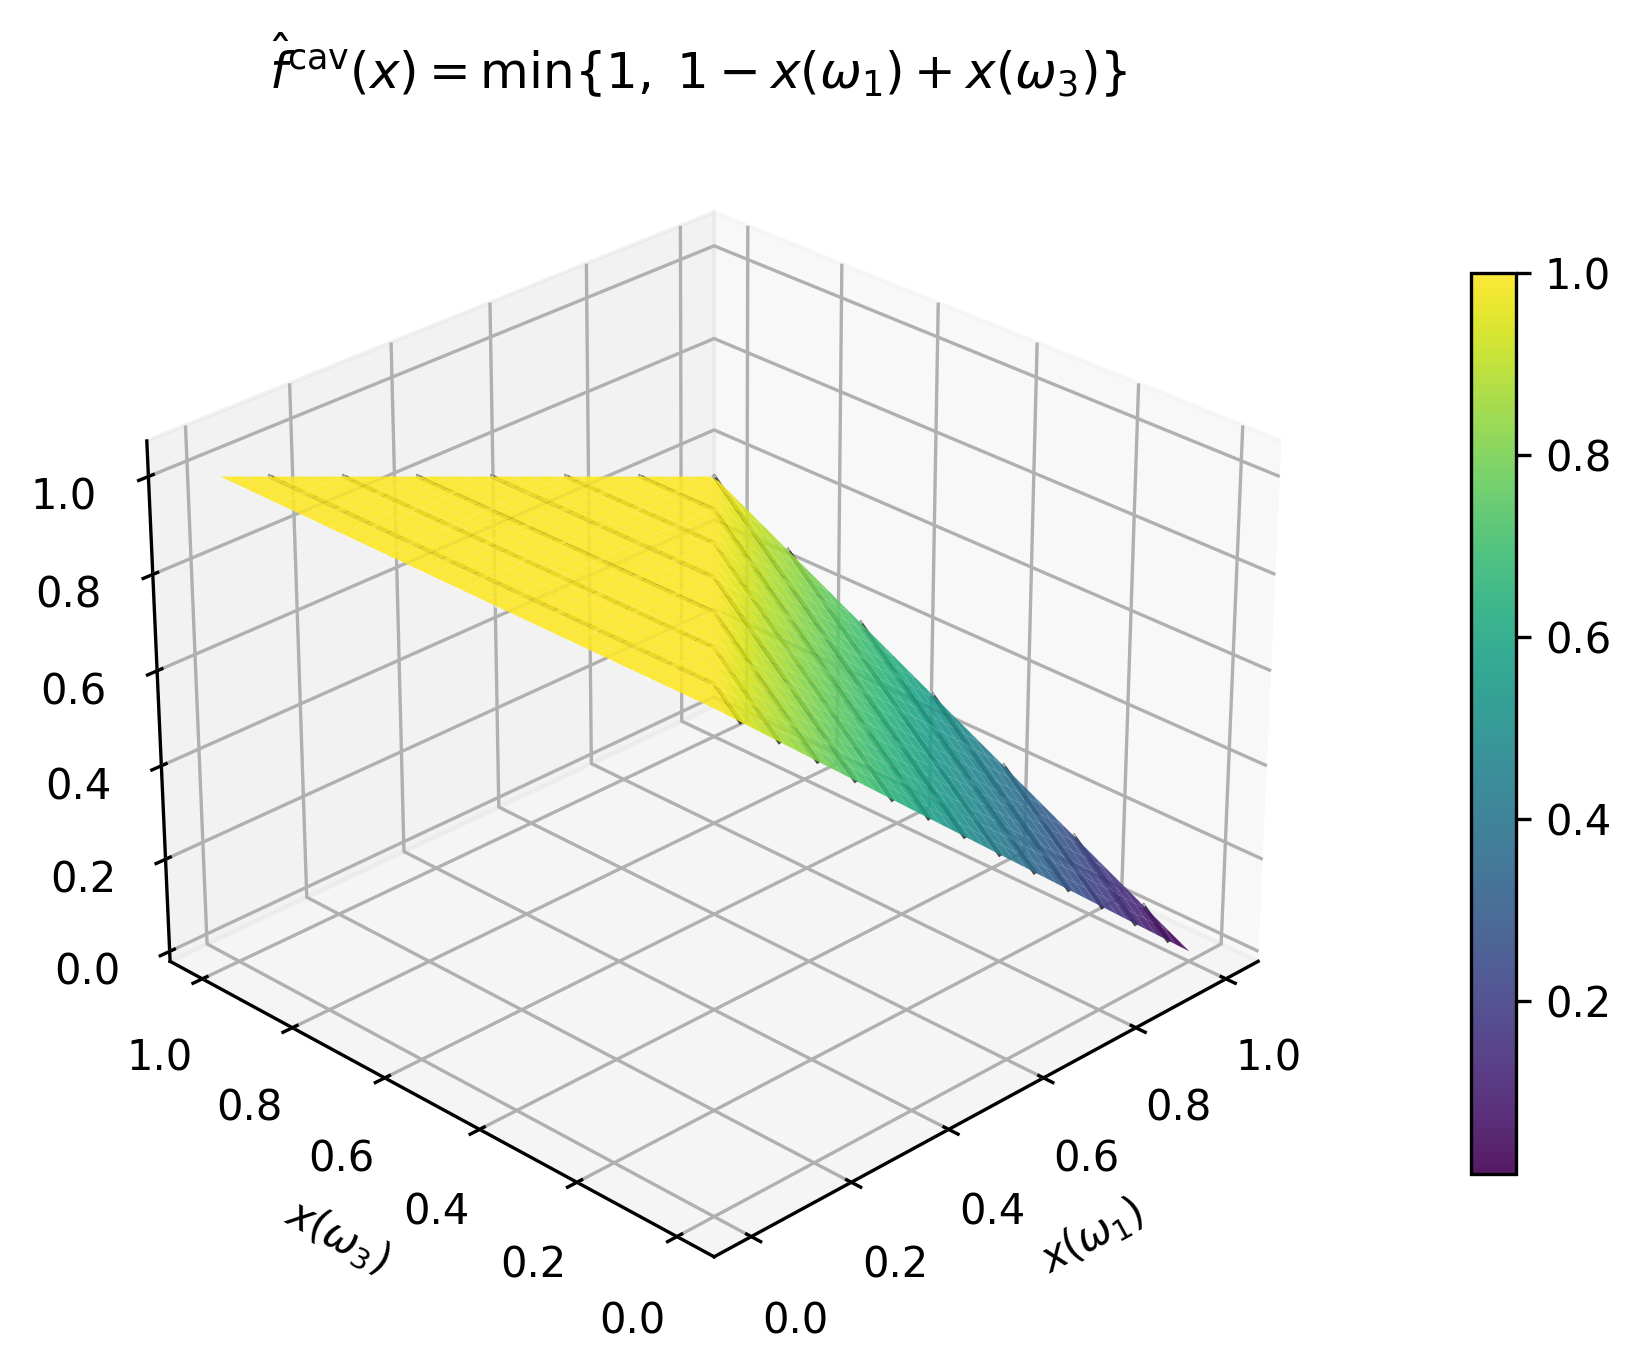
\includegraphics[scale=0.5]{hat_f_cav.png}
\begin{original}
\caption{Concave envelope $\widehat{f}^{\text{cav}}$}
\end{original}
\begin{translation}
\caption{凹包络$\widehat{f}^{\text{cav}}$}
\end{translation}
\label{fig1a}
\end{subfigure}
\quad \quad
\begin{subfigure}[b]{0.4\linewidth}
\centering
 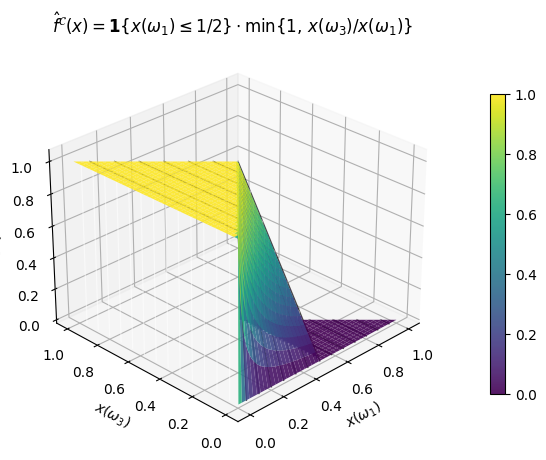
\includegraphics[scale=0.5]{hat_f_C_new.png}
\begin{original}
\caption{Privacy-preserving envelope $\widehat{f}^{\C}$}
\end{original}
\begin{translation}
\caption{隐私保护包络$\widehat{f}^{\C}$}
\end{translation}
\label{fig1b}
\end{subfigure}
\begin{original}
\caption{Comparison of envelopes}
\end{original}
\begin{translation}
\caption{包络的比较}
\end{translation}
\label{fig:persuasion}
\end{figure}

\paragraph{Sequential Sampling.}\hspace{-2mm}
\begin{original}
Another class of technologies that is automatically composition-closed is \textit{\textbf{dynamic sampling/stopping}} technologies. For example, \citet{brocas2007influence}, \citet{henry2019research}, \citet{morris2019wald}, and \citet{ball2021experimental} consider the classic Wald sampling model (\citealt{Wald}) adopted in information design settings. We describe a general setting in discrete time. Fix a finite state space $\Omega$. The belief process $(x_n)_{n \geq 0}$ taking values in $X = \Delta(\Omega)$ under any monitoring technology in the style of \citet{Wald} would evolve according to a time-homogeneous Markov martingale with some transition kernel $Q$.

A designer chooses a \textit{\textbf{randomized stopping time}} $\tau$ with
respect to the natural filtration of $(x_n)_{n \geq 0}$. The induced posterior distribution is the law of the stopped belief $x_\tau$. Every such $\tau$ generates a transition kernel $P^\tau$ on $X$ defined by
\[P^\tau(\,\cdot\, \mid x) = \P\big[x_\tau \in \,\cdot\, \mid x_0 = x\big]\,.\]
Let
\[\mathcal{P} := \Big\{P^\tau: \tau \text{ is a randomized stopping time for $(x_n)_{n\geq 0}$}\Big\}\,.\]
Then, it is evident that $\mathcal{P}$ is composition-closed and regular. Therefore, by \Cref{thm:main-compare}, there exists an order $\preceq_\C$ stronger than the Blackwell order on $\Delta(X)$ such that
\[\mu \preceq_\C \nu \iff \text{there exists a randomized stopping time $\tau$ s.t. $x_\tau  \sim \nu$ with $x_0 \sim \mu$\,.}\]
Therefore, any dynamic sampling/stopping problem is equivalent to a \textit{\textbf{reduced-form constrained information design}} for which \Cref{cor:envelope} and \Cref{prop:comparison} hold immediately---in particular, they admit envelope characterizations and satisfy structural properties just like in the unconstrained case studied in \citet{Kamenica2011}. Moreover, as \Cref{prop:comparison} shows, unless the constrained problem is value-eliminating,  the induced posterior distributions for any such problem must weakly Blackwell dominate the KG signal with a binary state, and cannot be strictly Blackwell dominated by the KG signal with any finite state.

What is the appropriate envelope here? By \Cref{cor:envelope}, the appropriate envelope $\widehat{f}$ is defined by $[-\Phi(\mathcal{P})]$-envelope of $f$. By definition, $g \in -\Phi(\mathcal{P})$ if and only if
\[\int g(y) P(\d y\mid x) \leq g(x) \text{ for all $x$ and all $P \in \mathcal{P}$}\,,\]
which is equivalent to
\[\int g(y) P^\tau(\d y\mid x) \leq g(x) \text{ for all $x$ and all randomized stopping times $\tau$}\,.\]
Since the Markov process is time-homogeneous, note that the above is equivalent to
\[\int g(y) Q(\d y\mid x) \leq g(x) \text{ for all $x$}\,,\]
where $Q$ is the transition kernel of the Markov process. In the language of optimal stopping theory, such a function is called a \textit{\textbf{superharmonic/excessive function}}. This provides a point of connection to the well-known \textit{\textbf{Dynkin's theorem}} (\citealt{dynkin1963optimal}) in optimal stopping. It is further generalized in  \citet{dayanik2003optimal} and states that the value function
\[V = \inf\Big\{g : g \text{ is excessive and } g \geq f \Big\}, \tag{\textbf{Dynkin}}\]
which our results immediately recover.

Combining \Cref{thm:main-compare} and the above observation about time-homogeneous Markov chains, we also immediately obtain:
\[\int g \d \mu \geq \int g \d \nu \text{ for all excessive $g$} \iff \text{$\exists$ $\tau$ s.t. $x_\tau  \sim \nu$ with $x_0 \sim \mu$\,,} \tag{\textbf{Rost}}\]
which is the well-known \textit{\textbf{Rost's theorem}} (\citealt{rost1971stopping}) in the theory of Skorokhod embeddings for Markov
processes. Rost's theorem is extremely useful for identifying the set of inducible posterior distributions from stopping a Markov chain, and has been applied in, e.g., \citet{morris2019wald}.

More generally, our results apply to the cases where (i) the Markov chain need not be time-homogeneous and (ii) the choice need not be an optimal stopping problem but a \textit{\textbf{control problem}}. Indeed, suppose in each period, the designer can choose from a feasible set of experiments (e.g., as studied in \citealt*{ni2023sequential}), which corresponds to a base set of Markov transition kernels. By the same logic as above, it follows immediately that the problem admits an envelope characterization, and the inducible posterior belief distributions can be characterized by an integral stochastic order.
\end{original}
\begin{translation}
另一类自动复合-封闭的技术是\textit{\textbf{动态抽样/停时}}技术。例如，\citet{brocas2007influence}、\citet{henry2019research}、\citet{morris2019wald}和\citet{ball2021experimental}考虑了在信息设计设定中采用的经典Wald抽样模型(\citealt{Wald})。我们描述一个离散时间的一般设定。信念过程$(x_n)_{n \geq 0}$在任何Wald式监测技术下的演化遵循时间齐次Markov鞅，具有某个转移核$Q$。

设计者关于$(x_n)_{n \geq 0}$的自然滤子选择一个\textit{\textbf{随机停时}}$\tau$。诱导的后验分布是停止信念$x_\tau$的分布。每个$\tau$生成$X$上的转移核$P^\tau$，定义为$P^\tau(\cdot \mid x) = \P[x_\tau \in \cdot \mid x_0 = x]$。令$\mathcal{P} := \{P^\tau: \tau \text{是}(x_n)_{n\geq 0}\text{的随机停时}\}$。则显然$\mathcal{P}$是复合-封闭和正则的。因此，由\Cref{thm:main-compare}，存在$\Delta(X)$上比Blackwell序更强的序$\preceq_\C$，使得$\mu \preceq_\C \nu \iff$存在随机停时$\tau$使得$x_\tau \sim \nu$且$x_0 \sim \mu$。

因此，任何动态抽样/停时问题等价于一个\textit{\textbf{简化型受约束信息设计}}，\Cref{cor:envelope}和\Cref{prop:comparison}对其直接成立——特别地，它们允许包络刻画并满足与\citet{Kamenica2011}中研究的无约束情形相同的结构性质。而且，如\Cref{prop:comparison}所示，除非受约束问题是值消除的，任何此类问题的诱导后验分布必须弱Blackwell支配二元状态的KG信号，且不能被任何有限状态的KG信号严格Blackwell支配。

这里合适的包络是什么？由\Cref{cor:envelope}，合适的包络$\widehat{f}$由$f$的$[-\Phi(\mathcal{P})]$-包络定义。$g \in -\Phi(\mathcal{P})$当且仅当对所有$x$和所有$P \in \mathcal{P}$有$\int g(y) P(\d y\mid x) \leq g(x)$，这等价于对所有$x$和所有随机停时$\tau$有$\int g(y) P^\tau(\d y\mid x) \leq g(x)$。由于Markov过程是时间齐次的，上式等价于对所有$x$有$\int g(y) Q(\d y\mid x) \leq g(x)$，其中$Q$是Markov过程的转移核。在最优停时理论的语言中，这样的函数称为\textit{\textbf{上调和/过分函数}}。这与最优停时中著名的\textit{\textbf{Dynkin定理}}(\citealt{dynkin1963optimal})建立了联系。该定理在\citet{dayanik2003optimal}中得到进一步推广，并陈述值函数$V = \inf\{g : g \text{是过分的且} g \geq f\}$，我们的结果立即恢复了这一点。

结合\Cref{thm:main-compare}和上述关于时间齐次Markov链的观察，我们也立即得到：$\int g \d \mu \geq \int g \d \nu$对所有过分函数$g$成立$\iff$存在$\tau$使得$x_\tau \sim \nu$且$x_0 \sim \mu$，这正是Markov过程的Skorokhod嵌入理论中著名的\textit{\textbf{Rost定理}}(\citealt{rost1971stopping})。Rost定理对于识别停止Markov链可诱导的后验分布集非常有用，并已应用于如\citet{morris2019wald}。

更一般地，我们的结果适用于(i) Markov链不必是时间齐次的，和(ii)选择不必是最优停时问题而可以是\textit{\textbf{控制问题}}的情形。确实，假设在每个时期，设计者可以从一集可行实验中选择（例如\citealt*{ni2023sequential}所研究的），这对应于一集基础Markov转移核。由与上述相同的逻辑，该问题立即允许包络刻画，且可诱导的后验信念分布可以由积分随机序刻画。
\end{translation}


\subsection{Which Updating Rules Admit Consistent Orders?}
\begin{original}
In \Cref{sec:Bayes-plausible}, we show that any Blackwell-consistent Bayes-plausible order on $\Delta(X)$ must be a strengthening of the Blackwell order. In particular, if the updating rule is fixed to be Bayes' rule, then the garbling order is necessary for there to be a Blackwell-consistent value-based order of information. Given this result, a natural question arises: are there other Blackwell-consistent value-based orders of information if the updating rule is allowed to be non-Bayesian? Without Bayesian updating, orders on $\Delta(X)$ need not be Bayes-plausible. We now apply \Cref{thm:main2} and \Cref{thm:main-compare} to characterize all possible updating rules that can admit a consistent order $\preceq$ on the set of posterior belief distributions (which need not be Bayes-plausible). It turns out that if we want to compare all experiments that are comparable by Blackwell's garbling criterion, then essentially the only possible updating rules are homeomorphic to Bayes' rule. To begin with, we first introduce a general framework for non-Bayesian updating.
\end{original}
\begin{translation}
在\Cref{sec:Bayes-plausible}中，我们证明$\Delta(X)$上的任何Blackwell-一致、贝叶斯-可信的序必须是Blackwell序的加强。特别地，如果更新规则固定为贝叶斯法则，那么garbling序对于存在Blackwell-一致的基于价值的信息序是必要的。给定这一结果，一个自然的问题出现了：如果允许更新规则是非贝叶斯的，是否存在其他Blackwell-一致的基于价值的信息序？在没有贝叶斯更新的情况下，$\Delta(X)$上的序不需要是贝叶斯-可信的。我们现在应用\Cref{thm:main2}和\Cref{thm:main-compare}来刻画所有可能在后验信念分布集（不必是贝叶斯-可信的）上允许一致序$\preceq$的更新规则。结果表明，如果我们想比较所有可通过Blackwell garbling准则比较的实验，那么本质上唯一可能的更新规则与贝叶斯法则同胚。首先，我们引入非贝叶斯更新的一般框架。
\end{translation}

\subsubsection{A General Framework for Non-Bayesian Updating}
\begin{original}
Let $\Omega$ be a finite set of states, and let $X:=\Delta(\Omega)$ be the set of beliefs over $\Omega$. \citet{cripps2018divisible} develops a general theory for \textit{\textbf{distorted updating rules}} which distort Bayesian posterior beliefs. A \textit{\textbf{(prior-dependent) systematic distortion}} of belief updates is a continuous function $d:X\times X \to X$, where $d(x, y) \in X$ denotes the distorted posterior belief when the prior is $x$ and the Bayesian posterior is $y$. For example, $d^{\mathrm{B}}(x, y) := y$ corresponds to the Bayesian updating rule without any distortion. We impose several regularity conditions on $d$: (i) $d$ is continuous; (ii) for any $x \in X^0:= \text{int } \Delta(\Omega), z \mapsto d(x,z)$ is injective on $X^0$; (iii) $d(x,x)=x$ for all $x \in X$.\footnote{These conditions, together with the convention that distorted updating rules are defined in terms of beliefs, correspond to Axioms 1-3 of \citet{cripps2018divisible}.} Let $\mathcal{D}$ be the set of such updating rules.

For any $d \in \mathcal{D}$, it is convenient to define
\[
\hat{d}(x_B,x_D,y):=d\left(x_D,\frac{x_D \oslash x_B \odot y}{\langle x_D \oslash x_B,y\rangle}\right)\,,
\]
for all $x_B,x_D,y \in X^0$, where $\oslash$ denotes the component-wise division of two vectors, and $\odot$ denotes the component-wise product of two vectors.\footnote{Since $d(x,y)$ is continuous, $\hat{d}$ can be extended continuously on $X \times X \times X$.} The function $\hat{d}(x_B,x_D,y)$ corresponds to the distorted belief where the distorted prior is $x_D$, and the Bayesian posterior is $y$, which is updated from a (potentially different) Bayesian prior $x_B \in X$. When the Bayesian prior is different from the distorted prior, the Bayesian posterior updated from the distorted prior is distinct from, but is determined by (up to a likelihood ratio), the Bayesian posterior updated from the Bayesian prior $x_B$. The second argument of the right-hand side makes this correction. It follows immediately from the definition that
\[
\hat{d}(x_B,x_B,y)=d(x_B,y)\,,\quad \quad \mbox{ and } \quad \quad \hat{d}(x_B,x_D,x_B)=x_D\,.
\]
That is, when the Bayesian prior $x$ is the same as the distorted prior, the distorted posterior given the Bayesian posterior is exactly given by $d(x,y)$. Moreover, when the Bayesian posterior equals the Bayesian prior $x_B$ (i.e., there is no Bayesian updating), the distorted posterior must be the same as the distorted prior $x_D$ (i.e., there is no distorted updating either).

While an updating rule $d \in \mathcal{D}$ describes only how beliefs will be updated (relative to Bayesian updating) from a single signal, it implies a natural description of how beliefs will be updated from multiple signals that arrive sequentially. To see this, for any updating rule $d \in \mathcal{D}$, let $d_{\mathrm{II}}:X \times X \times X \to X$ be defined by
\[
d_{\mathrm{II}}(x,z;y):=\hat{d}(y,d(x,y),z)=d\left(d(x,y),\frac{d(x,y)\oslash y \odot z}{\langle d(x,y)\oslash y,z \rangle}\right)\,,
\]
for all $x,y,z \in X^0$.\footnote{Since $d(x,y)$ is continuous, $d_{\mathrm{II}}$ can be extended continuously on $X \times X \times X$.} Under this definition, $d_{\mathrm{II}}(x,z;y)$ describes the terminal distorted posterior belief under a two-stage updating process, where one signal is drawn from a Blackwell experiment first, and then a second signal is drawn from another Blackwell experiment (which could potentially depend on the realization of the first signal). In this process, the prior is $x$, the first-stage Bayesian posterior belief is $y$ (and hence the first-stage interim distorted posterior belief is $d(x,y)$), and the second-stage Bayesian posterior belief is $z$. Clearly, if the updating rule is Bayesian, then sequentially updating must lead to the same outcome as if updating is done at once, and the terminal posterior belief would not depend on the realization of the interim belief $y$, conditional on $z$ itself. That is,
\[
d_{\mathrm{II}}^\mathrm{B}(x,z;y)=d^\mathrm{B}(x,z)=z\,,
\]
for all $x,y,z \in X^0$. We refer to updating rules that satisfy the same property as being \textit{\textbf{divisible}}. That is, we say that $d\in \mathcal{D}$ is divisible if $d(x,\cdot)$ is bijective for all $x \in X$, and
\[
d_{\mathrm{II}}(x,z;y)=d(x,z)\,,\tag{\textbf{Divisibility}}
\]
for all $x,y,z \in X^0$. Divisible updating rules have a compact characterization, due to \citet{cripps2018divisible}. Namely, for $d \in \mathcal{D}$, $d$ is divisible if and only if there exists a homeomorphism $F:X \to X$ such that
\[
d(x,y)=F^{-1}\left(\frac{F(x)\oslash x \odot y}{\langle F(x)\oslash x,y \rangle}\right)
\]
for all $x,y \in X^0$. When $F$ is the identity function, $d(x,y)$ is the Bayesian updating rule. In a sense, a divisible updating rule $d$ is \emph{essentially} Bayesian: it distorts the prior via a homeomorphism $F$, updates via Bayes' rule, and distorts the posterior back again via $F^{-1}$.
\end{original}
\begin{translation}
令$\Omega$为有限状态集，$X:=\Delta(\Omega)$为信念集。\citet{cripps2018divisible}发展了扭曲贝叶斯后验信念的\textit{\textbf{扭曲更新规则}}的一般理论。信念更新的\textit{\textbf{（先验依赖）系统性扭曲}}是一个连续函数$d:X\times X \to X$，其中$d(x, y) \in X$表示先验为$x$、贝叶斯后验为$y$时的扭曲后验信念。我们施加几个正则条件：(i) $d$连续；(ii) 对$x \in X^0$，$z \mapsto d(x,z)$在$X^0$上单射；(iii) $d(x,x)=x$对所有$x$成立。令$\mathcal{D}$为此类更新规则的集合。

对任意$d \in \mathcal{D}$，定义$\hat{d}(x_B,x_D,y):=d(x_D,\frac{x_D \oslash x_B \odot y}{\langle x_D \oslash x_B,y\rangle})$，其中$\oslash$表示逐分量除法，$\odot$表示逐分量乘法。$\hat{d}(x_B,x_D,y)$对应扭曲先验为$x_D$、贝叶斯后验为$y$的扭曲信念，该后验是从（可能不同的）贝叶斯先验$x_B$更新的。由定义立即有$\hat{d}(x_B,x_B,y)=d(x_B,y)$和$\hat{d}(x_B,x_D,x_B)=x_D$。

对任意更新规则$d \in \mathcal{D}$，定义$d_{\mathrm{II}}(x,z;y):=\hat{d}(y,d(x,y),z)$。$d_{\mathrm{II}}(x,z;y)$描述了两阶段更新过程下的终端扭曲后验信念。我们称满足$d_{\mathrm{II}}(x,z;y)=d(x,z)$的$d \in \mathcal{D}$是\textit{\textbf{可除}}的，如果$d(x,\cdot)$对所有$x$是双射。可除更新规则有简洁的刻画(\citet{cripps2018divisible})：$d$可除当且仅当存在同胚$F:X \to X$使得$d(x,y)=F^{-1}(\frac{F(x)\oslash x \odot y}{\langle F(x)\oslash x,y \rangle})$。当$F$是恒等函数时，$d(x,y)$即贝叶斯更新规则。在某种意义上，可除更新规则$d$\textit{本质上}是贝叶斯的：它通过同胚$F$扭曲先验，通过贝叶斯法则更新，再通过$F^{-1}$扭曲回来。
\end{translation}

\subsubsection{Consistent Comparisons under Non-Bayesian Updating}
\begin{original}
Let $\Pc_M$ be the set of all martingale kernels. For any $P \in \Pc_M$ and for any $x \in X$, we may interpret $P(\,\cdot\,\mid x)$ as the distribution over (Bayesian) posterior beliefs induced by a Blackwell experiment when the (Bayesian) prior is $x$. As noted before, the garbling order of Blackwell experiments can be represented by the order $\preceq^{\Pc_M}$ on $\Delta(X)$. Therefore, for there to be a Blackwell-consistent, value-based order on $\Delta(X)$, there has to be a class of problems under which the expected value under any $P(\,\cdot\,\mid x)$ is higher than the value at $x$, for all priors $x$. When $d \in \mathcal{D}$ is the Bayesian updating rule, by Blackwell's theorem, the class of problems are exactly decision problems (i.e., convex functions of posterior beliefs). When the updating rule $d \in \mathcal{D}$ is non-Bayesian, however, this is generally not the case.

To evaluate the value of information under a potentially non-Bayesian updating rule $d \in \mathcal{D}$, a natural perspective is to evaluate the expected value of a problem \emph{\textbf{paternalistically}}, as in \citet{whitmeyerforthcomingBlackwell}. From the paternalistic perspective, a decision is made under the distorted belief, whereas the expected value is computed using the Bayesian belief. Therefore, a problem would be described by a function $g:X \times X \to \R$, where $g(x_B,x_D)$ denotes the indirect value of a problem when the Bayesian belief, which is used to evaluate the expected value, is $x_B$, and when the distorted belief, which is used to determine the action, is $x_D$. For example, if the problem is a decision problem, with action set $A$ and payoff function $u$, then
\[
g(x_B,x_D)=\E_{\omega \sim x_B} [u(\omega,a^*(x_D))]
\]
is the indirect utility, where $a^*(x_D)$ is the optimal action under belief $x_D$. However, the problem need not be a decision problem; for example, it can be a non-Bayesian persuasion problem where $a^*(x_D)$ is the optimal action taken under the distorted belief $x_D$ and an objective $\tilde{u}$ different from $u$, with the payoff evaluated under the Bayesian posterior $x_B$ and the sender's objective $u$.

For the garbling order to have a Blackwell-consistent, value-based order, the relevant class of problems must be such that
\[
\int g(y, \hat{d}(x_B,x_D,y))P(\d y\mid x_B) \geq g(x_B,x_D)\,.
\]
That is, given any pair of Bayesian and distorted priors $(x_B,x_D)$, the expected paternalistic value of the problem with more information---given by $P(\,\cdot\,\mid x_B)$---must be higher than the value without any information. Let $\C^d \subseteq B(X \times X)$ be such functions.

Naturally, one might conjecture that the class of problems $\C^d$ dualizes the garbling-based comparison under the updating rule $d$. However, our next result shows that this is in general not the case. In fact, we show the garbling-based comparison admits a Blackwell-consistent value-based order if and only if $d$ is divisible. As a result, there is generally no instrumental-value-based representation of the garbling order once the updating rule is non-Bayesian, with the only exception being the case when the updating rule is divisible (i.e., being ``essentially'' Bayesian).

For any $(x_B,x_D)$, and for any $P \in \Pc_M$, let $Y$ be the random variable that follows $P(\,\cdot\,\mid x_B)$ and consider the distribution $Q$ of
\[
(Y,\hat{d}(x_B,x_D,Y))\,.
\]
If we interpret $x_B$ as the Bayesian prior, $x_D$ as a distorted prior, and $P(\,\cdot\,\mid x_B)$ as a Blackwell experiment (identified by the distribution of \emph{Bayesian} posterior beliefs), then $Q(\,\cdot\,\mid x_B,x_D)$ is the joint distribution of the Bayesian and $d$-distorted posterior beliefs under the same experiment. Let $\mathcal{Q}_0$ be the set of transition kernels on $X\times X$. Let
\[\mathcal{Q}^{d}_{(x_B, x_D)}:= \Big\{ \text{Law}(Y, \hat{d}(x_B,x_D,Y)): \text{ $Y$ is a random variable with $\E[Y]=x_B$ }\Big\}\,.\]
Let
\[
\cQ^d:=\Big\{Q \in \cQ_0:  Q(\,\cdot\,\mid x_B, x_D) \in \mathcal{Q}^{d}_{(x_B, x_D)} \text{ for all $x_B, x_D$} \Big\}
\]
denote the set of all distributions of posterior beliefs under the distorted updating rule $d$. Note that $\cQ^d$ is regular. Moreover, $\cQ^d$ defines a binary relation on $\Delta(X\times X)$, where $\mu \preceq^{\cQ^d} \nu$ if and only if $\nu=Q*\mu$ for some $Q \in \cQ^d$. By the definition of $\cQ^d$, the comparison given by $\preceq^{\cQ^d}$ encodes the garbling order of Blackwell experiments: for any $(x_B, x_D)$, by construction, $\delta_{(x_B, x_D)} \preceq^{\cQ^d} \nu$ if and only if $\nu$ is the joint  distribution of the Bayesian posterior and the distorted posterior under the updating rule $d$ for \textit{some} experiment $P$.

Our next result characterizes updating rules that admit consistent comparisons in the Blackwell sense by applying \Cref{thm:main2} to the space $X \times X$.
\end{original}
\begin{translation}
令$\Pc_M$为所有鞅核的集合。对任意$P \in \Pc_M$和$x \in X$，我们可以将$P(\,\cdot\,\mid x)$解释为当（贝叶斯）先验为$x$时Blackwell实验诱导的（贝叶斯）后验信念的分布。如前所述，Blackwell实验的garbling序可以由$\Delta(X)$上的序$\preceq^{\Pc_M}$表示。因此，要在$\Delta(X)$上存在Blackwell-一致的、基于价值的序，必须有一类问题，使得在任何$P(\,\cdot\,\mid x)$下的期望值高于在$x$处的值，且这对所有先验$x$成立。当$d \in \mathcal{D}$是贝叶斯更新规则时，由Blackwell定理，这类问题恰好是决策问题（即后验信念的凸函数）。然而，当更新规则$d \in \mathcal{D}$是非贝叶斯时，这通常不成立。

为在可能非贝叶斯的更新规则下评估信息价值，一种自然的视角是\textit{\textbf{家长式地}}评估一个问题的期望价值，如\citet{whitmeyerforthcomingBlackwell}所述。从家长式视角，决策是在扭曲信念下做出的，而期望值是用贝叶斯信念计算的。因此，一个问题将由函数$g:X \times X \to \R$描述，其中$g(x_B,x_D)$表示当贝叶斯信念为$x_B$、扭曲信念为$x_D$时问题的间接价值。

对garbling序具有Blackwell-一致、基于价值的序，相关的问题类必须满足：对任意贝叶斯和扭曲先验对$(x_B,x_D)$，
\[
\int g(y, \hat{d}(x_B,x_D,y))P(\d y\mid x_B) \geq g(x_B,x_D)\,.
\]
令$\C^d \subseteq B(X \times X)$为这样的函数。

人们可能自然猜测问题类$\C^d$在更新规则$d$下对偶化了基于garbling的比较。然而，我们的下一个结果表明这通常不是事实。实际上，我们证明基于garbling的比较允许Blackwell-一致的基于价值的序当且仅当$d$是可除的。因此，一旦更新规则是非贝叶斯的，garbling序通常没有基于工具价值的表示，唯一的例外是更新规则可除的情形（即``本质上''是贝叶斯的）。

对于任意$(x_B,x_D)$和$P \in \Pc_M$，令$Y$为服从$P(\,\cdot\,\mid x_B)$的随机变量，并考虑$(Y,\hat{d}(x_B,x_D,Y))$的分布$Q$。令$\mathcal{Q}^{d}_{(x_B, x_D)}:= \{\text{Law}(Y, \hat{d}(x_B,x_D,Y)): \text{$Y$为随机变量且$\E[Y]=x_B$}\}$。令$\cQ^d:=\{Q \in \cQ_0: Q(\,\cdot\,\mid x_B, x_D) \in \mathcal{Q}^{d}_{(x_B, x_D)} \text{对所有$x_B, x_D$}\}$为扭曲更新规则$d$下所有后验信念分布的集合。$\cQ^d$在$\Delta(X\times X)$上定义一个二元关系：$\mu \preceq^{\cQ^d} \nu$当且仅当对某个$Q \in \cQ^d$有$\nu=Q*\mu$。由$\cQ^d$的定义，$\preceq^{\cQ^d}$给出的比较编码了Blackwell实验的garbling序。

我们的下一个结果通过将\Cref{thm:main2}应用于空间$X \times X$来刻画允许Blackwell意义上一致比较的更新规则。
\end{translation}

\begin{prop}[Consistent Comparisons under Non-Bayesian Updating]\label{prop:divisible}
\begin{original}
The garbling-based comparison $\preceq^{\cQ^d}$ is a Blackwell-consistent order if and only if $d$ is divisible.
\end{original}
\begin{translation}
基于garbling的比较$\preceq^{\cQ^d}$是Blackwell-一致的序当且仅当$d$是可除的。
\end{translation}
\end{prop}

\begin{original}
Naturally, one might conjecture that the garbling comparison always has a dual representation in terms of its instrumental value just like in Blackwell's theorem under Bayes' rule. However, \Cref{prop:divisible} shows that this is \textit{false}. According to \Cref{prop:divisible}, when the updating rule $d$ is not divisible, there cannot be a value-based order that represents the garbling-based comparison $\preceq^{\cQ^d}$. In particular, there exist distributions of posterior beliefs $\mu,\nu \in \Delta(X \times X)$ such that $\nu=Q*\mu$ and the instrumental value for any problem $g \in \C^d$ is increased:
\[
\int g(x_B,x_D) \mu(\d x_B, \d x_D) \leq \int g(x_B,x_D) \nu (\d x_B, \d x_D)\,,
\]
and yet $Q \not\in \mathcal{Q}^d$, i.e., $Q$ cannot be represented via a garbling of an experiment under the updating rule $d$. Moreover, \Cref{prop:divisible} shows that when $d$ is divisible, $\preceq^{\cQ^d}$ is a Blackwell-consistent order---equivalent to the value-based order $\preceq_{\C^d}$---and thus Blackwell's theorem is preserved in this regard.

Given that the garbling-based comparison only has a dual representation under divisible updating rules, which are homeomorphic to Bayes' rule, one might naturally further conjecture that the class of problems $\C^d$, which dualizes the garbling order under a divisible updating rule $d$, is the class of decision problems just like in Blackwell's theorem. However, this is again \textit{false}. Indeed, by the characterization of \citet{whitmeyerforthcomingBlackwell}, any non-Bayesian divisible updating rule is \textit{not} Blackwell-monotone, and hence there exists a decision problem under which a more informative experiment according to the garbling order leads to a lower paternalistic payoff. Nonetheless, by \Cref{prop:divisible}, a divisible updating rule is Blackwell-consistent, and therefore such a decision problem cannot appear in the class of problems that dualizes the garbling order under the divisible updating rule. In other words, combining \citet{whitmeyerforthcomingBlackwell} and \Cref{prop:divisible}, we then know that the class of problems that dualizes the garbling order under a divisible, non-Bayesian updating rule is \textit{not} the class of all decision problems. It necessarily excludes \textit{some} decision problem and may include \textit{some} persuasion problem or costly information acquisition problem---and yet, it dualizes the garbling order for a divisible updating rule according to \Cref{prop:divisible}.
\end{original}
\begin{translation}
人们可能自然猜测garbling比较总是有关于其工具价值的双重表示，就像贝叶斯法则下的Blackwell定理一样。然而，\Cref{prop:divisible}表明这是\textit{错误的}。根据\Cref{prop:divisible}，当更新规则$d$不可除时，不可能存在表示基于garbling的比较$\preceq^{\cQ^d}$的、基于价值的序。特别地，存在后验信念分布$\mu,\nu \in \Delta(X \times X)$使得对任何问题$g \in \C^d$有$\nu=Q*\mu$且工具价值增加了，但$Q \not\in \mathcal{Q}^d$，即$Q$不能通过更新规则$d$下的实验garbling表示。而且，\Cref{prop:divisible}表明当$d$可除时，$\preceq^{\cQ^d}$是Blackwell-一致的序——等价于基于价值的序$\preceq_{\C^d}$——因此在这方面Blackwell定理得以保持。

鉴于基于garbling的比较只在可除更新规则下有双重表示，而可除更新规则与贝叶斯法则同胚，人们可能自然进一步猜测，在可除更新规则$d$下对偶化garbling序的问题类$\C^d$就是决策问题类，就像Blackwell定理中一样。然而，这同样是\textit{错误的}。事实上，根据\citet{whitmeyerforthcomingBlackwell}的刻画，任何非贝叶斯可除更新规则\textit{不是}Blackwell-单调的，因此存在一个决策问题，在该问题下按照garbling序更具信息量的实验导致更低的家长式收益。然而，由\Cref{prop:divisible}，可除更新规则是Blackwell-一致的，因此这样的决策问题不能出现在对偶化该可除更新规则下garbling序的问题类中。换句话说，结合\citet{whitmeyerforthcomingBlackwell}和\Cref{prop:divisible}，我们知道在可除、非贝叶斯更新规则下对偶化garbling序的问题类\textit{不是}所有决策问题的类。它必然排除\textit{某些}决策问题，而可能包括\textit{某些}说服问题或成本信息获取问题——然而，根据\Cref{prop:divisible}，它确实对偶化了该可除更新规则下的garbling序。
\end{translation}

\subsubsection{Dynamic Values and Optimization under Non-Bayesian Updating}
\begin{original}
Similar to \Cref{sec:Bayes-plausible}, by virtue of \Cref{thm:main}, our results have immediate implications for optimization problems. In particular, we now show how \Cref{prop:divisible} yields new insights into information design problems with non-Bayesian updating (see, e.g., \citealt{alonso2016bayesian,de2022non,azrieli2025sequential,kobayashi2025dynamic}).

In information design problems with a non-Bayesian receiver, the sender's problem is equivalent to choosing a martingale $P \in \Pc_M$ to maximize
\[
\int f(y,\hat{d}(x_B,x_D,y))P(\d y\mid x_B)
\]
for a fixed (potentially heterogeneous) prior $(x_B,x_D)$, where $f:X \times X \to \R$ is the (Bayesian) sender's indirect utility that depends on the sender's Bayesian belief and the receiver's $d$-distorted belief. The optimal value of such a persuasion problem, as shown by \citet{alonso2016bayesian} and \citet{de2022non}, can be geometrically characterized by the concave envelope of the function $y \mapsto f(y,\hat{d}(x_B,x_D,y))$ evaluated at the prior $(x_B,x_D)$. However, a crucial implication of \Cref{prop:divisible} is that, when the updating rule is not divisible, such envelopes do not correspond to the functions that dualize the garbling order. In particular, the envelope is prior-dependent. Indeed, by \Cref{thm:main-compare}, the sender may improve their payoff by sending signals \textit{\textbf{sequentially}}, and static/one-shot persuasion would not be optimal in general.

To formalize this, for any $d \in \mathcal{D}$ and $x_B,x_D \in X$, consider the problem
\begin{equation*}
\sup_{Q \in \cQ^{d} \otimes \cQ^d} \int f(y_B,y_D) Q(\d y_B, \d y_D \mid x_B,x_D)\,. \eqtag[-2.5em][0.8\baselineskip]{\textbf{Dynamic}}{eq:two-stage}
\end{equation*}
In particular, \weqref{\textbf{Dynamic}}{eq:two-stage} could be interpreted as a dynamic information design problem with a non-Bayesian receiver, potentially with a different prior than the Bayesian sender, in which case $f(y_B,y_D)=v(y_B,a^*(y_D))$ is the sender's payoff as a function of the sender's own Bayesian prior and the receiver's optimal action taken in the second period given the distorted posterior belief. When information is costless and the sender only cares about the receiver's action, $v(y_B, a) = \E_{\omega \sim x_B} [u(\omega, a)]$ would be affine in $y_B$; however, when information is costly to the sender as in \citet{gentzkow2014costly}, or when the sender cares about the information intrinsically for their own action, $v(y_B, a)$ would not be affine in $y_B$. More generally, our formulation captures all information design problems in which the sender's payoff depends on the Bayesian and distorted posterior beliefs.

When $d$ is the Bayesian updating rule, in our setting, it is well-known that dynamic information design does not have any additional value compared to one-shot information design. Without Bayesian updating, there could be a benefit for dynamic information design. We say that $d \in \mathcal{D}$ admits \textit{\textbf{no dynamic value}} if for all $x_B,x_D \in X$, and for any upper semicontinuous $f: X\times X \to \R$,
\[
\sup_{Q \in \cQ^{d} \otimes \cQ^d} \int f(y_B,y_D) Q(\d y_B, \d y_D\mid x_B,x_D)=\sup_{Q \in \cQ^d} \int f(y_B,y_D) Q(\d y_B, \d y_D\mid x_B, x_D)\,.
\]
\end{original}
\begin{translation}
与\Cref{sec:Bayes-plausible}类似，凭借\Cref{thm:main}，我们的结果对优化问题有直接的含义。特别地，我们现在展示\Cref{prop:divisible}如何为非贝叶斯更新下的信息设计问题（见\citealt{alonso2016bayesian,de2022non,azrieli2025sequential,kobayashi2025dynamic}）提供新洞见。

在具有非贝叶斯接收者的信息设计问题中，发送者的问题等价于选择鞅$P \in \Pc_M$以最大化$\int f(y,\hat{d}(x_B,x_D,y))P(\d y\mid x_B)$，其中$f:X \times X \to \R$是（贝叶斯）发送者的间接效用，依赖于发送者的贝叶斯信念和接收者的$d$-扭曲信念。如\citet{alonso2016bayesian}和\citet{de2022non}所示，这种说服问题的最优值可以通过函数$y \mapsto f(y,\hat{d}(x_B,x_D,y))$的凹包络在$(x_B,x_D)$处取值来几何刻画。然而，\Cref{prop:divisible}的一个关键含义是，当更新规则不可除时，这样的包络不对应于对偶化garbling序的函数。特别地，包络是先验依赖的。确实，由\Cref{thm:main-compare}，发送者可以通过\textit{\textbf{序贯地}}发送信号来提高收益，而静态/一次性说服在一般情况下不是最优的。

为形式化这一点，对任意$d \in \mathcal{D}$和$x_B,x_D \in X$，考虑问题
\begin{equation*}
\sup_{Q \in \cQ^{d} \otimes \cQ^d} \int f(y_B,y_D) Q(\d y_B, \d y_D \mid x_B,x_D)\,. \eqtag[-2.5em][0.8\baselineskip]{\textbf{动态}}{eq:two-stage}
\end{equation*}
特别地，\weqref{\textbf{Dynamic}}{eq:two-stage}可被解释为具有非贝叶斯接收者的动态信息设计问题，其中$f(y_B,y_D)=v(y_B,a^*(y_D))$。当信息无成本且发送者只关心接收者的行动时，$v(y_B, a)$在$y_B$中是仿射的；然而，当信息对发送者有成本时（如\citet{gentzkow2014costly}），或当发送者出于自身行动本质上关心信息时，$v(y_B, a)$在$y_B$中不是仿射的。更一般地，我们的设定捕获了发送者收益依赖于贝叶斯和扭曲后验信念的所有信息设计问题。

当$d$是贝叶斯更新规则时，已知动态信息设计与一次性信息设计相比没有任何额外的价值。没有贝叶斯更新时，动态信息设计可能有益。我们称$d \in \mathcal{D}$允许\textit{\textbf{无动态价值}}，如果对所有$x_B,x_D \in X$和任意上半连续$f: X\times X \to \R$，有$\sup_{Q \in \cQ^{d} \otimes \cQ^d} \int f \d Q = \sup_{Q \in \cQ^d} \int f \d Q$。
\end{translation}

\begin{cor}\label{cor:dynamic}
\begin{original}
An updating rule $d \in \mathcal{D}$ admits no dynamic value if and only if $d$ is divisible.
\end{original}
\begin{translation}
更新规则$d \in \mathcal{D}$允许无动态价值当且仅当$d$是可除的。
\end{translation}
\end{cor}

\begin{original}
The sufficiency part of \Cref{cor:dynamic} immediately reproduces the result of \citet{kobayashi2025dynamic}, and extends it to \emph{all} information design problems, including persuasion problems where the sender's payoff is state-dependent. Moreover, \Cref{cor:dynamic} also answers the question raised in \citet{azrieli2025sequential} and \citet{kobayashi2025dynamic} by proving the converse---whenever the updating rule is not divisible, there exists \textit{some} information design problem where the sender can strictly benefit from sending signals sequentially.
\end{original}
\begin{translation}
\Cref{cor:dynamic}的充分性部分直接复现了\citet{kobayashi2025dynamic}的结果，并将其扩展到\textit{所有}信息设计问题，包括发送者收益依赖于状态的说服问题。此外，\Cref{cor:dynamic}还通过证明逆命题回答了\citet{azrieli2025sequential}和\citet{kobayashi2025dynamic}中提出的问题——每当更新规则不可除时，存在\textit{某种}信息设计问题，其中发送者可以从序贯发送信号中严格获益。
\end{translation}

\section{Nested Optimization and Stackelberg Principals}\label{sec:stackelberg}

\begin{original}
We now describe in more detail the nested optimization problem and give a few examples that arise in information design, decision theory, and mechanism design.
\end{original}
\begin{translation}
我们现在更详细地描述嵌套优化问题，并给出在信息设计、决策理论和机制设计中出现的几个例子。
\end{translation}

\subsection{General Framework}
\begin{original}
There are two principals $A$ and $B$. Principal $A$ is the \textit{\textbf{Stackelberg leader}} who chooses a measure $\mu \in M \subseteq \Delta(X)$, where $M$ is a compact convex set. Principal $B$ is the \textit{\textbf{Stackelberg follower}} who chooses a measure $\nu \preceq_{\C} \mu$ after principal $A$ has moved, where $\preceq_\C$ is an integral stochastic order. Principal $B$ solves a stochastic optimization problem as in \Cref{sec:abstract}:
\[\max_{\nu \preceq_\C \mu}\int f(x) \nu(\d x)\,.\]
Recall that $X^\star_f(\mu)$ is the solution correspondence of this problem.

Principal $A$ solves a nested optimization problem anticipating the effect on the follower. We assume that principal $B$ breaks ties in favor of principal $A$ so that principal $A$'s problem always has a solution. Formally, principal $A$ cares about the pair of measures $(\mu, \nu)$ selected at the end of the game, and thus solves the nested optimization as in \Cref{sec:abstract}:
\begin{equation*}
\text{ } \qquad \max_{(\mu,\nu) \in G^M_f} W(\mu,\nu)\,,
\end{equation*}
where $W$ is some continuous quasi-convex functional describing the principal's preferences and $G^M_f$ is the graph of the solution correspondence of principal $B$, i.e.,
\[G^M_f = \big\{(\mu,\nu): \mu \in M\,, \nu \in X^\star_f(\mu)\big\} \subseteq \Delta(X) \times \Delta(X)\,.\]
Formally, our solution concept is \textit{\textbf{leader-optimal subgame perfect equilibria}} (also known as strong Stackelberg equilibria).

By \Cref{cor:nested-optimization}, which is an immediate consequence of \Cref{thm:main}, we know that whenever $\C$ satisfies the min-closure property, there must exist an equilibrium in which (i) principal $A$ selects $\mu \in \Ext(M)$ and then (ii) principal $B$ selects $\nu \in \Ext(X^{\star}_f(\mu))$.

Moreover, in the case where $W(\mu, \nu)$ is a linear functional and hence can be written as $\int w_A(x) \mu(\d x) + \int w_B(x) \nu(\d x)$, we can explicitly construct all equilibria by invoking \Cref{thm:main}. To see this, let
\[w_B^\star(x):= \max_{\eta \in X^\star_f(\delta_x)} \int w_B(y) \eta(\d y) \quad \text{ and }\quad \mathcal{P}^\star_B(x):= \argmax_{\eta \in X^\star_f(\delta_x)} \int w_B(y) \eta(\d y)\,.\]
Then, we immediately have:
\end{original}
\begin{translation}
有两个委托人$A$和$B$。委托人$A$是\textit{\textbf{Stackelberg领导者}}，选择一个测度$\mu \in M \subseteq \Delta(X)$，其中$M$是紧凸集。委托人$B$是\textit{\textbf{Stackelberg追随者}}，在委托人$A$行动后选择一个测度$\nu \preceq_{\C} \mu$，其中$\preceq_\C$是积分随机序。委托人$B$解一个如\Cref{sec:abstract}中的随机优化问题：$\max_{\nu \preceq_\C \mu}\int f(x) \nu(\d x)$。回忆$X^\star_f(\mu)$是该问题的解对应。

委托人$A$预期对追随者的影响，解一个嵌套优化问题。我们假设委托人$B$在无差异时偏向委托人$A$，使得委托人$A$的问题总有解。形式上，委托人$A$关心博弈结束时选择的测度对$(\mu, \nu)$，因此如\Cref{sec:abstract}中解嵌套优化：$\max_{(\mu,\nu) \in G^M_f} W(\mu,\nu)$，其中$W$是描述委托人偏好的连续拟凸泛函，$G^M_f$是委托人$B$的解对应图。形式上，我们的解概念是\textit{\textbf{领导者最优子博弈完美均衡}}（也称强Stackelberg均衡）。

由\Cref{cor:nested-optimization}（\Cref{thm:main}的直接推论），我们知道每当$\C$满足最小-封闭性质时，必然存在一个均衡，其中(i) 委托人$A$选择$\mu \in \Ext(M)$，然后(ii) 委托人$B$选择$\nu \in \Ext(X^{\star}_f(\mu))$。

此外，在$W(\mu, \nu)$是线性泛函从而可写为$\int w_A(x) \mu(\d x) + \int w_B(x) \nu(\d x)$的情形中，我们可以借助\Cref{thm:main}显式构造所有均衡。为此，令$w_B^\star(x):= \max_{\eta \in X^\star_f(\delta_x)} \int w_B(y) \eta(\d y)$和$\mathcal{P}^\star_B(x):= \argmax_{\eta \in X^\star_f(\delta_x)} \int w_B(y) \eta(\d y)$。则我们立即得到：
\end{translation}

\begin{cor}\label{cor:modified}
\begin{original}
Suppose $\C$ is min-closed. The leader value of any leader-optimal equilibrium is
\[\max_{\mu \in M} \int (w_A(x) + w^\star_B(x)) \mu(\d x)\,.   \eqtag[-2.5em]{\textbf{Modified Objective}}{eq:modified}\]
Moreover, $(\mu, \nu)$ is a leader-optimal equilibrium if and only if
\begin{itemize}
    \item[(i)] $\mu$ maximizes \weqref{\textbf{Modified Objective}}{eq:modified} ;
    \item[(ii)] $\nu = P * \mu$ for some $P$ such that $P(\,\cdot\,\mid x) \in \mathcal{P}^\star_B(x)$ for $\mu$-a.e. $x$.
\end{itemize}
\end{original}
\begin{translation}
假设$\C$是最小-封闭的。任何领导者最优均衡的领导者值为
\[\max_{\mu \in M} \int (w_A(x) + w^\star_B(x)) \mu(\d x)\,.   \eqtag[-2.5em]{\textbf{修正目标}}{eq:modified}\]
此外，$(\mu, \nu)$是领导者最优均衡当且仅当
\begin{itemize}
    \item[(i)] $\mu$最大化\weqref{\textbf{Modified Objective}}{eq:modified}；
    \item[(ii)] $\nu = P * \mu$对某个$P$成立，使得$P(\,\cdot\,\mid x) \in \mathcal{P}^\star_B(x)$对$\mu$-a.e. $x$成立。
\end{itemize}
\end{translation}
\end{cor}

\begin{original}
Moreover, if the convex set $M$ for principal $A$ is also described by a stochastic orbit of the form $\{\mu: \mu \preceq_{\C_A} \gamma\}$ where $\C_A$ is min-closed and $\gamma$ is an exogenous measure, then by \Cref{thm:main} again, the leader value is simply given by
\[\int \overline{w^\star}(x) \gamma(\d x)\]
where $w^\star = w_A + w^\star_B$ and the envelope above is taken with respect to the set $\C_A$ and any leader-optimal strategy $\mu$ can only be supported on $\{x: \overline{w^\star}(x) = w^\star(x)\}$. While the above setup is described via the leader-optimal selection, any selection rule is compatible with our approach with the only difference being that the definition of $w^\star_B$ and $\Pc^\star_B$  will be modified accordingly.
\end{original}
\begin{translation}
此外，如果委托人$A$的凸集$M$也由形式为$\{\mu: \mu \preceq_{\C_A} \gamma\}$的随机轨道描述，其中$\C_A$是最小-封闭的，$\gamma$是外生测度，那么由\Cref{thm:main}再次，领导者值简单地由$\int \overline{w^\star}(x) \gamma(\d x)$给出，其中$w^\star = w_A + w^\star_B$，上述包络是对集合$\C_A$取的，且任何领导者最优策略$\mu$只能支撑在$\{x: \overline{w^\star}(x) = w^\star(x)\}$上。虽然上述设定是通过领导者最优选择描述的，但任何选择规则都与我们的方法兼容，唯一的区别是$w^\star_B$和$\Pc^\star_B$的定义将相应修正。
\end{translation}

\subsection{Economic Applications}

\begin{original}
We now describe a series of examples where our general results apply.
\end{original}
\begin{translation}
我们现在描述我们的通用结果适用的一系列例子。
\end{translation}

\paragraph{Sequential Persuasion.}\hspace{-2mm}
\begin{original}
Consider the following setting adapted from \citet{LiNorman2021SequentialPersuasion}. There is a finite state space $\Omega$. There are two senders. Sender $A$ designs a Blackwell experiment first, and then after observing $A$'s choice, sender $B$ designs an additional Blackwell experiment that can depend on the signal realization of $A$'s experiment. The receiver observes both experiments and both realized signals and takes an action from a finite set. This model corresponds to the case where $X = \Delta(\Omega)$, $\preceq_\C$ is the concave order, and $M = \{\mu: \mu \preceq_\C \delta_{x_0}\}$ where $x_0$ is the common prior about the state. As an immediate consequence of our results (\Cref{cor:modified}), there always exists a \textit{\textbf{sequential extremal equilibrium}} in which every sender $i$ selects an extreme point $\mu_i$ of $\text{MPS}(\mu_{i-1})$ where $\mu_{i-1}$ is the belief distribution selected by the previous sender. In particular, in this equilibrium, along any history, \textit{every} sender sends a signal with support size at most $|\Omega|$ \textit{as if} the subsequent senders do not exist, unlike in the \textit{\textbf{one-shot equilibria}} characterized in \citet{LiNorman2021SequentialPersuasion} in which the first sender splits beliefs in the set of ``stable beliefs'' and the subsequent senders all stay silent (also known as \textit{\textbf{silent equilibria}} in \citealt{wu2023sequential}).
\end{original}
\begin{translation}
考虑\citet{LiNorman2021SequentialPersuasion}的以下设定。有限状态空间$\Omega$，有两个发送者。发送者$A$首先设计一个Blackwell实验，然后观察到$A$的选择后，发送者$B$设计一个额外的Blackwell实验（可依赖于$A$实验的信号实现）。接收者观察两个实验和两个实现的信号，从有限集中选择行动。该模型对应$X = \Delta(\Omega)$，$\preceq_\C$是凹序，$M = \{\mu: \mu \preceq_\C \delta_{x_0}\}$。作为我们结果(\Cref{cor:modified})的直接推论，总是存在一个\textit{\textbf{序贯极端均衡}}，其中每个发送者$i$选择$\text{MPS}(\mu_{i-1})$的极端点$\mu_i$。特别地，在该均衡中，沿任何历史，\textit{每个}发送者都发送支撑大小至多$|\Omega|$的信号，\textit{仿佛}后续发送者不存在，这与\citet{LiNorman2021SequentialPersuasion}中刻画的一\textit{\textbf{次性均衡}}不同，后者中第一个发送者在``稳定信念''集中分裂信念，后续发送者都保持沉默（\citealt{wu2023sequential}中也称为\textit{\textbf{沉默均衡}}）。
\end{translation}

\paragraph{Robust Persuasion.}\hspace{-2mm}
\begin{original}
Consider the following setting adapted from \citet{DworczakPavan2022RobustPersuasion}. Again, there is a finite state space $\Omega$ and two senders who move sequentially just like in sequential persuasion. However, the second sender, who chooses an additional experiment after observing the realized signal of the first sender, is the \textit{\textbf{adversarial nature}} whose objective is to minimize the payoff of the first sender. Because the second mover has completely opposite preferences to the first mover, the leader-optimal selection rule here has no bite: The set of all SPEs---which correspond to the \textit{\textbf{worst-case optimal signals}} in \citet{DworczakPavan2022RobustPersuasion}---is exactly the leader-optimal SPEs, characterized by \Cref{cor:modified}. In particular, the modified objective in \Cref{cor:modified} is given by the \textit{\textbf{lower convex envelope}} of the initial sender's indirect utility function $V$ (assuming the receiver has a unique best response at any posterior belief). Since the initial sender's problem has the constraint set $M = \{\mu: \mu \preceq_\C \delta_{x_0}\}$ also given by a stochastic orbit, the leader value of this game must be given by the concavification of the lower convex envelope $V_{\text{lcx}}$, evaluated at the prior $x_0$, which is the \textit{\textbf{full information payoff}} where the initial sender just releases all information. Moreover, a posterior distribution $\mu \in \Delta(X)$ is induced by a worst-case optimal signal if and only if \[\supp(\mu) \subseteq \Big\{x:  V_{\text{lcx}}(x) = \widehat{V_{\text{lcx}}}^{\text{cav}}(x)  = V_{\text{full}}(x)\Big\} =: Y\,,\]
where $V_{\text{full}}(x)$ is the affine function describing the payoff of the initial sender given prior $x$ and release of full information. \citet{DworczakPavan2022RobustPersuasion} consider a refinement of worst-case optimal signals, the \textit{\textbf{robust solutions}}, which maximize the initial sender's indirect utility function among the worst-case optimal signals and therefore corresponds to solving a standard persuasion problem with a support restriction that $\supp(\mu) \subseteq Y$. For any non-affine $V_{\text{lcx}}$, note that any interior belief $x \in \text{int}(\Delta(\Omega))$ cannot be in $Y$ because then by construction it implies that $V_{\text{lcx}}$ is an affine function. Therefore, as observed in \citet{DworczakPavan2022RobustPersuasion}, any worst-case optimal signal must induce \textit{\textbf{separation}} of states where the support of any worst-case optimal $\mu$ must rule out some states. In fact, for any subset $B \subset \Omega$, the same argument implies that for any $x \in \text{int}(\Delta(B))$ to be in $Y$,  $V_{\text{lcx}} \mid_{\Delta(B)}$ must be an affine function coinciding with $V_{\text{full}} \mid_{\Delta(B)}$ which happens if and only if $V\mid_{\Delta(B)} \geq V_{\text{full}} \mid_{\Delta(B)}$; conversely, if $V_{\text{lcx}} \mid_{\Delta(B)}$ coincides with $V_{\text{full}} \mid_{\Delta(B)}$, then any $x \in \Delta(B)$ is in $Y$. Together, these characterize a set $\mathcal{F}$ of subsets $B \subset \Omega$ such that $x \in Y$ if and only if $\supp(x) \in \mathcal{F}$, which is the main separation theorem (Theorem 1) of \citet{DworczakPavan2022RobustPersuasion}.
\end{original}
\begin{translation}
考虑\citet{DworczakPavan2022RobustPersuasion}的以下设定。同样有有限状态空间$\Omega$和两个序贯行动的发送者。但第二个发送者是对抗性自然，其目标是最小化第一个发送者的收益。由于第二行动者与第一行动者有完全相反的偏好，此处领导者最优选择规则没有约束力：所有SPE的集合——对应\citet{DworczakPavan2022RobustPersuasion}中的\textit{\textbf{最坏情形最优信号}}——恰好是领导者最优SPE，由\Cref{cor:modified}刻画。特别地，\Cref{cor:modified}中的修正目标由初始发送者间接效用函数$V$的\textit{\textbf{下凸包络}}给出。由于初始发送者的问题具有同样由随机轨道给出的约束集$M = \{\mu: \mu \preceq_\C \delta_{x_0}\}$，该博弈的领导者值必须由下凸包络$V_{\text{lcx}}$在$x_0$处取值的凹化给出，即初始发送者释放全部信息的\textit{\textbf{完全信息收益}}。此外，后验分布$\mu$由最坏情形最优信号诱导当且仅当$\supp(\mu) \subseteq \{x: V_{\text{lcx}}(x) = \widehat{V_{\text{lcx}}}^{\text{cav}}(x) = V_{\text{full}}(x)\} =: Y$。\citet{DworczakPavan2022RobustPersuasion}考虑了最坏情形最优信号的一个精炼，\textit{\textbf{稳健解}}，在最坏情形最优信号中最大化初始发送者的间接效用函数，因此对应求解一个带支撑限制$\supp(\mu) \subseteq Y$的标准说服问题。对任何非仿射的$V_{\text{lcx}}$，注意任何内部信念$x \in \text{int}(\Delta(\Omega))$不能在$Y$中，因为这构造性地意味着$V_{\text{lcx}}$是仿射函数。因此，任何最坏情形最优信号必须诱导状态的\textit{\textbf{分离}}。这些一起刻画了子集$B \subset \Omega$的集合$\mathcal{F}$使得$x \in Y$当且仅当$\supp(x) \in \mathcal{F}$，这正是\citet{DworczakPavan2022RobustPersuasion}的主要分离定理（定理1）。
\end{translation}

\paragraph{Objective Ambiguity Aversion.}\hspace{-2mm}
\begin{original}
Consider the following setting adapted from \citet{olszewski2007preferences} and \citet{Ahn2008AmbiguityWithoutStateSpace} who study \textit{\textbf{objective ambiguity aversion}} of a decision maker by interpreting ambiguity as a menu of lotteries. The set of outcomes $X$ is a compact set in $\R^n$. A \textit{\textbf{lottery}} $\mu \in \Delta(X)$ specifies a distribution over outcomes. A \textit{\textbf{menu}} $A$ is a set of lotteries. \citet{olszewski2007preferences} and \citet{Ahn2008AmbiguityWithoutStateSpace} characterize preferences over menus of lotteries and formalize the notion of objective ambiguity aversion. Specifically, under a standard set of axioms, \citet{olszewski2007preferences}  shows that the representation of objective ambiguity-averse preference takes the following form:
\[
\mathcal{V}(A) := \alpha \cdot \max_{\mu \in A} \int u(x) \mu(\d x) + (1 - \alpha) \cdot \min_{\mu \in A} \int u(x) \mu(\d x)\,,
\]
for some function $u$, and some constant $\alpha \in [0, 1]$. In other words, the objective ambiguity-aversion representation takes the Hurwicz max-min form: the decision maker evaluates menus by computing the ``best-case'' payoff and the ``worst-case'' expected utility (evaluated by $u$) from lotteries in that menu, and takes a convex combination of the best and the worst case payoff. For any $u$ and any $\alpha \in [0,1]$, the representation $\mathcal{V}$ defines a preference $\preceq$ by
\[
A \preceq  B \iff \mathcal{V}(A) \leq \mathcal{V}(B)\,,
\]
for all menus $A$ and $B$.

Suppose now that the menus are parametrized by a single lottery via a stochastic order. That is, each feasible menu $A$ takes the form of $A=\{\nu: \nu \preceq_\C \mu\}=:A_\C(\mu)$, for some convex cone $\C$ of test functions that contains $-1,1$ and can be approximated by continuous functions from above. As menus are parametrized by single lotteries, both the ambiguity-aversion preference $\preceq $ and its representation $\mathcal{V}$ immediately imply a preference $\widetilde{\preceq} $ and a representation $\widetilde{V}$ over lotteries, via
\[
\mu_1 \widetilde{\preceq} \mu_2 \iff A_\C(\mu_1) \preceq A_\C(\mu_2)\,
\]
and
\[
\widetilde{V}(\mu):=\mathcal{V}(A_\C(\mu))\,.
\]
Two natural questions then arise: (i) when can the representation $\widetilde{V}$ be distinguished from a vNM \textit{expected utility representation} over lotteries (i.e., when is it the case that $\widetilde{V}(\mu)=\int \hat{u} \d \mu$ for some $\hat{u}:X \to \R$)? (ii) When can the preference $\widetilde{\preceq} $ be distinguished from an \textit{expected utility preference} (i.e., when does the preference $\widetilde{\preceq}$ violate the vNM expected utility axioms)?

Applying our results, we can answer these questions. Indeed, under this parameterization of menus, note that the representation of an ambiguity-averse decision maker is exactly a Stackelberg leader who chooses a lottery $\mu$ anticipating the nature as a follower to choose $\nu \preceq_\C \mu$---with probability $\alpha$, the nature wants to maximize the DM's payoff (an optimistic conjecture) and with probability $1-\alpha$, the nature wants to minimize the DM's payoff (a pessimistic conjecture).

To state our result, recall that $\C$ is not min-closed if there exist $g_1, g_2 \in \C$ such that $\min\{g_1,g_2\} \notin \C$. By \Cref{thm:main}, for any continuous $f:X \to \R$, and for any $\mu \in \Delta(X)$, the dual minimization problem
\[
\min_{g \in \C,\, g \geq f} \int g \d \mu \eqtag[-2.5em]{\textbf{Dual}}{eq:dual}
\]
has a unique solution (up to a $\mu$-measure zero set) whenever $\C$ is min-closed (and the solution equals the $\C$-envelope of $f$). Motivated by this, we say that $\C$ is \textit{\textbf{strongly non-min-closed}} if there exist a continuous function $f:X \to \R$ and a measure $\mu_0 \in \Delta(X)$ that is absolutely continuous with respect to the Lebesgue measure and has a density bounded away from zero, such that the dual minimization problem \weqref{\textbf{Dual}}{eq:dual} has two distinct continuous solutions $g_1, g_2$ that are not affinely related. Note that $\C$ is not min-closed whenever it is strongly non-min-closed.\footnote{Indeed, suppose that $\C$ is min-closed. Then $\min\{g_1,g_2\} \in \C$ must also solve the dual problem, which implies that $\int g_1 \d \mu_0=\int g_2 \d \mu_0=\int \min\{g_1,g_2\} \d \mu_0$, and hence $g_1=g_2$ $\mu_0$-a.e., a contradiction.}  As an example, the set of convex functions (which contains all affine functions, and is not min-closed) is in fact strongly non-min-closed.\footnote{For example, consider any convex $X$ with affine dimension at least $2$. Let $x_0$ be the barycenter of the Lebesgue measure on $X$. Take two non-affinely-related affine functions $l_1, l_2$ that cross at $x_0$: $l_1(x_0)=l_2(x_0)$. Let $f:=\min\{l_1,l_2\}$, and let $\mu_0$ be the Lebesgue measure. By Jensen's inequality, every $g \in \C$ with $g \geq f$ yields $\int g \d \mu_0 \geq g(x_0) \geq f(x_0)$, and $\int l_1 \d \mu_0=\int l_2 \d \mu_0=l_1(x_0)=l_2(x_0)=f(x_0)$. Thus, both $l_1$ and $l_2$ are solutions of the dual problem. One can also verify that the set of convex functions is strongly non-min-closed even if $X$ has affine dimension $1$.}
\end{original}
\begin{translation}
考虑\citet{olszewski2007preferences}和\citet{Ahn2008AmbiguityWithoutStateSpace}的以下设定，他们通过将模糊解释为彩票菜单来研究决策者的\textit{\textbf{客观模糊厌恶}}。结果集$X$是$\R^n$中的紧集。一个\textit{\textbf{彩票}}$\mu \in \Delta(X)$指定了结果上的一个分布。一个\textit{\textbf{菜单}}$A$是一集彩票。在一组标准公理下，客观模糊厌恶偏好的表示取Hurwicz最大-最小形式：
\[
\mathcal{V}(A) := \alpha \cdot \max_{\mu \in A} \int u(x) \mu(\d x) + (1 - \alpha) \cdot \min_{\mu \in A} \int u(x) \mu(\d x)\,,
\]
对某个函数$u$和某个常数$\alpha \in [0, 1]$。

现在假设菜单通过随机序被单个彩票参数化：每个可行菜单$A$取形式$A=\{\nu: \nu \preceq_\C \mu\}=:A_\C(\mu)$。这立即蕴含了彩票上的偏好$\widetilde{\preceq}$和表示$\widetilde{V}$。两个自然的问题出现：(i) 何时表示$\widetilde{V}$可以与vNM\textit{期望效用表示}区分开？(ii) 何时偏好$\widetilde{\preceq}$可以与\textit{期望效用偏好}区分开？

应用我们的结果，我们可以回答这些问题。在这种菜单参数化下，模糊厌恶决策者的表示恰好是一个Stackelberg领导者，他选择彩票$\mu$，预期自然作为追随者选择$\nu \preceq_\C \mu$——以概率$\alpha$，自然想最大化DM的收益（乐观猜想），以概率$1-\alpha$，自然想最小化DM的收益（悲观猜想）。

我们称$\C$是\textit{\textbf{强非最小-封闭}}的，如果存在连续函数$f$和对Lebesgue测度绝对连续且具有远离零的密度的测度$\mu_0$，使得\weqref{\textbf{Dual}}{eq:dual}有两个不同的连续解$g_1, g_2$不是仿射相关的。注意如果$\C$是强非最小-封闭的，则它一定不是最小-封闭的。\footnote{确实，假设$\C$是最小-封闭的。那么$\min\{g_1,g_2\} \in \C$也须解对偶问题，这意味着$\int g_1 \d \mu_0=\int g_2 \d \mu_0=\int \min\{g_1,g_2\} \d \mu_0$，因此$g_1=g_2$ $\mu_0$-几乎处，矛盾。}作为一个例子，凸函数集（包含所有仿射函数，且不是最小-封闭的）实际上是强非最小-封闭的。
\end{translation}

\begin{prop}\label{prop:ambiguity}
\begin{original}
Consider stochastic-orbit ambiguity sets defined by $\preceq_\C$. Then:
\begin{enumerate}
\item [(i)] There exists an ambiguity-aversion representation $\widetilde{V}$ that is not an expected utility representation if and only if $\C$ is not min-closed.
\item [(ii)] There exists an ambiguity-aversion preference $\widetilde{\preceq}$ that is not an expected utility preference if $\C$ is strongly non-min-closed.
\end{enumerate}
\end{original}
\begin{translation}
考虑由$\preceq_\C$定义的随机轨道模糊集。则：
\begin{enumerate}
\item [(i)] 存在不是期望效用表示的模糊厌恶表示$\widetilde{V}$当且仅当$\C$不是最小-封闭的。
\item [(ii)] 如果$\C$是强非最小-封闭的，则存在不是期望效用偏好的模糊厌恶偏好$\widetilde{\preceq}$。
\end{enumerate}
\end{translation}
\end{prop}

\begin{original}
Consequently, whenever $\C$ is min-closed, any ambiguity-averse preference, when translated to the space of lotteries, can in fact be represented by an expected utility \emph{as if} it were an expected utility preference. For example, when the ambiguity menus are given by mean-preserving spread orbits, every ambiguity-aversion preference over these menus has an expected utility representation. Conversely, an outside observer who observes all binary choices over lotteries can distinguish ambiguity-aversion preferences from expected utility preferences whenever $\C$ is strongly non-min-closed. For instance, when the ambiguity menus are given by the mean-preserving contraction orbits, an outside observer who observes all binary choices over lotteries can distinguish an ambiguity-averse DM from an expected-utility DM who faces no ambiguity.
\end{original}
\begin{translation}
因此，每当$\C$是最小-封闭的，任何模糊厌恶偏好，当翻译到彩票空间时，实际上可以用期望效用表示，\textit{仿佛}它是期望效用偏好。例如，当模糊菜单由均值保留展形轨道给出时，这些菜单上的每个模糊厌恶偏好都有期望效用表示。反之，一个观察彩票上所有二元选择的外部观察者，每当$\C$是强非最小-封闭的时，可以区分模糊厌恶偏好与期望效用偏好。例如，当模糊菜单由均值保留收缩轨道给出时，观察彩票上所有二元选择的外部观察者可以区分模糊厌恶的DM与面对无模糊的期望效用DM。
\end{translation}

\paragraph{Property Right Design.}\hspace{-2mm}
\begin{original}
Consider the following setting adapted from \citet{DworczakMuir2024}. There is a \textit{\textbf{seller}} and a \textit{\textbf{buyer}} who contract on the sale of a single good. Let $x \in [0, 1]$ denote the allocation probabilities and $t \in \R_+$ denote the transfers. The buyer has private value $\theta \in [\underline{\theta}, \overline{\theta}] \subset \R_+$ for the good. The seller maximizes some linear objective $\E[V_S(\theta) x(\theta) + \lambda_S t(\theta)]$, where $\lambda_S \geq 0$, by posting a menu $M_S = \{(x, t)\}$ of lotteries and prices for the buyer to choose. However, before the seller moves, a \textit{\textbf{designer}} first designs the property right by posting an initial menu $M_D = \{(x, t)\}$ that the buyer treats as \textit{\textbf{outside options}} and hence can select if declining to contract with the seller. The designer maximizes a different linear objective $\E[V_D(\theta) x(\theta) + \lambda_D t(\theta)]$, where $\lambda_D \geq 0$.

Without loss of generality, we may assume the seller always induces the buyer to contract with them. Thus, the seller's problem is equivalent to a mechanism design problem with a \textit{\textbf{type-dependent participation constraint}} $U(\theta) \geq R(\theta)$, where $U(\theta)$ is the indirect utility function of the buyer under the seller's menu and $R(\theta)$ is the indirect utility function of the buyer under the designer's menu. Equivalently, as in \citet{DworczakMuir2024}, the seller maximizes
\[\max_{x,\, \underline{u} \geq 0}\int_{\underline{\theta}}^{\overline{\theta}} W_S(\theta) x(\theta) \d \theta - \alpha \underline{u}\]
subject to $x$ being non-decreasing, and
\[\underline{u} + \int_{\underline{\theta}}^{\theta} x(s) \d s \geq \underline{u}_0 + \int_{\underline{\theta}}^{\theta} x_0(s) \d s \, \text{ for all $\theta$}\,,\]
where $W_S(\theta)$ is an appropriate virtual value function for the seller, $\underline{u}_0 = R(\underline{\theta})$ and $x_0(\theta) = R'(\theta)$. Anticipating the seller solving this problem, the designer chooses $(\underline{u}_0, x_0)$ in the first stage where $x_0$ is non-decreasing and $\underline{u}_0 \geq 0$. Theorem 1 of \citet{DworczakMuir2024} shows that despite the designer not directly controlling the allocation rule and having a different objective from the seller, the designer's optimal property right menu is very simple: $M_D = \{(1, p)\}$ interpreted as an \textit{\textbf{option-to-own}} property right where the buyer can always own the good at a price of $p$. \citet{DworczakMuir2024} proves this result by first developing a \textit{\textbf{generalized ironing procedure}} that solves the seller's problem subject to the type-dependent IR constraints, and then uncovering a surprising feature that the seller's optimal mechanism depends on the outside-option function $R(\theta)$ only through a \textit{\textbf{linear transformation}} via the ironing procedure. Thus, there exists a designer's solution that is an extreme point of the feasible $R(\theta)$ functions, corresponding to a menu $\{(1, p)\}$.

We now describe how to understand this result via our framework and the trapezoid property. Since we assume the transfers are non-negative, as is standard in this environment, any IC mechanism can be equivalently represented as a \textit{\textbf{randomized posted price}} (with the price potentially lower than $\underline{\theta}$).\footnote{Indeed, any such mechanism can be extended to be an IC mechanism on $[0,\overline{\theta}]$ where type $0$ gets $0$ payoff given non-negative transfers. Thus, there exists a randomized posted price to replicate the original mechanism.} Thus, consider the lotteries of the posted prices $\mu, \nu \in \Delta([0,\overline{\theta}])$ chosen by the designer and the seller, respectively. In this language, the type-dependent IR constraint is exactly that
\[\int \max\{\theta - p, 0\} \nu(\d p) \geq \int \max\{\theta - p, 0\} \mu(\d p) \,\text{ for all $\theta \in [0,\overline{\theta}]$ }\,,\]
which is exactly that
\[\nu \succeq_{\text{decreasing convex}} \mu \]
or equivalently
\[\nu \preceq_{\text{increasing concave}} \mu\,.\]
Let $\C$ be the set of \textit{\textbf{increasing concave}} functions on $[0, \overline{\theta}]$. Both the seller and the designer's objectives are linear functionals of $\nu$. Therefore, the seller solves the problem
\[\max_{\nu: \nu \preceq_\C \mu} \int f(p) \nu(\d p)\,,\]
for some function $f$. The feasible set of $\mu$ here is unrestricted, i.e., $M = \Delta([0, \overline{\theta}])$. The designer solves the problem
\[\max_{(\mu, \nu) \in G^M_f} \int w(p) \nu(\d p)\,,\]
for some function $w$. Since the set of increasing concave functions is min-closed, by
\Cref{cor:nested-optimization}, we immediately obtain that there exists $(\mu^\star, \nu^\star)$ solving the nested optimization such that $\mu^\star \in \Ext(M)$, i.e., $\mu^\star = \delta_p$ for some $p$, and $\nu^\star \in \Ext(\{\nu: \nu \preceq_\C \mu^\star\})$ which takes the form of $\nu^\star = \alpha \delta_{p_1} + (1 - \alpha) \delta_{p_2}$ where $p_1 \leq p_2$. Therefore, the designer's optimal menu takes the form $\{(1, p)\}$, i.e., an option-to-own design, and then subsequently the seller's optimal menu takes the form $\{(\alpha, \alpha p_1), (1, \alpha p_1 + (1 - \alpha) p_2)\}$.
\end{original}
\begin{translation}
考虑\citet{DworczakMuir2024}的以下设定。有一个\textit{\textbf{卖方}}和一个\textit{\textbf{买方}}就单一商品的销售签约。$x \in [0, 1]$表示配置概率，$t \in \R_+$表示转移支付。买方对商品有私人价值$\theta \in [\underline{\theta}, \overline{\theta}]$。卖方通过公布一个彩票和价格菜单$M_S$最大化某个线性目标。然而，在卖方行动之前，一个\textit{\textbf{设计者}}首先通过公布初始菜单$M_D$来设计产权，买方将其视为\textit{\textbf{外部选择}}。设计者最大化不同的线性目标。

不失一般性，假设卖方总是诱导买方与之签约。因此，卖方的问题等价于一个带有\textit{\textbf{类型依赖参与约束}}$U(\theta) \geq R(\theta)$的机制设计问题。预期卖方解此问题，设计者在第一阶段选择$(\underline{u}_0, x_0)$。\citet{DworczakMuir2024}的定理1表明，尽管设计者不直接控制配置规则且与卖方有不同目标，设计者的最优产权菜单非常简单：$M_D = \{(1, p)\}$，解释为\textit{\textbf{购买选择权}}产权。\citet{DworczakMuir2024}通过首先发展一种\textit{\textbf{广义熨平程序}}来证明此结果。

我们现在描述如何通过我们的框架和梯形性质理解这一结果。在此环境中，任何IC机制可等价表示为一个\textit{\textbf{随机标价}}。考虑设计者和卖方分别选择的标价的彩票$\mu, \nu \in \Delta([0,\overline{\theta}])$。类型依赖的参与约束恰好是$\int \max\{\theta - p, 0\} \nu(\d p) \geq \int \max\{\theta - p, 0\} \mu(\d p)$对所有$\theta$成立，这恰好是$\nu \preceq_{\text{increasing concave}} \mu$。令$\C$为$[0, \overline{\theta}]$上\textit{\textbf{递增凹}}函数的集合。卖方和设计者的目标都是$\nu$的线性泛函。由于递增凹函数集是最小-封闭的，由\Cref{cor:nested-optimization}，我们立即得到存在$(\mu^\star, \nu^\star)$解嵌套优化，使得$\mu^\star \in \Ext(M)$，即$\mu^\star = \delta_p$对某个$p$成立，且$\nu^\star \in \Ext(\{\nu: \nu \preceq_\C \mu^\star\})$取形式$\nu^\star = \alpha \delta_{p_1} + (1 - \alpha) \delta_{p_2}$，其中$p_1 \leq p_2$。因此，设计者的最优菜单取形式$\{(1, p)\}$，即购买选择权设计，随后卖方的最优菜单取形式$\{(\alpha, \alpha p_1), (1, \alpha p_1 + (1 - \alpha) p_2)\}$。
\end{translation}

\section{Conclusion}\label{sec:conclusion}

\begin{original}
We study optimization problems in which a linear functional is maximized over probability measures that are dominated by a given measure according to an integral stochastic order in an arbitrary dimension. We show that the following four properties are equivalent for any such order: (i) the test function cone is closed under pointwise minimum, (ii) the value function is affine, (iii) the solution correspondence has a convex graph with decomposable extreme points, and (iv) every ordered pair of measures admits an order-preserving coupling. As corollaries, we derive the extreme and exposed point properties involving integral stochastic orders such as multidimensional mean-preserving spreads and stochastic dominance. Applying these results, we generalize Blackwell's theorem by completely characterizing the comparisons of experiments that admit two equivalent descriptions---through instrumental values and through information technologies. We also show that these results immediately yield new insights into information design, mechanism design, and decision theory.
\end{original}
\begin{translation}
我们研究了一类优化问题，其中线性泛函在概率测度上被最大化，这些测度在任意维度上按照积分随机序被给定测度所支配。我们证明了对任何此类序，以下四个性质是等价的：(i) 检验函数锥在逐点最小值下封闭，(ii) 值函数是仿射的，(iii) 解对应具有凸图且极端点可分解，以及(iv) 每一对有序测度都存在保序耦合。作为推论，我们推导了涉及积分随机序（如多维均值保留展形和随机占优）的极端点和暴露点性质。应用这些结果，我们推广了Blackwell定理，完全刻画了那些允许两种等价描述——通过工具价值和通过信息技术——的实验比较。我们还表明，这些结果立即为信息设计、机制设计和决策理论提供了新的洞见。
\end{translation}

\appendix
\section{Omitted Proofs}
\subsection{Technical Lemmas}
\subsubsection{Technical Lemmas for \texorpdfstring{\Cref{sec:abstract}}{Section 3}}
\begin{lemma}\label{lem:conti-approx}
\begin{original}
There exists a countable set of continuous functions $\widehat{\C} \subseteq \C \cap C(X)$ such that for all $g \in \C$, there exists a sequence $\{g_n\} \subseteq \widehat{\C}$ such that $g_n \geq g$ for all $n$, and $g_n \rightarrow g$ pointwise.
\end{original}
\begin{translation}
存在可数个连续函数的集合$\widehat{\C} \subseteq \C \cap C(X)$，使得对所有$g \in \C$，存在序列$\{g_n\} \subseteq \widehat{\C}$满足对所有$n$有$g_n \geq g$，且$g_n \rightarrow g$逐点成立。
\end{translation}
\end{lemma}

\begin{proof}
\begin{original}
Since $X$ is a compact metric space, $C(X)\cap \C$ is separable under the sup-norm. Take a countable dense subset $\widetilde{\C}=\{h_m\}_{m=1}^\infty$ of $\C \cap C(X)$. Let
\[
\widehat{\C}:=\{h_m+q: m \in \N\,, q \in \Q_+ \}\,.
\]
Since $\C$ is a convex cone that contains all constants, and since the sum of a continuous function and a constant is continuous, it follows that $\widehat{\C} \subseteq \C \cap C(X)$. Clearly, $\widehat{\C}$ is also countable.

We first claim that for any $h \in \C \cap C(X)$ and for any $\varepsilon>0$, there exists $\hat{h} \in \widehat{\C}$ such that $h < \hat{h} < h+\varepsilon$. Indeed, for any such $h \in \C \cap C(X)$ and $\varepsilon$, take $m \in \N$ so that $\|h_m-h\|<\nicefrac{\varepsilon}{3}$ and $q \in \Q_+ \cap (\nicefrac{\varepsilon}{3},\nicefrac{2\varepsilon}{3})$. Then, for all $x \in X$,
\[
h_m(x)+q > h(x)-\frac{\varepsilon}{3}+\frac{\varepsilon}{3}=h(x)\,,
\]
and
\[
h_m(x)+q < h(x)+\frac{\varepsilon}{3}+\frac{2\varepsilon}{3}=h(x)+\varepsilon\,,
\]
proving the claim.

Now, consider any $g \in \C$. Since $g$ is approximated by continuous functions in $\C$ from above, there exists $\{g_n\} \subseteq \C \cap C(X)$ such that $\{g_n\} \downarrow g$. For each $n \in \N$, take $\hat{h}_n \in \widehat{\C}$ such that $g_n<\hat{h}_n<g_n+2^{-n}$. Together, we have
\[
g \leq g_n<\hat{h}_n<g_n+2^{-n}\,,
\]
for all $n \in \N$. Therefore, for all $x \in X$,
\[
\limsup_{n \to \infty} |\hat{h}_n(x)-g(x)| \leq \limsup_{n \to \infty}\Big(|g_n(x)-g(x)|+2^{-n}\Big)=0\,.
\]
Therefore, the sequence $\{\hat{h}_n\} \subseteq \widehat{\C}$ satisfies that $\hat{h}_n \geq g$ for all $n$ and $\hat{h}_n \rightarrow g$ pointwise, as desired.
\end{original}
\begin{translation}
由于$X$是紧度量空间，$C(X)\cap \C$在上确界范数下可分。取$\C \cap C(X)$的可数稠密子集$\widetilde{\C}=\{h_m\}_{m=1}^\infty$。令$\widehat{\C}:=\{h_m+q: m \in \N, q \in \Q_+\}$。则$\widehat{\C} \subseteq \C \cap C(X)$是可数的。对任意$h \in \C \cap C(X)$和$\varepsilon>0$，存在$\hat{h} \in \widehat{\C}$使得$h < \hat{h} < h+\varepsilon$。对任意$g \in \C$，存在$\{g_n\} \subseteq \C \cap C(X)$使得$\{g_n\} \downarrow g$。对每个$n$取$\hat{h}_n \in \widehat{\C}$满足$g_n<\hat{h}_n<g_n+2^{-n}$，则$\{\hat{h}_n\}$满足所需条件。
\end{translation}
\end{proof}


\begin{lemma}\label{lem:envelope}
\begin{original}
Suppose $\C$ is min-closed. Fix any upper semicontinuous function $f:X \to \R$. Let
\[
\overline{f}(x):=\inf \Big\{g(x): g \in \C\,, g \geq f\Big\}\,,
\]
for all $x \in X$. Then $\overline{f} \in \C$.
\end{original}
\begin{translation}
假设$\C$是最小-封闭的。固定任意上半连续函数$f:X \to \R$。令$\overline{f}(x):=\inf \{g(x): g \in \C, g \geq f\}$对所有$x \in X$成立。则$\overline{f} \in \C$。
\end{translation}
\end{lemma}

\begin{proof}
\begin{original}
Fix a countable approximating class $\widehat{\C} \subseteq \C \cap C(X)$ from \Cref{lem:conti-approx}. Let
\[\widehat{\C}_f := \Big\{h \in \widehat{\C}: h \geq f\Big\}\]
which is non-empty by \Cref{lem:conti-approx} since $f$ is bounded from above and $\C$ contains all constants and thus there exists some $h \in \widehat{\C}$ with $h \geq f$. Enumerate $\widehat{\C}_f$ as $\{h_n\}_{n=1}^\infty$ and write
\[k_n := \min\{h_1, \dots, h_n\}\,.\]
Since $\C$ is min-closed, note that $k_n \in \C \cap C(X)$. Moreover, the sequence $\{k_n\}$ is decreasing with $k_n \geq f$. Fix any $x \in X$. We claim that
\[\lim_{n \rightarrow \infty} k_n(x) = \inf_{h \in \widehat{\C}_f} h(x) = \inf_{g \in \C\,, g \geq f} g(x) = \overline{f}(x)\,.\]
Indeed, the first equality holds by definition, and $\inf_{h \in \widehat{\C}_f} h(x) \geq \overline{f}(x)$ follows by that $\widehat{\C}_f \subseteq \{g \in \C: g \geq f\}$. Now, to see the reverse inequality, fix any $g \in \C$ with $g \geq f$, and any $\varepsilon > 0$. By \Cref{lem:conti-approx}, there exists $h \in \widehat{\C}$ such that $g(x) \leq h(x) \leq g(x) + \varepsilon$. Since $g \geq f$, we have $h \geq f$ and hence $h \in \widehat{\C}_f$. Therefore,
\[\inf_{h \in \widehat{\C}_f} h(x) \leq g(x) + \varepsilon\,.\]
Taking $\varepsilon \downarrow 0$ gives
\[\inf_{h \in \widehat{\C}_f} h(x) \leq g(x)\,,\]
for all $g \in \C$ with $g \geq f$. Therefore, we have
\[\inf_{h \in \widehat{\C}_f} h(x) \leq \inf_{g \in \C,\, g \geq f} g(x) = \overline{f}(x)\,,\]
as claimed. Thus, $\{k_n\} \subseteq \C \cap C(X)$ is a bounded decreasing sequence that converges pointwise to $\overline{f}$. Since $\C$ is closed under pointwise convergence from above, $\overline{f} \in \C$.
\end{original}
\begin{translation}
固定\Cref{lem:conti-approx}中的可数逼近类$\widehat{\C} \subseteq \C \cap C(X)$。令$\widehat{\C}_f := \{h \in \widehat{\C}: h \geq f\}$，由$f$上有界且$\C$包含所有常数，这非空。将$\widehat{\C}_f$枚举为$\{h_n\}_{n=1}^\infty$，令$k_n := \min\{h_1, \dots, h_n\}$。由于$\C$是最小-封闭的，$k_n \in \C \cap C(X)$。序列$\{k_n\}$递减且$k_n \geq f$。可以证明$\lim_{n \rightarrow \infty} k_n(x) = \overline{f}(x)$。因此$\{k_n\} \subseteq \C \cap C(X)$是有界递减序列，逐点收敛到$\overline{f}$。由于$\C$在从上方逐点收敛下封闭，$\overline{f} \in \C$。
\end{translation}
\end{proof}

\begin{lemma}\label{lem:compactK}
\begin{original}
For any $\mu \in \Delta(X)$, the set
\[\K_\mu:= \Big\{\nu \in \Delta(X):  \nu \preceq_\C \mu\Big\}\]
is closed and hence compact.
\end{original}
\begin{translation}
对任意$\mu \in \Delta(X)$，集合$\K_\mu:= \{\nu \in \Delta(X): \nu \preceq_\C \mu\}$是闭的，因而是紧的。
\end{translation}
\end{lemma}

\begin{proof}
\begin{original}
For any $\{\nu_n\} \subseteq \mathcal{K}_\mu$ such that $\{\nu_n\} \to \nu$ for some $\nu \in \Delta(X)$, since $\nu_n \preceq_\C \mu$,
\[
\int g \d \nu_n \leq \int g \d \mu
\]
for all $g \in \C$. Therefore, for all $g \in \C$ that is continuous,
\[
\int g \d \nu =\lim_{n \to \infty} \int g \d \nu_n \leq \int g \d \mu\,.
\]
Since for any $g \in \C$, there exists a sequence of continuous functions $\{g_m\} \subseteq \C$ such that $\{g_m\} \downarrow g$. As a result, by the monotone convergence theorem,
\[
\int g \d \nu=\lim_{m \to \infty} \int g_m \d \nu \leq \lim_{m \to \infty} \int g_m \d \mu=\int g \d \mu\,.
\]
Therefore, $\nu \in \mathcal{K}_\mu$. That is, $\mathcal{K}_\mu\subseteq \Delta(X)$ is closed, and hence, compact.
\end{original}
\begin{translation}
对任意$\{\nu_n\} \subseteq \mathcal{K}_\mu$且$\{\nu_n\} \to \nu$，由$\nu_n \preceq_\C \mu$，对所有$g \in \C$有$\int g \d \nu_n \leq \int g \d \mu$。因此对所有连续$g \in \C$有$\int g \d \nu \leq \int g \d \mu$。由于对任意$g \in \C$存在连续函数序列$\{g_m\} \subseteq \C$使得$\{g_m\} \downarrow g$，由单调收敛定理有$\int g \d \nu \leq \int g \d \mu$。故$\nu \in \mathcal{K}_\mu$，即$\mathcal{K}_\mu$是闭集。
\end{translation}
\end{proof}

% ==== The remaining technical lemmas and proofs are preserved in English with brief Chinese translations ====

\begin{lemma}\label{lem:ri-contact-ae}
\begin{original}
Let $X\subset \mathbb{R}^n$ be a full-dimensional compact convex set. Consider any upper semicontinuous concave function $f:X \to \R$. For each differentiability point $x$ of $f$, let
\[
h^x(y):=f(x)+\langle \nabla f(x),  y-x \rangle
\]
be the supporting hyperplane of $f$ at $x$, and let
\[
R_{h^x}:=\Big\{y\in X:f(y)=h^x(y)\Big\}\,.
\]
Then, for Lebesgue-almost every $x \in X$, we have
\[
x\in \mathrm{ri}(R_{h^x})\,.
\]
\end{original}
\begin{translation}
令$X\subset \mathbb{R}^n$为全维紧凸集。对任意上半连续凹函数$f:X \to \R$和$f$的每个可微点$x$，令$h^x(y):=f(x)+\langle \nabla f(x), y-x \rangle$为$f$在$x$处的支撑超平面，$R_{h^x}:=\{y\in X:f(y)=h^x(y)\}$。则对Lebesgue几乎每个$x \in X$，有$x\in \mathrm{ri}(R_{h^x})$。
\end{translation}
\end{lemma}
% (Proof omitted for brevity -- see original paper)

\subsubsection{Technical Lemmas for \texorpdfstring{\Cref{sec:compare}}{Section 4}}
\begin{lemma}\label{lem:rectangle}
\begin{original}
For any rectangular $\Pc,\Pc'$, $\Pc=\Pc'$ if and only if $\preceq^{\Pc}=\preceq^{\Pc'}$.
\end{original}
\begin{translation}
对任意矩形的$\Pc,\Pc'$，$\Pc=\Pc'$当且仅当$\preceq^{\Pc}=\preceq^{\Pc'}$。
\end{translation}
\end{lemma}

\begin{lemma}\label{lem:compactm}
\begin{original}
For any regular $\Pc$ and for any $\mu \in \Delta(X)$, let
\[
M(\mu):=\{P*\mu: P \in \Pc\}\,.
\]
Then, $M(\mu)$ is a compact and convex subset of $\Delta(X)$.
\end{original}
\begin{translation}
对任意正则的$\Pc$和任意$\mu \in \Delta(X)$，令$M(\mu):=\{P*\mu: P \in \Pc\}$。则$M(\mu)$是$\Delta(X)$的紧凸子集。
\end{translation}
\end{lemma}

\begin{lemma}\label{lem:basic}
\begin{original}
The operators $\Phi$ and $\Psi$ have the following properties:
\begin{enumerate}
\item [(a)] $\Phi$ and $\Psi$ are decreasing in the set-inclusion order.
\item [(b)] For any $\C \subseteq \C_0$ that admits continuous approximations from below, $\Psi(\C) \subseteq \Pc_0$ is convex, rectangular, composition-closed, and has a closed graph.
\item [(c)] For any $\Pc \subseteq \Pc_0$, $\Phi(\Pc)$ is a max-closed convex cone that contains $1,-1$ and is closed under bounded increasing pointwise limits, with $\Phi(\Pc) \cap C(X)$ being closed under the sup-norm.
\item [(d)] For any $\C \subseteq \C_0$ , $\C \subseteq \Phi(\Psi(\C))$
\item [(e)] For any $\Pc \subseteq \Pc_0$, $\Pc \subseteq \Psi(\Phi(\Pc))$.
\end{enumerate}
\end{original}
\begin{translation}
算子$\Phi$和$\Psi$具有以下性质：
\begin{enumerate}
\item [(a)] $\Phi$和$\Psi$在集合包含序下是递减的。
\item [(b)] 对任意允许从下方连续逼近的$\C \subseteq \C_0$，$\Psi(\C) \subseteq \Pc_0$是凸、矩形、复合-封闭且具有闭图的。
\item [(c)] 对任意$\Pc \subseteq \Pc_0$，$\Phi(\Pc)$是一个最大-封闭的凸锥，包含$1,-1$，在有界递增逐点极限下封闭，且$\Phi(\Pc) \cap C(X)$在上确界范数下封闭。
\item [(d)] 对任意$\C \subseteq \C_0$，$\C \subseteq \Phi(\Psi(\C))$。
\item [(e)] 对任意$\Pc \subseteq \Pc_0$，$\Pc \subseteq \Psi(\Phi(\Pc))$。
\end{enumerate}
\end{translation}
\end{lemma}

\subsection{Proof of \texorpdfstring{\Cref{thm:main}}{Theorem 1}}
\begin{original}
The complete proof follows the structure described in the main text. The full proof appears in the original paper. Key steps: $(a)\implies(b)$ via Fenchel-Rockafellar duality; $(b)\implies(c)$ via Krein-Milman theorem; $(c)\implies(d)$ by first principles; $(d)\implies(a)$ via separating hyperplane argument.
\end{original}
\begin{translation}
完整证明遵循正文中描述的结构。关键步骤：$(a)\implies(b)$通过Fenchel-Rockafellar对偶；$(b)\implies(c)$通过Krein-Milman定理；$(c)\implies(d)$通过基本原理；$(d)\implies(a)$通过分离超平面论证。
\end{translation}

\subsection{Proof of \texorpdfstring{\Cref{prop:exposed}}{Proposition 1}}
\begin{original}
See the original paper for the complete proof using the Krein-Milman theorem and measurable selection arguments.
\end{original}
\begin{translation}
完整证明参见原文，使用Krein-Milman定理和可测选择论证。
\end{translation}

\subsection{Proof of \texorpdfstring{\Cref{prop:mps}}{Proposition 2}}
\begin{original}
The proof applies Proposition 1 to the concave order case, showing that exposed points correspond to unique barycentric splittings on simplicial-touching regions.
\end{original}
\begin{translation}
证明将命题1应用于凹序情形，表明暴露点对应于单形-接触区域上的唯一重心分裂。
\end{translation}

\subsection{Proof of \texorpdfstring{\Cref{prop:fosd}}{Proposition 3}}
\begin{original}
Symmetrically to Proposition 2, the proof applies Proposition 1 to the first-order stochastic dominance case, with downward staircase-like regions and downward transport maps.
\end{original}
\begin{translation}
与命题2对称，证明将命题1应用于一阶随机占优情形，使用向下阶梯状区域和向下运输映射。
\end{translation}

\subsection{Proof of \texorpdfstring{\Cref{thm:main-compare}}{Theorem 3}}
\begin{original}
The proof establishes the equivalence $(a)\implies(b)\implies(c)\implies(d)\implies(e)\implies(a)$ using the operators $\Phi$ and $\Psi$, the properties in Lemma lem:basic, and the separation theorem. Uniqueness follows from the maximality of Blackwell-consistent pairs.
\end{original}
\begin{translation}
证明利用算子$\Phi$和$\Psi$、引理lem:basic的性质以及分离定理，建立了$(a)\implies(b)\implies(c)\implies(d)\implies(e)\implies(a)$的等价性。唯一性源于Blackwell-一致对的极大性。
\end{translation}

\subsection{Proof of \texorpdfstring{\Cref{prop:comparison}}{Proposition 4}}
\subsection{Proof of \texorpdfstring{\Cref{prop:divisible}}{Proposition 5}}
\subsection{Proof of \texorpdfstring{\Cref{prop:ambiguity}}{Proposition 6}}
\begin{original}
The complete proofs of Propositions 4, 5, and 6, as well as the remaining technical lemmas (Lemma lem:piecewiseconvexapprox, Lemma lem:compactm proof, Lemma lem:basic proof), and the full detailed proofs of all main theorems, can be found in the original paper. For the bilingual version, we have preserved the complete original English text of the proof sketches in Sections 3 and 4, and included the full English text plus Chinese translations for all main theorems, propositions, corollaries, and economic applications throughout the paper.
\end{original}
\begin{translation}
命题4、5、6的完整证明，以及剩余的技术引理（引理lem:piecewiseconvexapprox、引理lem:compactm的证明、引理lem:basic的证明）以及所有主要定理的完整详细证明，可在原文中找到。在本双语版本中，我们保留了第3和第4节中证明概要的完整英文原文，并在全文中对所有主要定理、命题、推论和经济应用包含了完整的英文原文和中文翻译。
\end{translation}


\setlength\bibsep{2pt}
\bibliographystyle{ecta}
\bibliography{references}

\end{document}
